%Auteurs : Nicolas Englebert
\documentclass[11pt, a4paper, openany]{book}

% Règles de bonne pratiques :
% https://fr.wikibooks.org/wiki/LaTeX/Gestion_des_gros_documents

%%%%%%%%%%%%%%%%
%%% Packages %%%
%%%%%%%%%%%%%%%%

%%% Général %%%
\usepackage[utf8]{inputenc}   
\usepackage[french]{babel}
\usepackage[T1]{fontenc}
\usepackage{mathpazo}
\usepackage{lmodern}
\usepackage{courier}
\usepackage{graphicx}
\usepackage{cancel}

%%% Tableau %%%
\usepackage{tabularx} %Permet d'auto dimensionner les tableaux



%%% Bibliographie %%%
\usepackage[style=alphabetic,backend=bibtex]{biblatex}
\usepackage[autostyle]{csquotes}
\DeclareNameAlias{sortname}{last-first}
\DeclareFieldFormat{url}{\space\url{#1}}
\DeclareNameAlias{labelname}{last-first}
\addbibresource{sample.bib}


%%% Graphiques %%%
\usepackage{tikz}
\usepackage{pgfplots}
\usepackage{circuitikz}

%%% Mise en page %%%
\usepackage{amsmath}
\usepackage{amsfonts}
\usepackage{amssymb}
\usepackage{amsthm}
\usepackage[tt]{titlepic}% Centre le titre
\usepackage{fancyhdr}   % Permet de modifier l'entête & footer
\usepackage{caption}     % Permet d'ajouter des légendes en images sans les mettre en float + dans la marge + ref vers le haut de l'envirronement
\usepackage{wrapfig}
\usepackage{fullpage}
\usepackage{multicol}   % pour les liste sur plusieurs colonnes
\usepackage{subfigure}  % alligne deux images cote a cote
\usepackage{float}      %permet de mettre du texte entre les figures grace a [H]. Génial! 
\usepackage{eso-pic}    % Fond d'écran page de garde
\usepackage{adjustbox}  % Empêche les box de sortir de la page


%%% Math %%%
\usepackage{delarray} % Belles matrices
\usepackage{siunitx}
\sisetup{locale = FR,detect-all}
% Pour mettre siunitx en mode français (virgule plutôt que point etc.)

%%% Codes %%%
\usepackage{listings}
\usepackage[final]{pdfpages} %% Inclusion fichier pdf

%% Reference
\usepackage{hyperref}
\renewcommand*{\figureautorefname}{fig.}
\def\appendixautorefname{annexe}
\def\tableautorefname{tab.}
\renewcommand*{\chapterautorefname}{ch.}




%%%%%%%%%%%%%%%%%
%%% Commandes %%%
%%%%%%%%%%%%%%%%%

%%% Physique %%%
\newcommand{\cst}{\text{cst}}
\newcommand{\D}{\partial}
\newcommand{\E}{\vec E}
\newcommand{\B}{\vec B}
\newcommand{\F}{\vec F}
\newcommand{\modu}[1]{|$#1$|}

%%% Math %%%
\newcommand{\oiint}{\int\!\!\!\!\!\!\! \:\!\subset\!\!\supset\!\!\!\!\!\!\!\int}
\newcommand{\rot}{\text{rot}\,}
\newcommand{\divv}{\text{div}\,}
\newcommand{\phas}[1]{\underline{#1}}
\newcommand{\RE}{\text{Re}}
\newcommand{\ft}{\overset{\mathcal{F}}{\longleftrightarrow}}
\newcommand{\lt}{\overset{\mathcal{L}}{\longleftrightarrow}}




%% Box
\newcommand{\theor}[1]{\adjustbox{minipage=\linewidth-2\fboxsep-2\fboxrule,fbox}{\textsc{Théorème : }#1}}
\newcommand{\defi}[1]{\adjustbox{minipage=\linewidth-2\fboxsep-2\fboxrule,fbox}{\textsc{Définition : }#1}}
\newcommand{\lemme}[1]{\adjustbox{minipage=\linewidth-2\fboxsep-2\fboxrule,fbox}{\textsc{Lemme : }#1}}
\newcommand{\prop}[1]{\adjustbox{minipage=\linewidth-2\fboxsep-2\fboxrule,fbox}{\textsc{Propriété}\\ #1}}
\newcommand{\proposition}[1]{\adjustbox{minipage=\linewidth-2\fboxsep-2\fboxrule,fbox}{\textsc{Proposition}\\#1}}
\newcommand{\retenir}[1]{\adjustbox{minipage=\linewidth-2\fboxsep-2\fboxrule,fbox}{\textbf{\textit{\textsc{A retenir} : }}#1}}
\newcommand{\corollaire}[1]{\ \\\begin{tabular}{||c}
	\begin{minipage}{\textwidth}
		\textsc{Corollaire : } \textit{#1}
	\end{minipage}
	\end{tabular}}
\newcommand{\exemple}[1]{\ \\\begin{tabular}{|c}
	\begin{minipage}{\textwidth}
		\textsc{Exemple : } #1
	\end{minipage}
	\end{tabular}}
    
    

%\pagestyle{headings} % Titre du ch et numéro page dans l'entete
\renewcommand{\proofname}{Démonstration}
\selectlanguage{french}

\addto\captionsfrench{\def\tablename{Tableau}}


%%% Background %%%
\newcommand\BackgroundPic{%
	\put(0,0){%
		\parbox[b][\paperheight]{\paperwidth}{%
			\vfill
			\centering
			
\includegraphics[width=\paperwidth,height=\paperheight,%
			keepaspectratio]{../../Builder/ulb.jpg}%
			\vfill
}}}

%%% Annexes Cedu %%%
%\usepackage{calrsfs}
\DeclareMathAlphabet{\pazocal}{OMS}{zplm}{m}{n}
\usepackage{fourier-orns}

\setlength{\parindent}{0pt} 

%%% Attributs %%%
\newcommand*{\NomduCours}[2]{\def\cours{#1}\def\memo{#2}}
\newcommand*{\auteur}[2]{\def\prenom{#1}\def\nom{#2}}
\newcommand*{\rappeltheo}[2]{\def\rappeltheoprenom{#1}\def\rappeltheonom{#2}}
\newcommand*{\professeur}[2]{\def\pprenom{#1}\def\pnom{#2}}
\newcommand*{\sprofesseur}[2]{\def\spprenom{#1}\def\spnom{#2}}
\newcommand*{\annee}[2]{\def\adebut{#1}\def\afin{#2}}
\usepackage{braket}

% Attributs
\NomduCours{Physique quantique et statistique}{PHYS-H-200}
\auteur{Nicolas}{Englebert}
\rappeltheo{Enes}{Ulusoy}
\professeur{Jean-Marc}{Sparenberg}
\annee{2014}{2015}

% Document
\begin{document}
	\def\equationautorefname~#1\null{%
		(#1)\null
	}
	
	
	%%%%%%%%%%%%%%%%%
	% Préliminaires %
	%%%%%%%%%%%%%%%%%
	\frontmatter
	\AddToShipoutPicture*{\BackgroundPic}

\begin{titlepage}
	\begin{center}	
			
		\newcommand{\HRule}{\rule{\linewidth}{0.5mm}}   			            %Titre en gros
		
\includegraphics[scale=0.11]{../../Builder/titlepage/logo.jpg}~\\[1cm]				%Logo
			
			\textsc{\LARGE Université Libre de Bruxelles}\\[1.5cm]
			\textsc{\Large Synthèse}\\[0.5cm]
			
			\HRule \\[0.4cm]
			{ \huge \bfseries \cours \ \\\memo \\[0.4cm] }
			
			
			\HRule \\[1.5cm]
			\begin{minipage}[t]{0.6\textwidth}
				\begin{flushleft}%\large
					\emph{Auteur :}\\
					\mbox{\prenom~\textsc{\nom}}\\
					\ifdefined\nnom
					\ \\
					\emph{Notes :}\\
					\mbox{\nprenom~\textsc{\nnom}}\\
					\fi
					\ifdefined\rappeltheonom
					\ \\
					\emph{Rappels théoriques :}\\
					\mbox{\rappeltheoprenom~\textsc{\rappeltheonom}}
					\fi 
				\end{flushleft}
			\end{minipage}
			\begin{minipage}[t]{0.25\textwidth}
				%\begin{flushright}
				%\large
				\emph{Professeur :}\\
				\mbox{\pprenom~\textsc{\pnom}}
				\ifdefined\spprenom
				\\ \mbox{\spprenom~\textsc{\spnom}} \\
				\fi
				%\end{flushright}
			\end{minipage}
			
			\vfill
			
			% Bottom of the page
			{\large Année \adebut~-~\afin}
			
		\end{center}
	\end{titlepage}

	\chapter*{Appel à contribution}
\subsection*{Synthèse Open Source}
\begin{wrapfigure}[5]{l}{4.5cm}
	
\includegraphics[scale=0.5]{../../Builder/git.png}
\end{wrapfigure}
Ce document est grandement inspiré de l’excellent cours donné 
par \pprenom~\pnom\	
\ifdefined\spprenom
et\ \spprenom~\spnom\ 
\fi
 à l’EPB (École Polytechnique de Bruxelles), faculté de l’ULB (Université 
Libre de Bruxelles). Il est écrit par les auteurs susnommés avec l’aide de tous les autres étudiants 
et votre aide est la bienvenue ! En effet, il y a toujours moyen de l’améliorer surtout que si le 
cours change, la synthèse doit être changée en conséquence. On peut retrouver le code source à l’adresse 
suivante
\begin{center}
	\url{https://github.com/nenglebert/Syntheses}
\end{center}\ \\
Pour contribuer à cette synthèse, il vous suffira de créer un compte sur \textit{Github.com}. De
légères modifications (petites coquilles, orthographe, ...) peuvent directement être faites sur le
site ! Vous avez vu une petite faute ? Si oui, la corriger de cette façon ne prendra que quelques 
secondes, une bonne raison de le faire ! \\
\\
Pour de plus longues modifications, il est intéressant de disposer des fichiers : il vous 
faudra pour cela installer \LaTeX, mais aussi \textit{git}. Si cela pose problème, nous sommes 
évidemment ouverts à des contributeurs envoyant leur changement par mail ou n’importe quel autre 
moyen.\\
\\
Le lien donné ci-dessus contient aussi le \texttt{README} contient de plus amples informations, 
vous êtes invités à le lire si vous voulez faire avancer ce projet ! 

\subsection*{Licence Creative Commons}
\begin{wrapfigure}[3]{r}{2.8cm}
	\vspace{-5mm}
	
\includegraphics[scale=0.17]{../../Builder/CC}
\end{wrapfigure}
Le contenu de ce document est sous la licence Creative Commons : \textit{Attribution-NonCommercial-ShareAlike 
4.0 International (CC BY-NC-SA 4.0)}. Celle-ci vous autorise à l'exploiter pleinement, compte-
tenu de trois choses :
\begin{enumerate}
	\item \textit{Attribution} ; si vous utilisez/modifiez ce document vous devez signaler le(s) nom(s)
	      de(s) auteur(s).
	\item \textit{Non Commercial} ; interdiction de tirer un profit commercial de l’œuvre sans 
	      autorisation de l'auteur 
	\item \textit{Share alike} ;  partage de l’œuvre, avec obligation de rediffuser selon la même 
	      licence ou une licence similaire
\end{enumerate}
Si vous voulez en savoir plus sur cette licence :
\begin{center}
	\url{http://creativecommons.org/licenses/by-nc-sa/4.0/}
\end{center}

\begin{flushright}
	\textbf{Merci ! }
\end{flushright}
	\tableofcontents
	%Si abstract, \input ici
	
	%%%%%%%%%%%%%%%%%%%%%
	% Contenu principal %
	%%%%%%%%%%%%%%%%%%%%%
	\mainmatter
	\chapter*{Pré-requis du cours de M. Haelterman}
	\section*{Introduction à la mécanique quantique}
	\subsection*{La conjecture de de Broglie}
	S'il n'y a pas d'interactions, l'énergie d'une particule vaut son énergie cinétique :
	$$\omega = \frac{2\pi}{h}.\frac{1}{2}mv^2 \Leftrightarrow \omega = \frac{2\pi}{h}.E\ \ \Rightarrow E = \frac{h}{2\pi}\omega$$
	Le vecteur d'onde est associé à la quantité de mouvement $(\vec{p} = m\vec v)$
	$$\vec{k} = \frac{2\pi}{h}m\vec{v} \Leftrightarrow \frac{2\pi}{h}\vec{p} \ \ \Rightarrow \vec{p} = \frac{h}{2\pi}\vec{k}$$
	En posant $\hbar = \dfrac{h}{2\pi}$ on trouve la conjoncture de \textit{de Broglie}:
	$$\left\{\begin{array}{l}
	E = \hbar \omega\\
	\vec{p} =  \hbar \vec{k}\\
	Fonction\ d'onde\ : \Psi = A.e^{i(kz - \omega t)}
	\end{array}\right.$$
	
	\section*{La relativité restreinte}
	\subsection*{Transformations de Lorentz}
	$$\left\{\begin{array}{l}
	z' = \dfrac{1}{\sqrt{1 - \frac{v^2}{c^2}}}z - \dfrac{v}{\sqrt{1 - \frac{v^2}{c^2}}}t\\
	t' = \dfrac{1}{\sqrt{1 - \frac{v^2}{c^2}}}t - \dfrac{\frac{v^2}{c^2}}{\sqrt{1 - \frac{v^2}{c^2}}}z
	\end{array}\right.$$
	
	\subsection*{Contraction des longueurs et dilatation du temps}
	En posant $\gamma = \dfrac{1}{\sqrt{1 - \frac{v^2}{c^2}}}$ :
	$$\left\{\begin{array}{l}
	t_0 = t_0' \gamma\ \ \ >\ t_0'\\
	l_0 = \dfrac{l_0'}{\gamma}\ \ \ \ \ <\ l_0'
	\end{array}\right.$$
	
	\subsection*{Dynamique relativiste}
	\subsubsection*{Force relativiste}
	Dans le petit diagramme, on pouvait représenter une accélération par un changement incessant de référentiel : $\dfrac{d\theta_i}{dT_i'} =\ cste$. La force serait ainsi :
	$$f = E_0\dfrac{d\theta_i}{dT_i'}$$
	Sachant que $dT_i = dT_i'\cos\theta_i$ :
	$$f = E_0\cos\theta_i \frac{d\theta_i}{dT_i}$$
	Exprimé avec un angle réel :
	$$ f = E_0 \cosh\theta \frac{d\theta}{dT}$$
	
	\subsubsection{Énergie relativiste}
	On peut retrouver l'énergie (cinétique) en intégrant $f$
	$$E = \int_0^z f.dz = E_0\int_0^z \cosh\theta\frac{d\theta}{dT}.dz = E_0\int_0^\theta ch\theta\frac{dz}{dT}d\theta$$
	Or $\dfrac{dz}{dT} = \tanh\theta$ :
	$$E = E_0 \int_0^\theta \overbrace{\cosh\theta\tanh\theta}^{\sinh\theta}d\theta$$
	Comme $\cosh\theta = \frac{1}{\sqrt{1 - \tanh\theta}}$ et que $V = \tanh^2\theta$
	$$E_c = E_0\frac{1}{\sqrt{1-V^2}} - E_0$$
	Pour valider cette relation, il faut retrouver à faible vitesse $\frac{1}{2}mv^2$. Ceci n'est possible que si $E_0 = mc^2$.\\
	En remplaçant $E_0 = mc^2$ et $V = v^2/c^2$ :
	$$E_c = \underbrace{mc^2 \dfrac{1}{1 - \frac{v^2}{c^2}}}_E - mc^2$$
	
	On remarque que l'énergie totale $E$ est la somme de son énergie cinétique et de son énergie au repos:
	$$E = E_c + mc^2$$
	
	On peut également dire que :
	$$E = mc^2\cosh\theta\ \ \ \ (= \gamma mc^2)$$
	
	\subsubsection*{Impulsion relativiste}
	On trouve l'impulsion en intégrant $f$ par rapport au temps.
	$$p = mc\sinh\theta\ \ \ \ (= \gamma mv)$$
	
	\subsubsection*{Petite relation}
	C'est assez râlant d'entamer une nouvelle page, mais c'est assez important! Pour rappel, nous avons $\left\{\begin{array}{l}
	E = mc^2\cosh\theta\\
	p = mv\sinh\theta
	\end{array}\right.$. Connaissant la relation $\cosh^2 - \sinh^2 = 1$ on peut dire que 
	$$E_0 = m^2c^4 = E^2 - c^2p^2$$
	
	Si la masse est nulle, nous avons $E^2 = cp^2 \Leftrightarrow \frac{E}{c} = p$.
	
	\part{Physique quantique}
	\chapter{Introduction}
	\section{Fondement microscopiques de la physique}
	La \textit{physique quantique} porte sur l'étude des lois et propriétés du monde microscopique alors que la \textit{physique statistique} tente d'expliquer les lois du monde macroscopique en se basant sur les propriétés du monde microscopique sous-jacent, mais sans en considérer tous les détails.\\
	Pour se faire, on a défini quelques principes fondamentaux :
	\begin{enumerate}
		\item L'univers possède trois dimensions spatiale et une de temps : \textit{espace temps}.
		\item L'univers est formé d'entités élémentaires appelées \textit{particules}.
		\item Tous les phénomènes observés sont le résultat d'\textit{interactions} entre ces particules.
		\item Certaines grandeurs mesurables sont \textit{conservées}.
	\end{enumerate}
	
	\section{L'espace-temps et la relativité restreinte}
	On peut associer mathématiquement à un évènement (comme le fait d'être en un point $\vec{r} = (x,y,z)$ à l'instant $t$) un \textit{quadrivecteur}:
	\begin{equation}
		(ct, x, y, z) = (ct, \vec{r})
	\end{equation}
	En introduisant la relativité restreinte, deux postulats s'expriment :
	\begin{enumerate}
		\item Les lois de la nature ont la même forme dans deux systèmes de référence quelconques en translation à vitesse constante l'un par rapport à l'autre.
		\item La vitesse de la lumière dans le vide est indépendante du mouvement de sa source.
	\end{enumerate}
	Ces deux postulats se vérifient si l'espace et le temps ne forment qu'une seule entité et que les relations entre les coordonnées d'espace et de temps sont données par les \textit{transformations de Lorentz}. De façon générale, on appellera dès lors \textit{quadrivecteur} :
	\begin{equation}
		A = (A_t, A_x, A_y, A_z) = (A_t, \vec{A})
	\end{equation}
	Le produit scalaire \textbf{invariant} (vis à vis des transformations de Lorentz) entre deux quadrivecteurs $A$ et $B$ est donné par
	\begin{equation}
		A \circ B = A_tB_t - \vec{A}.\vec{B} = A_tB_t - A_xB_x - A_yB_y - A_zB_z
	\end{equation}
	La \textbf{norme pseudo-euclidienne}\footnote{Elle définit une distance dans l'espace temps, grandeur indépendante du système de référence choisi.} est définie par : 
	\begin{equation}
		A \circ A = A_t^2 - \vec A.\vec A\ \ \ \ \left\{\begin{array}{l}
			A^2 > 0 :\ type\ temps,\ cf\ (ct, 0,0,0)\\
			A^2 < 0 :\ type\ espace,\ cf\ (0, x, y , z)\\
			A^2 = 0 :\ type\ lumi\textit{è}re
		\end{array}\right.
	\end{equation}
	En effet, pour la lumière $A^2 = 0$ : 
	\begin{equation}
		c^2t^2 - r^2 = 0
	\end{equation}
	Cette équation étant invariable, elle confirme que $c$ est $c$ pour tout référentiel. \\
	
	Un autre vecteur important pour une particule de masse $m$ est le \textit{quadrivecteur énergie-impulsion}:
	\begin{equation}
		P = (E/c, \vec{p})
	\end{equation}
	Comme mentionné dans le rappel, l'énergie totale vaut l'énergie de masse au repos + l'énergie cinétique\footnote{Conservation de l'énergie totale $E$, mais pas de la masse !}
	\begin{equation}
		E = E_0 + T = mc^2 + T
	\end{equation}
	On peut définir la vitesse de la particule à partir de son impulsion et énergie par la relation
	\begin{equation}
		\vec{v} = \frac{c^2}{E}\vec{p}
	\end{equation}
	Il y a \textbf{invariance de la norme de $P$} entre un référentiel propre ($\vec v = \vec{p} = \vec 0\Rightarrow T = 0$) et un référentiel inertiel quelconque :
	\begin{equation}
		P^2 = \frac{E^2}{c^2} - p^2 = \frac{E_0^2}{c^2} = m^2c^2 > 0
	\end{equation}
	On peut ré-écrire ceci $E^2 - p^2c^2 = m^2c^4 \Leftrightarrow E = \sqrt{m^2c^4 + p^2c^2}$ ou encore :
	\begin{equation}
		E = \frac{mc^2}{\sqrt{1 - (v/c)^2}}
	\end{equation}
	\begin{proof}
		\begin{equation}
			E^2=m^2c^4+\left(\frac{v}{c}\right)^2E^2
		\end{equation}
		\begin{equation}
			E^2 \left(1-\left(\frac{v}{c}\right)^2\right) = m^2c^4
		\end{equation}
		\begin{equation}
			E = \frac{mc^2}{\sqrt{1 - (v/c)^2}}
		\end{equation}
	\end{proof}
	Quelques cas particuliers :
	\begin{itemize}
		\item Particule de masse nulle : $E = T = pc, v=c$
		\item Domaine ultrarelativiste : $T \gg mc^2, E \approx T \approx pc, v \lesssim c$
	\end{itemize}
	Dans le domaine non relativiste (ce cours) : $T \ll pc \ll mc^2$ :
	\begin{equation}
		E = mc^2\left(1+\frac{p^2}{m^2c^2}\right)^{1/2} \approx mc^2 + \frac{p^2}{2m}, T \approx \frac{p^2}{2m} \approx \frac{mv^2}{2}
	\end{equation}
	
	\section{Le modèle standard des particules}
	Dans la figure ci-dessous, les trois premières colonnes contiennent les particules de matière et la dernière les particules véhiculant les interactions, les \textit{bosons de jauge}.\\
	Toute particule possède une antiparticule\footnote{Les particules véhiculant les interactions sont leurs propres antiparticules sauf $W^\pm$} de même masse et spin mais de charge opposée.\\
	
	Il existe deux types de particules de matières, chacune au nombre de six : 
	\begin{enumerate}
		\item Les leptons (deux dernières lignes)
		\begin{itemize}
			\item Ne sont pas affecté par l'interaction nucléaires forte ; généralement plus légère.
			\item Ils semblent être des particules élémentaires sans structure interne et de rayon nul.
			\item Neutrinos et antineutrinos sont des leptons non chargé sensiblement à l'interaction faible (réagissent donc peu à la matière).
		\end{itemize} 
		\item Les quarks (deux premières lignes)
		\begin{itemize}
			\item Particules élémentaires mais jamais présent seul : toujours sous forme composite nommé \textit{hadrons}
			\item Les \textit{mésons} sont constitués d'un quark et d'un antiquark.
			\item Les \textit{baryons} sont constitués de trois quarks et sont généralement plus lourds que les leptons (le plus commun est le proton (uud : charge totale +1) et ne neutron (ddu : charge totale 0).
		\end{itemize}
	\end{enumerate}
	Les protons et neutrons étant très semblables, ont les considérera comme particules élémentaires : \textit{nucléon}.\\
	Même si la charge se déduit directement de la charge des quarks, ce n'est pas le cas de la masse\footnote{L'énergie est exprimée en électron-volt (énergie de masse : $E/c^2$)} (à cause de $E = mc^2$, l'énergie d'interaction).\\
	
	Pour les électrons, protons et neutrons on parle de particules de première génération (elles constituent la matière, toutes faites à partir de la col. 1).\\
	Les particules de $2^e$ et $3^e$ générations sont plus lourdes et ont une durée de vie de $1 \mu s$. On ne rencontre pas ces particules dans la matière usuelle d'où la nécessité d'employer des accélérateurs.\\
	\begin{center}
		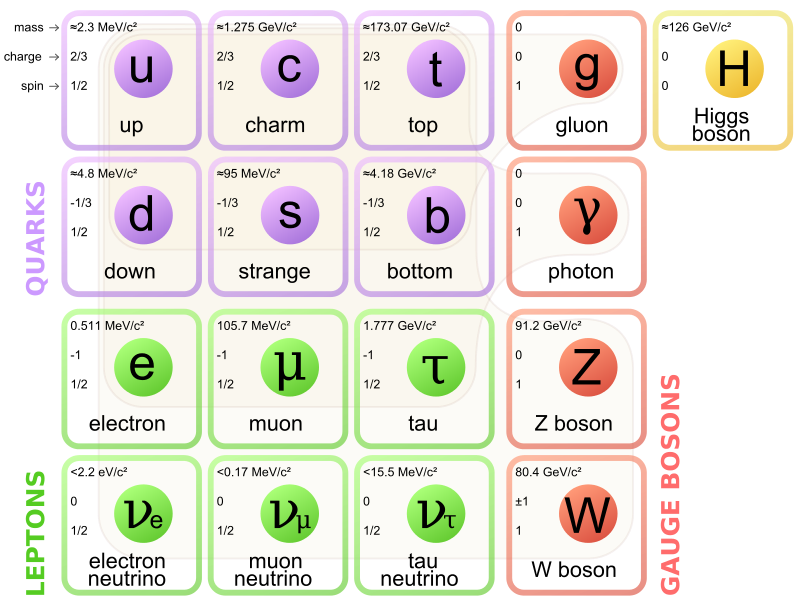
\includegraphics[scale=0.25]{img/particulelem}
		\captionof{figure}{Modèle standard des particules élémentaires}
	\end{center}
	Toutes les particules des trois premières colonnes sont des \textit{fermions} qui ont un spin de $1/2$ alors que la quatrième colonne est composée de \textit{vectoriel} qui ont un spin de 1 (le photon pouvant tourner dans les deux sens). La cinquième colonne n'a pas de spin, ce sont le(s) \textit{scalaire(s)}.\\
	Brièvement, ce sont les \textit{gluons} qui font tenir les particules positives ensemble dans le noyau.
	
	\section{Les quatre interactions fondamentales}
	Chacune sont attractive et/ou répulsive. La \textit{portée} est une longueur mesurant son rayon d'action. La force a une portée finie qui décroit d'un facteur $e$ sur chaque portée $a$ suivant :
	\begin{equation}
		V(r) \sim \frac{e^{-r/a}}{r}\ \ \ \ (r \mapsto \infty)
	\end{equation}
	\begin{center}
		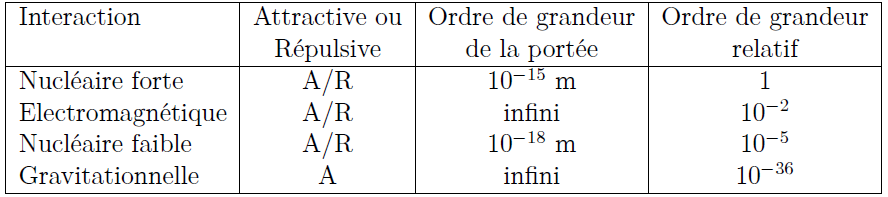
\includegraphics[scale=0.5]{img/interf}
		\captionof{figure}{Les 4 interactions}
	\end{center}
	Ces interactions fondamentales sont au nombre de quatre :
	\begin{enumerate}
		\item L'interaction gravitationnelle (échelle macroscopique)
		\begin{itemize}
			\item Toujours attractive mais très faible : aucun rôle en P.Q.
			\item Expliquée par une courbure de l'espace-temps par des \textit{géodésiques} : le plus court trajet entre deux points.
		\end{itemize}
		\item L'interaction électromagnétique (échelle macroscopique et microscopique)
		\begin{itemize}
			\item Attractive ou répulsive
			\item Explique la structure de la matière (cohésion des atomes et molécules): sera décrite dans le cours grâce aux potentiels (scalaire ou vecteur)
		\end{itemize}
		\item L'interaction nucléaire faible (aucun effet macroscopique car << inter. forte)
		\begin{itemize}
			\item Explique la désintégration $\beta$ à l'origine de l'instabilité du $n^0$ (souvent très lente car très faible et très courte portée\footnote{La portée est inversement proportionnelle à la masse de la particule échangée. Le boson de jauge ayant une grande masse, ça explique la courte portée. Pour l'EM, c'est infini car le photon à une masse nulle}).
			\item Relie hadrons et leptons
		\end{itemize}
		\item L'interaction nucléaire forte
		\begin{itemize}
			
			\item Assure la stabilité et la diversité de la matière (lie le noyau atomique (décrite par l'échange de \textit{gluons}))(cohésion des noyaux atomiques)
		\end{itemize}
	\end{enumerate}
	
	\subsection{Désintégration $\beta^-$ du neutron}
	\begin{center}
		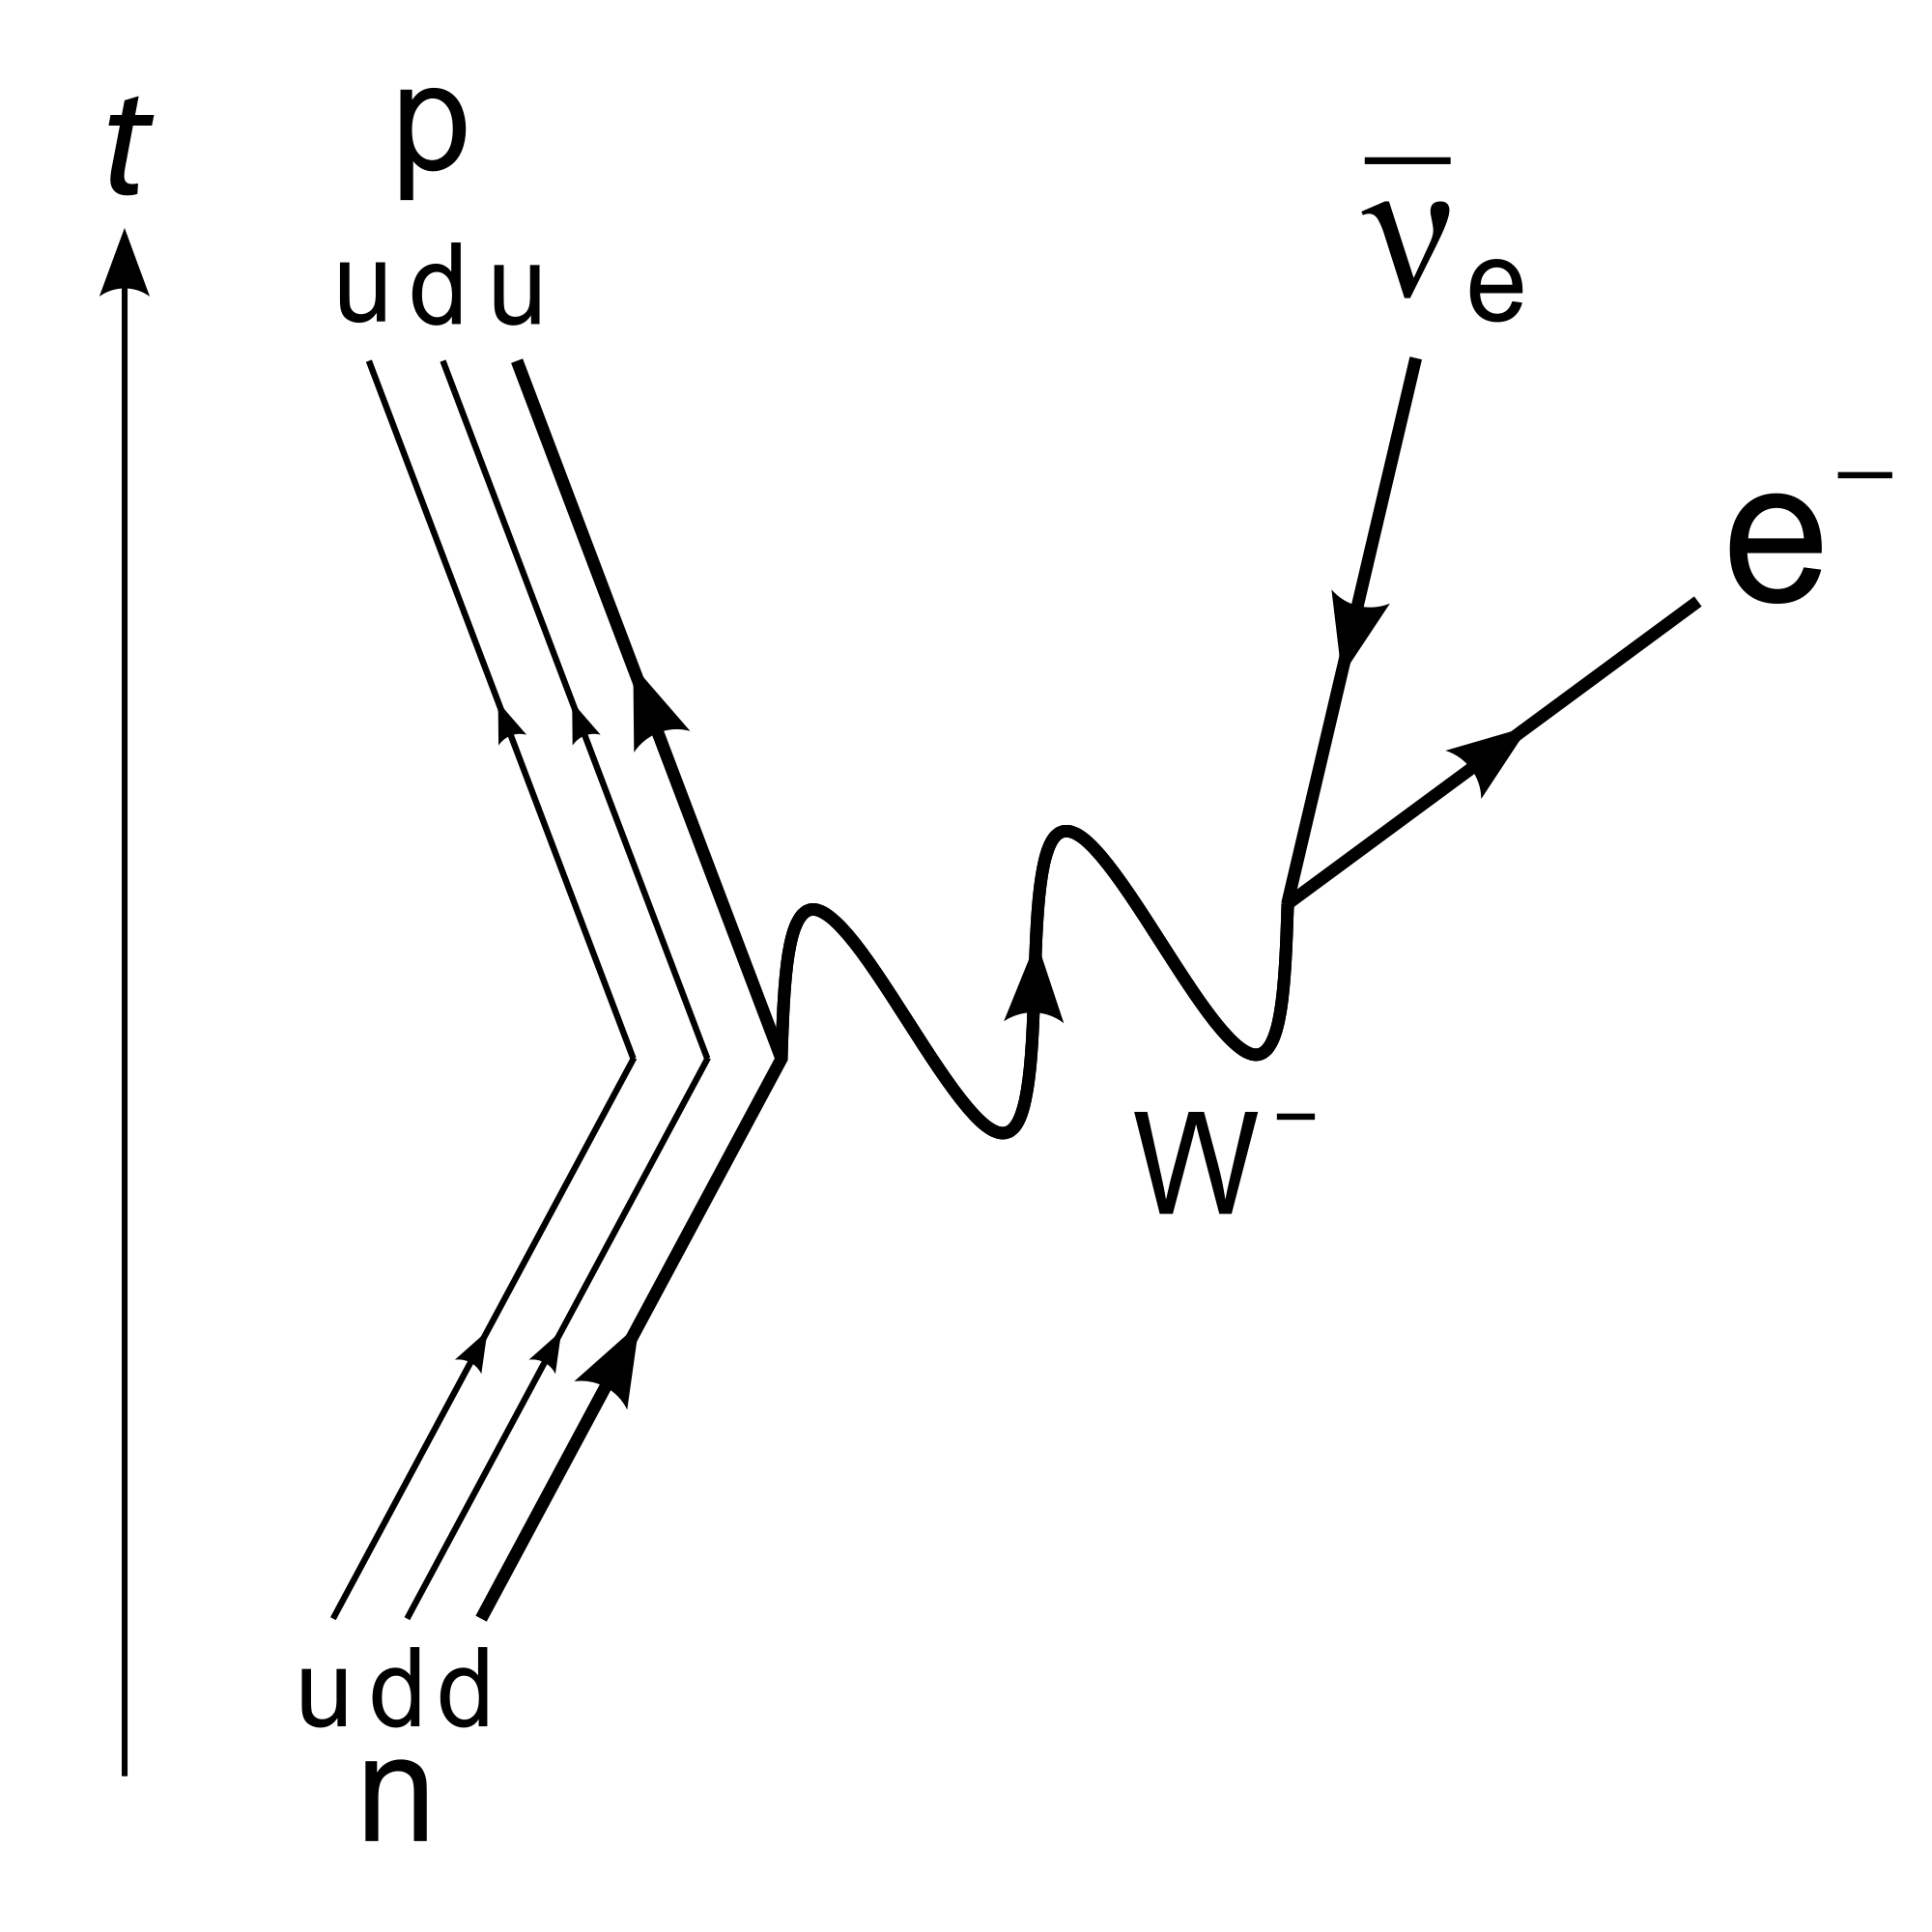
\includegraphics[scale=0.05]{img/beta}
		\captionof{figure}{Désintégration $\beta^-$ d'un neutron en termes de quarks}
	\end{center}
	C'est la désintégration $\beta$ qui rend le neutron (libre) instable, se désintégrant en un $p^+$, un $e^-$ et un $\bar v_e$ (anti-neutrino électronique) . Ceci s'explique par la transformation d'un quark down en un quark up au cours de l'émission d'un boson de jauge virtuel $W^-$, lui-même se désintégrant en un $e^-$ et un $\bar v_e$. De ces 2 leptons, seul l'$e^-$ est facilement détectable (d'où $\beta^-$, $\beta^+$ étant l'émission d'un $e^+$)\\
	
	La faiblesse de cette interaction rend la désintégration souvent très lente (ex : lenteur de l'évolution du soleil). La portée de l'interaction est proportionnelle à la masse de la particule échangée, la masse très élevée des bosons de jauge faibles rendent la portée de l'interaction très courte, alors que celle de l'interaction électromagnétique est infinie due à $m=0$ du photon.
	
	\section{Lois de conservations}
	On définit une \textit{loi de conservation} quand on suppose qu'une certaine grandeur est \textit{toujours} conservée lors d'interactions. Si un processus viole cette loi, il sera dit \textit{interdit}.\\
	Six lois sont importantes pour ce cours conservation de l'\textit{énergie}, de l'\textit{impulsion}, du \textit{moment cinétique}, de la \textit{charge}, du \textit{nombre leptonique} et du \textit{nombre baryonique}.
	
	
	\chapter{Les origines de la physique quantique}
	\setcounter{section}{-1}
	\section{Introduction (slides)}
	Alors que Newton pensait en 1704 que la lumière était des particules, Young proposa que la lumière était une onde. Selon son expérience, il y aura interférences constructives si :
	\begin{equation}
		d \sin \theta = n \lambda\ \ \ (n \in \mathbb{Z})
	\end{equation}
	
	\subsection{Les spectres atomiques}
	Kirchhoff envoyait de la lumière (type halogène) sur un gaz froid et mesurait la lumière transmise. En observant celle-ci, il a remarqué que certaines fréquences et $\lambda$ manquaient : \textit{raies d'absorption} qui correspondait précisément aux \textit{raies d'émission} : chaque élément a un spectre caractéristique.\\
	
	\textbf{Petit plus pour comprendre :} \textit{On sait que seuls certaines valeurs d'énergies sont accessible : les changements d'états correspondent donc eux aussi à des valeurs précises.}\ \\
	\textit{Un gaz chaud qui se refroidit émet des photons qui constitue un spectre composé d'un ensemble précis de raies lumineuse : les raies d'émission. Inversement,si le gaz froid est éclairé, il absorbera des photons et l'on parlera de raies d'absorption.}\ \\
	
	Balmer proposa plus tard une formule décrivant les longueurs d'ondes des raies et permettant la prédiction des raies invisibles :
	\begin{equation}
		\lambda_n = 364.6\frac{n^2}{n^2 - 4}\ nm
	\end{equation}
	Plus tard, Rydberg généralisa le résultat de Balmer en introduisant la \textit{constante de Rydberg} : $R = 0,01097\,nm^{-1}$ :
	\begin{equation}
		\frac{1}{\lambda_{n'n}} = R\left(\frac{1}{n'^2} - \frac{1}{n^2}\right)
	\end{equation}
	
	
	C'est ce qui était utilisé dans l'\textit{ancienne théorie des quanta} : pour un atome quelconque, on a donc :
	\begin{equation}
		\frac{1}{\lambda_{n'n}} = K_{n'} - K_n\quad\text{où}\ K_n=\frac{R}{n^2}
	\end{equation}
	Cela donnait comme interprétation des raies des sauts quantiques entre état d'énergie $E_n = hcK_n$.
	
	\section{La constante de Planck}
	C'est en essayant de décrire le corps noir\footnote{Rayonnement EM dans un four, voir partie \textit{Physique statistique}} que Planck a su quantifier l'énergie :  quantum d'énergie est proportionnel à la fréquence $\nu = \frac{\omega}{2\pi}$ et à une certaine constante (action\footnote{Car unité "énergie . temps"}) :
	\begin{equation}
		h \approx 6,63 \times 10^{-34}\ Js
	\end{equation}
	Cette constante a été rendue importante par Einstein qui a montré que la quantification n'était pas propre au corps noir mais à tout rayonnement (par étude de l'effet photoélectrique, la masse restant constante dans 2 expériences indépendantes) !
	
	\section{Particules de lumière}
	En interprétant le résultat de Planck (énergie quantifiée dans un corps noir), Einstein a proposé que le rayonnement quelconque ne peut exister que sous forme de quanta discrets d'énergie, c'est à dire de multiple entier d'une quantité proportionnelle à la fréquence de se rayonnement. Comme $\lambda$ et $\nu$ sont relié par $\lambda = c/\nu$ les formes d'énergies accessibles sont donné par :
	\begin{equation}
		E = h\nu
	\end{equation}
	\begin{wrapfigure}[7]{l}{6cm}
		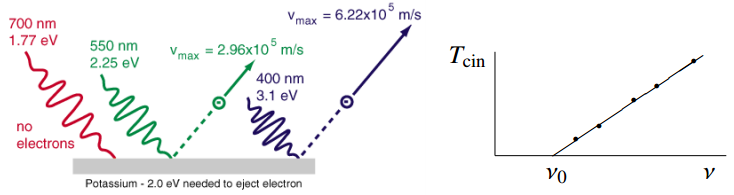
\includegraphics[scale=0.3]{img/image1.png}
		\captionof{figure}{Effet photoélectrique}
	\end{wrapfigure}
	Cette sainte formule explique l'effet photoélectrique. En envoyant de la lumière rouge sur un métal, rien ne se passe. Par contre en envoyant de la lumière verte (plus petite longueur d'onde $\rightarrow$ fréquence plus élevée $\rightarrow$ énergie plus grande) on arrive à extraire des électrons : il faut donc une fréquence "minimale" pour extraire un électron du métal\footnote{La pente de la droite vaut $h/e$ : la cste $h$ apparaît également ici !}.\\
	La lumière est constitué de quanta d'énergie et l'énergie d'un quantum est $\propto \nu$ : si l'énergie d'un quantum dépasse l'énergie de liaison des $e^-$ dans le métal un électron peut être arraché et le reste de l'énergie du quantum se retrouve sous forme d'énergie cinétique donné par :
	\begin{equation}
		T_{cin} = h\nu - W
	\end{equation}
	où $W$ est le travail pour extraire un électron. A $T_c = 0$, $W = h\nu_0$. Comme $\omega = 2\pi \nu = 2\pi c /\lambda$ on peut écrire :
	\begin{equation}\label{eq:ehbaromega}
		E = \hbar \omega
	\end{equation}
	Plus tard, Einstein proposa (1909) une relation liant le nombre d'onde et l'impulsion :
	\begin{equation}\label{eq:phbark}
		\vec{p} = \hbar \vec{k}
	\end{equation}
	En associant le nombre d'onde à l'impulsion, on peut écrire le \textit{quadrivecteur d'onde} :
	\begin{equation}\label{eq:Komegack}
		K = (\omega / c, \vec{k})
	\end{equation}
	Comme $E = h\nu$, $\nu = c/\lambda$ et $k = 2\pi/\lambda$ on sait que $\omega = kc$ on peut écrire que $E = pc$. Cette relation caractérise une particule de masse nulle : le \textit{photon}.\ \\
	La preuve expérimentale a été donnée par \textit{Comptons} en réalisant des collisions "photon-électron".\\
	
	\begin{center}
		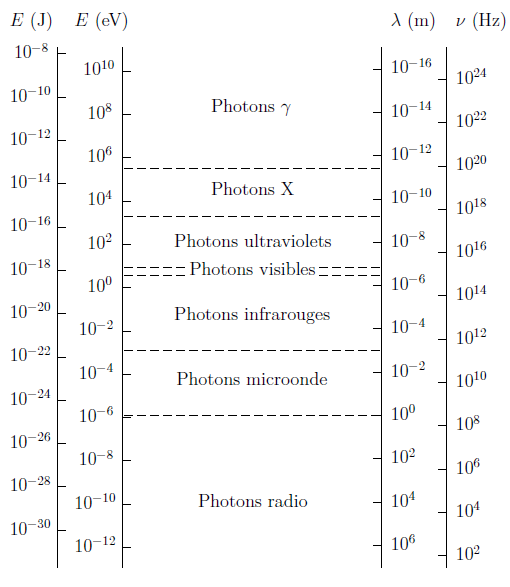
\includegraphics[scale = 0.5]{img/tableaucoeur}
		\captionof{figure}{Particule de rayonnement électromagnétique (\textbf{a connaître par coeur}}
	\end{center}
	\textit{Remarque :} \eqref{eq:ehbaromega} et \eqref{eq:phbark} unifié grâce à \eqref{eq:Komegack}$\Rightarrow P=\hbar K$\\
	\textit{NB :} $1\,eV=1,602\times 10^{-19}\,J$
	\section{Ondes de matière}
	En 1923, \textit{de Broglie} a avancé l'hypothèse qu'une onde est associée au mouvement de \textbf{tous} les types de particules (même celles sans masse) : \textit{ondes de matière}. La \textit{longueur d'onde de de Broglie} est donné par $\lambda = h/p$ : elle caractérise une onde qui accompagne le mouvement de la particule et dépend de sa vitesse. Si l'onde et la particule ont la même direction, on peut introduire un vecteur $\vec{k}$ pour ré-écrire la relation sous sa forme générale :
	\begin{equation}
		\vec p = \hbar \vec{k}
	\end{equation}
	La formule introduite pour le photon est donc valable \textbf{pour toute particule}.\\
	En se basant sur la notion relativiste du quadrivecteur, la relation précédente entraîne pour toute particule la relation :
	\begin{equation}
		E = \hbar\omega
	\end{equation}
	Lors de la propagation d'une onde, le lien entre $\omega$ et $\vec{k}$ est la \textit{relation de dispersion} : $\omega = f(k)$.\\
	
	\begin{wrapfigure}[9]{l}{4.5cm}
		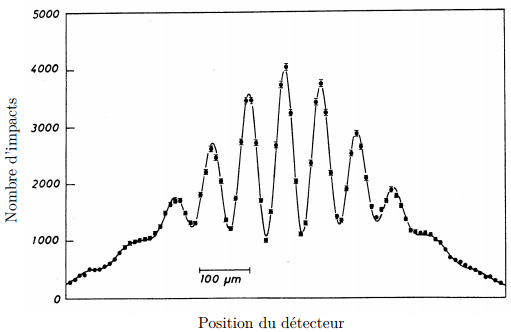
\includegraphics[scale=0.3]{img/image3.png}
		\captionof{figure}{Caractère ondulatoire de la matière}
	\end{wrapfigure}
	Pour mettre en évidence ce caractère ondulatoire de la matière, on a mené une série d'expérience ou l'onde associée au mouvement d'une particule/molécule est amenée à interférer avec elle-même (deux trous suffisamment proche pour ne pas négliger la longueur d'onde de de Broglie) donnant des figures d'interférences. En envoyant des particules à travers les fentes, on obtient des courbes représentant des maxima et des minima typiques de l’interférence de deux ondes.\\
	
	Cette expérience à ensuite été reproduite avec des systèmes plus complexe ($Na + Na_2$) envoyé simultanément entre deux fentes, à même vitesse. On observe sur la figure $(a)$ ci-dessous une superposition des franges qui seraient obtenues avec chacun des deux faisceaux séparé\footnote{La différence entre $(a)$ et $(b)$ donne les franges obtenues avec les atomes seuls}.
	\begin{center}
		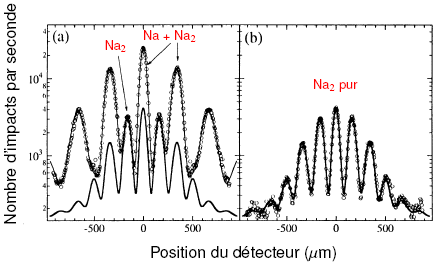
\includegraphics[scale=0.6]{img/image2.png}
		\captionof{figure}{Figure d'interférence}
	\end{center}
	Les franges obtenues avec les atomes seuls ont un espacement double des franges obtenues avec les molécules, ce qui est en accord avec $\lambda = h/p$ :
	\begin{equation}
		\frac{\lambda(Na)}{\lambda(Na_2)} = \frac{h/p(Na)}{h/p(Na_2)} = \frac{p(Na_2)}{p(Na)} = \frac{m(Na_2)}{m(Na)} = 2
	\end{equation}
	
	Les page 27 - 29 sont à lire à titre informatif.
	
	
	\chapter{L'équation de Schrödinger}
	\setcounter{section}{-1}
	\section{Équations d'ondes libres pour la lumière (Slide only)}
	\subsection{Électromagnétisme : formulation relativiste}
	Pour unifier l'électricité et le magnétisme en relativité restreinte, on défini le \textit{quadrivecteur potentiel} :
	\begin{equation}
		A \equiv \left(\frac{V}{c}, \vec A\right)
	\end{equation}
	où $V$ est le potentiel scalaire et $\vec A$ le potentiel vecteur, l'équivalent du potentiel scalaire pour le champ magnétique $\vec B$.\\
	On peut dès lors ($C.f.$ cours d'électricité) dire que $\vec{E} = -\vec{\nabla}V - \dfrac{\partial \vec A}{\partial t}$ et $\vec B = \vec{\nabla}\times \vec{A}=\text{rot }\vec A$. On y remarque que lorsque $\vec A$ varie dans le temps $\vec B$ est non nul. La division par $c$ permet d'obtenir la cohérence dimensionnelle ($m^{-1}$).\\
	
	De façon générale, on défini le \textit{quadrigradient} $\nabla$ et le \textit{quadrilaplacien} (ou \textit{d'Alembertien}, traduisant la courbure) $\square$ :
	\begin{eqnarray}
		\nabla &\equiv & \left(\frac{\partial}{c\partial t}, \vec{\nabla}\right)\\
		\square &\equiv &\nabla^2
	\end{eqnarray}
	En développant le d'Alembertien, on trouve : 
	\begin{equation}
		\square = \left(\frac{\partial}{c\partial t}, \vec{\nabla}\right) \circ \left(\frac{\partial}{c\partial t}, \vec{\nabla}\right) = \frac{\partial^2}{c^2\partial t^2} - \Delta = \epsilon_0\mu_0\frac{\partial^2}{\partial t^2} - \frac{\partial^2}{\partial x^2} - \frac{\partial^2}{\partial y^2} - \frac{\partial^2}{\partial z^2}
	\end{equation}
	L'équation d'onde est donc : $\square \vec B = 0$. Celles-ci sont :
	\begin{itemize}
		\item \textit{Invariantes relativistes} $\Rightarrow$ invariance de $c$ dans le vide (du au fait que la norme pseudo-euclidienne est valable partout : quelque soit le référentiel, on a la même équation d'onde ce qui implique l'invariance de $c$).
		\item Vectorielles et réelles
		\item Linéaires : combili = solution
		\item Aux dérivées partielles : résolution par \textit{transformée de Fourier} (phaseurs) $\vec{k}$ = nombre d'onde et $\omega$ est la fréquence angulaire
		\item Interprétation : comme le photon à une masse nulle et qu'il se déplace à vitesse $c$, il ne peut accélérer
	\end{itemize}
	\begin{equation}
		\vec{B}_{\vec{k}}(\vec{r},t) = \text{Re}\ \left[\underline{\vec{B}_0}e^{i(\vec{k}\vec{r}-\omega t)}\right]
	\end{equation}
	\subsection{Électromagnétisme : ondes planes et paquets d'ondes}
	La transformée de Fourier permet de passer d'une équation aux dérivées partielles en équation algébrique (relation de dispersion).
	\begin{equation}
		\frac{\partial}{\partial t} \rightarrow \times(i\omega),\ \ \ \ \ \vec{\nabla} \rightarrow \times (i\vec{k})
	\end{equation}
	En appliquant ce principe, on trouve pour $\square \vec{B} = 0$ :
	\begin{equation}
		-\frac{\omega^2}{c^2} + k^2 = 0 \Leftrightarrow \omega(k) = kc \Leftrightarrow \nu : \frac{c}{\lambda}
	\end{equation}
	
	\section{Origine}
	A chaque particule est associée une onde, c'est ce qui a été découvert par \textit{de Broglie}. Une fois ces ondes découvertes, on a commencé à chercher leur équation et c'est à \textit{Erwin Schrödinger} que revient le mérite. Son équation permet d'expliquer \textit{tous} les résultats expérimentaux connus à ce jours dans la mesure ou des calculs suffisamment précis sont possibles.
	\section{Équation d'onde d'une particule libre}
	Une particule est libre quand elle n'est soumise à aucune interaction extérieure et son mouvement peut être entièrement caractérisé par sa masse $m$ et 2 grandeurs indépendantes : $\vec p$ et $E$.\footnote{Les autres n'interviennent pas ici.}\\
	Le mouvement d'une particule est rectiligne, il est naturel de lui associer une onde qui se propage de la sorte :
	\begin{equation}
		\psi (\vec{r}, t) = e^{i(\vec{k}.\vec{r} - \omega t)}
	\end{equation}
	On sait que le \textit{nombre d'onde} $k$ est relié à $\lambda$ et que $\omega$ est relié à la fréquence $\nu$. L'onde se propage à la \textit{vitesse de phase} $\omega/k$. Les grandeurs $\vec{k}$ et $\omega$ sont reliées par une \textit{relation de dispersion}.\\
	
	Quand $E(p)$ ne représente que l'énergie purement cinétique dans un contexte non-relativiste, celle-ci vaut :
	\begin{equation}
		E(p) = p^2/2m=T
	\end{equation}
	En utilisant $\vec{p} = \hbar \vec{k}$ et $E = \hbar\omega$ on trouve la relation de dispersion d'une onde accompagnant une particule massive non relativiste
	\begin{equation}
		\omega (k) = \hbar k^2/2m
	\end{equation}
	Dans un espace à une dimension, on aurait alors : 
	\begin{equation}
		\psi_k(x,t) = e^{i[kx -(\hbar k^2/2m)t]}
	\end{equation}
	Cherchons une ED dont toutes ces ondes planes sont solutions. La dérivée par rapport à $t$ donne un terme $\propto k^2$ alors que la dérivée seconde par rapport à $x$ est $\propto k$\footnote{Voir le principe de correspondance dans les slides}.
	\begin{equation}
		\frac{\partial}{\partial t} \Rightarrow k^2,\ \ \ \ \frac{\partial}{\partial x} \Rightarrow k,\ \ \ \ \frac{\partial^2}{\partial x^2} \Rightarrow k^2
	\end{equation}
	Comme $\frac{\partial^2 \psi}{\partial x^2}=-k^2$ et $\frac{\partial\psi}{\partial t}=-i\hbar\frac{k^2}{2m}$, on trouve dès lors l'équation recherchée :
	\begin{equation}
		i\hbar \frac{\partial \phi_k}{\partial t} = -\frac{\hbar^2}{2m}\frac{\partial^2 \phi_k}{\partial x^2}
	\end{equation}
	Comme cela ne dépend pas de $k$, Erwin a postulé que la \textit{fonction d'onde} $\psi (x,t)$ est une solution de l'équation aux dérivées partielles : 
	\begin{equation}
		i\hbar \frac{\partial \psi}{\partial t} = -\frac{\hbar^2}{2m}\frac{\partial^2 \psi}{\partial x^2}
	\end{equation}
	Il s'agit d'une équation \textit{linéaire} et \textit{complexe} tandis que $\phi$ est la \textit{fonction d'onde}.\\
	
	
	Cette équation possède des \textit{solutions particulières séparables} qui a dès lors pour solution générale :
	\begin{equation}
		\psi (x,t) = \int_{-\infty}^{+\infty} C(k).e^{i(\vec{k}.\vec{r} - \omega t)}
	\end{equation}
	où $C$ est une fonction complexe arbitraire de $k$.\\
	Cette combinaison linéaire est souvent appelées \textit{paquet d'onde}.\\
	
	Supposons que $C(k)$ ne prenne des valeurs non négligeable que sur un intervalle $\Delta k$ autour d'une valeur $k_0\neq0$\\
	La contribution principale de l'intégrale provient des valeurs $\in\Delta k$, en partant de la relation de dispersion \begin{align}
		\omega(k) & =\frac{\hbar k^2}{2m}=\frac{\hbar}{2m}\underbrace{[k_0^2+2k_0(k-k_0)+(k-k_0)^2]}_{k^2}\\
		& =\omega_0+v(k-k_0)+\frac{\hbar}{2m}(k-k_0)^2 &\text{avec } \omega_0=\omega(k_0),\qquad v_g=\dfrac{\hbar k_0}{m}
	\end{align}
	
	Si on néglige le dernier terme, on obtient \begin{equation}\psi(x,t) \approx e^{-i(\omega_0-vk_0)t}\int^{+\infty}_{-\infty}C(k)e^{ik(x-vt)}dk
	\end{equation}
	La fonction réelle $|\psi|^2$ se propage a vitesse $v$ sans se déformer (du moins tant que l'approximation reste reste valable). \\
	Cette équation nous montre que le paquet d'ondes se propage comme une particule libre à condition d'interpréter la vitesse de groupe comme la vitesse de déplacement de la particule. L'onde et la particule se propage ensemble (mais aucune autre information!).\\\\
	L'approximation est valable si (temps court)
	\begin{equation}\frac{\hbar\Delta k^2t}{2m}\ll1\Leftrightarrow t\ll\frac{2m}{\hbar\Delta k^2}\end{equation}
	Si plus satisfaite $\Rightarrow$ l'approximation fausse $\Rightarrow$ \textit{Étalement du paquet d'ondes} dû à la relation de dispersion, les ondes qui constituent le paquet n'ont pas la même vitesse de phase (car dépend de $k$) et donc finissent par se disperser. Plus $\Delta k$ est petit, plus l'étalement se fait lentement.
	\paragraph{Rappel :}
	\begin{equation}
		\begin{array}{cc}
			v_g=\frac{d\omega}{dk} & v_{\varphi}=\frac{\omega}{k} 
		\end{array}{}
	\end{equation}
	\section{Particule dans un puits de potentiel}
	Comme en mécanique classique, on peut écrire que l'énergie est la somme d'une énergie potentiel et cinétique, ce qui sera repris dans une fonction $H$, l'Hamiltonien (représente l'énergie totale), fonction de la position et de l'impulsion :
	\begin{equation}
		E = T + V(\vec{r}) = \frac{\vec{p}^2}{2m} + V(\vec{r}) \equiv H
	\end{equation}
	En appliquant la règle de correspondances :
	\begin{equation}
		E \rightarrow i\hbar \frac{\partial}{\partial t},\qquad p_x \rightarrow i\hbar\frac{\partial}{\partial x},\qquad 3D: \vec p=-i\hbar\vec{\nabla}
	\end{equation}
	On obtient une équation aux dérivées partielles linéaire et homogène\footnote{Formule à connaître \textbf{par cœur}} (en généralisant en 3D)
	\begin{equation}
		i\hbar \frac{\partial \psi}{\partial t} = -\frac{\hbar^2}{2m}\Delta\psi+ V(\vec r)\psi
	\end{equation}
	On peut faire apparaître le fameux opérateur $H$ défini un peu plus haut pour avoir :
	\begin{equation}
		i\hbar \frac{\partial \psi}{\partial t} = \left[-\frac{\hbar^2}{2m}\Delta + V(\vec{r})\right]\psi(\vec{r},t) \equiv H\psi(\vec{r},t)
	\end{equation}
	On y retrouve :
	\begin{itemize}
		\item L'énergie cinétique est un opérateur différentiel : $T = \frac{\vec{p}^2}{2m} = -\frac{\hbar^2}{2m}\Delta$
		\item L'énergie potentielle est un opérateur multiplicatif : 
		$V(\vec{r})$
		\item L'énergie total est un opérateur hamiltonien : $H = -\frac{\hbar^2}{2m}\Delta + V(\vec{r})$
		\item Une zone interdite : $V(\vec{r}) = \infty$ impose par condition au limites que $\psi(\vec{r}, t) = 0\ \forall t \rightarrow$ diffraction et séparation du paquet d'onde (voir exemples slides 10)
	\end{itemize}
	
	\section{Équation de Schrödinger stationnaire}
	\subsubsection*{Potentiel $V$ indépendant du temps}
	Dans ce cas-ci, on peut chercher des solutions de l'équation $i\hbar\frac{\partial\psi}{\partial t}=\left[\frac{p^2}{2m}+V(\vec r)\right]\psi $ par la méthode de séparation des variables (Annexe 3C). Posons $\psi(\vec{r},t) = \chi(t)\phi(\vec{r})$\footnote{On sépare les variables d'espace et temporelle} et remplaçons-la dans l'équation d'onde que nous venons d'obtenir :
	\begin{equation}
		i\hbar \phi(\vec{r})\frac{d}{dt}\chi(t) = \chi(t)\left[-\frac{\hbar^2}{2m}\Delta + V(\vec{r})\right]\phi(\vec{r})
	\end{equation}
	En divisant tout par $\psi$:
	\begin{equation}\label{eq:3.21}
		i\hbar\frac{1}{\chi}\frac{d\chi}{dt} = \frac{1}{\phi(\vec{r})}\left[-\frac{\hbar^2}{2m}\Delta\phi(\vec{r}) + V(\vec{r)}\phi(\vec r)\right] \equiv E
	\end{equation}
	Le membre de gauche ne dépend que de $t$ et le second que de $\vec{r}$. Comme ils sont égaux $\forall t, \vec{r}$ ils doivent être constant : $E$. Ainsi, la \textit{constante de séparation} $E$ est l'énergie de la particule :
	\begin{equation}
		i\hbar \frac{d\chi}{dt} = E\chi
	\end{equation}
	Cette équa diff du premier ordre se résout facilement :
	\begin{equation}
		\chi(t) = \chi(0)e^{-iEt/\hbar}
	\end{equation}
	
	\subsubsection*{Dépendance spatiale}
	Égalons la partie en $\vec{r}$ de l'équation \eqref{eq:3.21} à $E$ - c'est l'\textit{équation de Schrödinger stationnaire}
	\begin{equation}
		-\frac{\hbar^2}{2m}\Delta\phi(\vec{r}) + V(\vec{r})\phi(\vec{r}) = E\phi(\vec{r})
	\end{equation}
	Grâce à l'opérateur hamiltonien, l'équation stationnaire peut aussi s'écrire, en multipliant par $\phi$ l'équation \eqref{eq:3.21} ) :
	\begin{equation}
		H\phi(\vec{r}) = E\phi(\vec{r})
	\end{equation}
	En choisissant $\chi(0) = 1$ la fonction d'onde $\psi(\vec{r},t) = \chi(t)\phi(\vec{r})$ devient : 
	\begin{equation}
		\psi(\vec{r},t) = e^{-iE_jt/\hbar}\phi_j(\vec{r})
	\end{equation}
	La solution générale n'est alors qu'une combinaisons linéaires de cette solution !\\
	
	Notons la condition aux limites : $\phi(\vec{r}) = 0$ si $V(\vec{r}) = \infty$. C'est par exemple les modes propres de vibration d'une corde/membrane.
	
	\chapter{Principes de la mécanique quantique}
	L'ordre des sections par rapport au syllabus est un peu modifiée, pour suivre (au mieux) le déroulement des slides.
	\setcounter{section}{2}
	\section{Postulat sur l'état d'un système}
	Commençons par le \textsc{Postulat I} (\textit{sur l'état d'un système (une particule)) :}
	\begin{center}
		L'état physique d'une particule à un instant $t$ est caractérisé par une \textbf{fonction d'onde complexe normée} $\psi(\vec{r},t)$. Le carré du module $|\psi(\vec{r},t)|^2$ de cette fonction donne la \textbf{densité de probabilité de présence} de cette particule au point $\vec{r}$ à l'instant $t$.
	\end{center}
	La particule n'est plus déterminée mais juste caractérisée par des probabilités de présence $\mathcal{P}(D,t)$ dans le domaine $D$ à l'instant $t$ :
	\begin{equation}
		\mathcal{P}(D,t) = \int_D |\psi(\vec{r},t)|^2 d\vec{r}
	\end{equation}
	Pour un instant $t$, on prépare $N$ systèmes identiques dans le même état (même $\psi$) et on détermine pour chacun si la particule est dans le domaine $D$. Le nombre de systèmes pour lesquels la particule est dans $D$ est noté $n(D,t)$. On trouve alors la probabilité de présence expérimentale :
	\begin{equation}
		\mathcal{P}_{exp}(D,t) = \lim\limits_{N \rightarrow \infty} \frac{n(D,t)}{N}=\frac{\text{nbre de cas favorables}}{\text{nbre de cas totaux}}
	\end{equation}
	La densité de probabilité étant $\rho(\vec{r}, t) = |\psi(\vec{r},t)|^2$ et en considérant un domaine $D$ représenté par $d\vec{r} = dxdydz$, appliquer le théorème de la moyenne à $\mathcal{P}(D,t)$ donne:
	\begin{equation}
		\mathcal{P}(d\vec{r},t) = \rho(\vec{r},t)d\vec{r}
	\end{equation}
	La densité $\rho(\vec{r},t)$ est la probabilité de présence par unité de volume. La seule certitude est de toujours retrouver la particule si on intègre l'espace accessible tout entier:
	\begin{equation}
		\mathcal{P}(\mathbb{R}^3,t) = \int_{\mathbb{R}^3} |\psi(\vec{r},t)|^2 d\vec{r}  \equiv||\psi(t)||^2 = 1
	\end{equation}
	La fonction d'onde doit donc être normée ce pourquoi on travaille sur l'ensemble des carrés sommables\footnote{Une fonction mesurable $f$ de $\mathbb{R}^3$ dans $\mathbb{C}$ est de carré sommable lorsque l'intégrale $\int_\mathbb{R} |f(x)|^2dx$ converge.}.
	
	\setcounter{section}{6}
	\section{Principe de superposition, chat de Schrödinger et ordinateurs quantiques}
	Soit deux fonctions d'ondes $\psi_1(\vec{r},t)$ et $\psi_2(\vec{r},t)$ avec $\rho_i(\vec{r},t) = |\psi(\vec{r},t)|^2$. \\
	\textit{Toute combinaison linéaire normée de fonctions d'onde est une fonction d'onde.}
	\begin{equation}
		\psi(\vec{r},t) = \lambda_1\psi_1(\vec{r},t) + \lambda_2\psi_2(\vec{r},t), \ \ \ \ \ \lambda_1,\lambda_2 \in \mathbb{C}
	\end{equation}
	
	La densité de probabilité de ces deux ondes fait apparaître un terme d'interférence
	\begin{equation}
		\rho(\vec{r},t) = \psi^*(\vec{r},t)\psi(\vec{r},t) = |\lambda_1|^2\rho_1(\vec{r},t) + |\lambda_2|^2\rho_2(\vec{r},t) + 2\text{Re}\underbrace{\lambda_1^*\lambda_2\psi_1^*(\vec{r},t)\psi_2(\vec{r},t)]}_{\text{Interférence}}
	\end{equation}
	On voit apparaître le problème du principe de superposition. L'état étant à moitié $\psi_1$ et à moitié $\psi_2$, la densité correspondante n'est pas la demi-somme des deux densité de probabilités, il y a un terme additif qui représente l'interférence entre les deux composantes : les états sont dit \textit{enchevêtrés}.\\
	Cela conduit à l'interprétation de la fonction d'onde :
	\begin{itemize}
		\item Mathématiquement ("interprétation de Copenhague"à la fonction d'onde est une amplitude de probabilité\footnote{Fonction à valeurs complexes associée à la probabilité de trouver le système dans un état particulier.}
		\item Physiquement : la fonction d'onde est une onde porteuse
	\end{itemize}
	
	\setcounter{section}{4}
	\section{Postulat d'évolution	}
	\textsc{Postulat VI} (Évolution du système) :
	\begin{center}
		L'évolution du système au cours du temps est régie par l'équation de Schrödinger
		\begin{equation}
			i\hbar \frac{\partial \psi(t)}{\partial t} = H\psi(t)
		\end{equation}
		où $H$ est l'observable (opérateur) associée à l'énergie du système
	\end{center}
	On postulera que l'opérateur $H$ existe toujours : sa "bonne" forme se fait par comparaison des résultats de l'équation de Schrödinger avec l'expérience.\\
	
	Il s'agit d'une ED d'ordre 1 vis-à-vis du temps. Il suffit de choisir une fonction d'onde initiale à un instant donné pour déduire la fonction d'onde : l'évolution est déterministe et dicté par les C.I.\\
	Mais, l'information que l'on pourra obtenir sur le système sera probabiliste et ce à tout instant.\\
	Notons également que l'opérateur hamiltonien $H$ étant linéaire, il obéit au principe de superposition.
	
	\setcounter{section}{0}
	\section{Propriétés mathématiques}
	On travaille dans l'espace des \textit{fonctions de carré sommable} $L^2(\mathbb{R}^3)$ en considérant le sous-ensemble des fonctions dérivables deux fois $L^2(\mathbb{R}^3)\cap C^2(\mathbb{R}^3)$.\\
	Dans cet espace\footnote{Notons qu'il s'agit d'un espace fonctionnel de dimension infinie. Les ondes planes ne font pas partie de cet ensemble mais les paquets d'onde bien.}, le \textit{produit scalaire} (de deux fonctions) est défini par
	\begin{equation}
		\left\langle\phi|\psi\right\rangle = \underbrace{\int d\vec{r}\, \phi^*(\vec{r})}_{\text{"bra"}}\underbrace{\psi(\vec{r})}_{\text{"ket"}}
	\end{equation}
	On peut retrouver (Cf. \textit{Mécanique Quantique I}) ce produit grâce à la notation de Dirac :
	\begin{itemize}
		\item "ket" $|\psi\rangle$ = élément de l'espace fonctionnel
		\item "bra" $\langle\phi|$ = élément de l'espace dual (forme $L^2 \rightarrow \mathbb{C} : |\psi\rangle \rightarrow \langle \phi|\psi\rangle$)
	\end{itemize}
	Les fonctions d'ondes physiques sont donc de carrés sommables et possède une norme définie par
	\begin{equation}
		||\psi|| = \langle \psi|\psi\rangle^{1/2} = \left[\int |\psi(\vec{r}|^2d\vec{r}\right]^{1/2} < \infty
	\end{equation}
	
	\subsection*{Opérateurs et opérateurs hermétiques (Cf. Algèbre linéaire)}
	Un opérateur $A$ transforme une fonction en une autre
	\begin{equation}
		\phi(\vec{r}) = A\psi(\vec{r})
	\end{equation}
	
	Une \textit{fonction propre} $u_a(\vec{r})$ de l'opérateur $A$ est une fonction non nulle telle que $Au_a(\vec{r}) \propto u_a(\vec{r}) \forall \vec{r}$ :
	\begin{equation}
		Au_a(\vec{r}) = au_a(\vec{r})
	\end{equation}
	où $a$ est la valeur propre correspondante. Lorsque tous les fonctions propres $u_a$ associé à une valeur propre $a$ sont $\propto$ cette valeur propre est \textit{non dégénérée} (\textit{dégénérée} dans le cas contraire).\\
	L'EV de fonctions linéairement indépendante associé à une même valeur propre (au moins 2) est le \textit{sous-espace propre} de cette valeur propre est est de même dimension que le \textit{degré de dégénérescence} $d_a$ de cette valeur propre.\\
	
	L'ensemble des valeurs propres de $A$ constitue le \textit{spectre} de cet opérateur. Il peut être discret (isolé) ou continu (non isolé).
	
	Un opérateur $A$ est  hermétique\footnote{Notons pour la suite que toutes les valeurs propres d'un opérateur hermétique sont réelles.} ssi
	\begin{equation}
		\int \phi^*(\vec{r})A\psi(\vec{r})d\vec{r} = \left[ \int\psi^*(\vec{r})A\phi(\vec{r})d\vec{r} \right]^*, \ \ \ \forall \phi, \psi
	\end{equation}
	Ce qui peut s'écrire plus simplement grâce aux règles de Diract : $\langle \phi|A|\phi \rangle = \langle\psi|A|\phi\rangle^*$.\\
	Dans le cas particulier ou $\psi =  \phi$ on trouve : $\langle\psi|A|\psi\rangle = \langle\psi|A|\psi\rangle^*$.
	
	\subsection*{Observables et commutateurs}
	Un \textit{observable} est un opérateur hermétique dont les fonctions propres forment un \textit{ensemble complet}\footnote{Toute fonction de $L^2(\mathbb{R}^3)$ possède un développement de Fourier sur la base constituée par ses fonctions propres (c'est à dire que $\{u_a(\vec{r})\}$ = base).}\\
	Nous admettrons que les principaux opérateurs hermétiques possédant un sens physique sont des observables (dans ce cours).\\
	
	Le produit d'opérateur est en général non commutatif : $AB\psi(\vec{r}) \neq BA\psi(\vec{r})$. On défini ainsi l'opérateur \textit{commutateur} de A et B :
	\begin{equation}
		[A, B] = AB - BA
	\end{equation}
	On en tire le théorème :\\
	\textit{Deux observables $A$ et $B$ commutent $\Leftrightarrow$ elles possèdent un ensemble complet (base) de fonction propres communes $u_{ab}$}.\\
	\begin{proof}\ \\
		\begin{eqnarray}
			\left\{\begin{array}{l}
				Au_{ab}=au_{ab}\\
				\\
				Bu_{ab}=bu_{ab}
			\end{array}\right.\Rightarrow[A,B]u_{ab} &=& (AB-BA)u_{ab}=(ABu_{ab}-BAu_{ab})\\
			&=& (Abu_{ab}-Bau_{ab})=(Au_{ab}b-Bu_{ab}a)\\
			&=& (ab-ba)u_{ab}=0\\
			\Rightarrow AB-BA=0\Rightarrow AB=BA
		\end{eqnarray}
	\end{proof}
	
	\setcounter{section}{3}
	\section{Postulats sur les mesures}
	\textsc{Postulat II} (Description des grandeurs physiques) :\\
	\textit{Une grandeur physique mesurable est décrite par une observable.}\\
	Une grandeur physique est mesurable avec un appareil et un observable est un objet mathématique (opérateur hermétique avec base d'états propres).\\
	
	La construction des observables se fait par la règle de correspondance :
	\begin{equation}
		A(\vec{r},\vec{p}) \rightarrow \text{opérateur }A(\vec{r}, -i\hbar\vec{\nabla})
	\end{equation}
	Il faut avant tout \textbf{symétriser} les opérateurs qui ne commutent pas. Par exemple\footnote{On ne peut pas remplacer $\vec{p}$ par $i\hbar\vec{\nabla}$ sans écrire l'expression sous "forme correcte" (Cf. 4.6).}, $\vec{r}.\vec{p} \rightarrow \frac{1}{2}(\vec{r}.\vec{p}+\vec{p}.\vec{r}) = -\frac{1}{2}i\hbar(\vec{r}.\vec{\nabla} + \vec{\nabla}.\vec{r})$.\\
	
	\textsc{Postulat III} (Mesure d'une grandeur physique):\\
	\textit{La mesure d'une grandeur physique ne peut donner comme résultat qu'une des \textbf{valeurs propres $a$} de l'\textbf{observable $A$} correspondante.}\\
	
	Ainsi, si l'observable à des valeurs propres discrètes, seules ces valeurs la pourront être obtenues : \textit{quantification} des résultats. Par exemple pour Schrödinger stationnaire $H\phi(\vec{r}) = E\phi(\vec{r})$ l'énergie sera quantifiée : $E_i$.\\
	
	\textsc{Postulat IV} (Probabilité d'un résultat) :\\
	\textit{On mesure une grandeur physique décrite par l'observable $A$ sur un système dont la fonction d'onde est $\psi(\vec{r},t)$. La probabilité d'obtenir comme résultat de la mesure la valeur propre $a$ de l'observable est donnée par\footnote{Valeurs propres discrètes et non dégénérée.}}:
	\begin{equation}
		\mathcal{P}(a,t) = |\langle u_a|\psi\rangle|^2
	\end{equation}
	\textit{où $u_a$ est la fonction propre normée de $A$ correspondant à la valeur propre $a$.}\\
	On retrouve bien la certitude d'avoir un résultat : $\sum_a \mathcal{P}(a,t) = 1$.
	
	\subsection*{Valeur moyenne et écart quadratique moyen (Slides)}
	Soit un grand nombre de particules de fonction d'onde $\psi(\vec{r})$. Pour chaque position on a une probabilité de présence de la particule. On peut en calculer la valeur moyenne\footnote{Ne pas confondre moyenne et Dirac!} 
	\begin{equation}
		\langle x \rangle_\psi = \int x\rho(\vec{r})d\vec{r} = \int \psi^*(\vec{r})x\psi(\vec{r})d\vec{r} = \langle \psi|x|\psi\rangle
	\end{equation}
	Ce résultat peut être généralisé à une observable $A$ quelconque
	\begin{equation}
		\sum_a a\mathcal{P}(a)
	\end{equation}
	L'écart quadratique moyen ou \textit{incertitude} sur $x$ :
	\begin{equation}
		(\Delta x)_\psi = \left[\int(x-\langle x\rangle_\psi\rho(\vec{r})d\vec{r}\right]^{1/2} = \left\langle\left(x-\langle x\rangle_\psi\right)^2\right\rangle^{1/2}_\psi
	\end{equation}
	Ce résultat se généralise également (remplacer $x$ par $A$).
	
	
	
	\setcounter{section}{7}
	\section{Relations d'incertitudes de Heisenberg}
	Heisenberg met en évidence le caractère probabiliste de la physique quantique. Commençons d'abord par introduire la \textit{valeur moyenne}
	\begin{equation}
		\langle x \rangle_\psi = \int x\rho(\vec{r})d\vec{r} = \int x|\psi(\vec{r})|^2d\vec{r} = \int \psi^*(\vec{r}) x \psi(\vec{r}) d\vec{r}
	\end{equation}
	On peut avoir une définition plus générale en remplaçant $x$ par une observable $A$ (comme l'impulsion $p_x$ par exemple)
	\begin{equation}
		\langle A \rangle_\psi = \int \psi^*(\vec{r}) A \psi(\vec{r}) d\vec{r}
	\end{equation}
	Comme pour toute variable aléatoire, on peut compléter la notion de valeur moyenne par celle d'écart quadratique moyen :
	\begin{equation}
		(\Delta A)_\psi = \langle(A-\langle A \rangle_\psi)^2\rangle^{1/2}_\psi 
	\end{equation}
	Ce qui est "l'incertitude". \\
	
	Considérons deux observables $x$ et $p_x$, une relation les liant est\footnote{Annexe 4C} :
	\begin{equation}
		(\Delta x)_\psi (\Delta p_x)_\psi \geq \frac{1}{2}\hbar
	\end{equation}
	Il s'agit de la \textit{relation d'incertitude entre la position et l'impulsion.} Chacune des incertitudes $(\Delta x)_\psi$ ou $(\Delta p_x)_\psi$ peut être rendue très petite (mais $\neq 0$) mais l'autre devra alors être très grande.\\
	Des observables qui vérifient 
	\begin{equation}
		[A,B] = i\hbar
	\end{equation}
	sont dites \textit{conjuguées canoniquement}. Pour ce genre d'observable, on obtient la relation précédente, généralisée :
	\begin{equation}
		(\Delta A)_\psi (\Delta B)_\psi \geq \frac{1}{2}\hbar
	\end{equation}
	Ceci n'a rien à voir avec une imprécision mais juste l'impossibilité de réaliser un état physique pour lequel les incertitudes sont simultanément très petites.
	
	\setcounter{section}{6}
	\section{Principe de superposition, chat de Schrödinger et ordinateurs quantiques (suite)}
	Un appareil de mesure est un système physique dont la fonction d'onde $M$ doit être couplée à la fonction d'onde $\psi$ du système microscopique mesuré : $\psi_1 \rightarrow M_1, \psi_2 \rightarrow M_2$.\\
	Le système macro doit décrire des termes quantiques ce qui n'est pas toujours possible. Le principe de superposition n'a pas d'équivalent apparent à l'échelle macroscopique. On est face au problème de la superposition d'états macroscopiques distincts.
	\begin{equation}
		\lambda_1\psi_1 + \lambda_2\psi_2 \rightarrow \lambda_1M_1 + \lambda_2M_2
	\end{equation}
	Cela signifie que le grain est à la fois à la position 1 et à la position 2, ce qui n'est pas possible à l'échelle macroscopique.\\
	Le paradoxe du chat de Schrödinger souligne cela.
	
	\subsection*{Décohérence}
	Un système macroscopique n'est jamais dans une superposition d'état\footnote{Une aiguille ne peut être sur 1 et 7 en même temps.}. Ceci est du à la décohérence, c'est à dire la perte de cohérence entre les états superposés due à l'environnement\footnote{Ce qui l'entoure, } et surtout irréversible. C'est le fait que la fonction d'onde cesse d'être valable.
	\begin{equation}
		\lambda_1M_1 + \lambda_2M_2 \rightarrow M_1\ \textit{où}\ M_2
	\end{equation}
	On part d'une superposition linéaire vers la décohérence ou  l'on a soit $M_1$, soit $M_2$.\\
	La décohérence pour le compter Geiger se produit tellement vite que tout effet quantique devient inobservable sur le chat.\\
	Ne pervenant pas à modéliser ceci, on défini le postulat de réduction de la fonction d'onde :\\
	
	\textsc{Postulat V} (Réduction de la fonction d'onde) :\\
	\textit{Immédiatement après une mesure sur la grandeur physique décrite par l'observable $A$ qui a donné le résultat $a$, la fonction d'onde du système est égale à la fonction propre normée $u_a(\vec{r})$ de $A$ correspondant à la valeur propre $a$,}
	\begin{equation}
		\tilde{\psi}(\vec{r},t) = u_a(\vec{r})
	\end{equation}
	Si on recommence la mesure immédiatement après, le résultat de la mesure est reproductible.
	\begin{equation}
		\tilde{\mathcal{P}}(a,t) = |\langle u_a|\tilde{\psi}\rangle |^2 = 1
	\end{equation}
	Ceci nécessite que la mesure ne soit pas destructive et que le système n'ai pas été trop perturbé.\\
	
	La partie des slides \textit{Mesure de la polarisation linéaire d'un photon} est à connaître! 
	
	
	
	
	\chapter{Équation de Schrödinger à une dimension}
	\section{Propriétés générales des potentiels et fonctions d'ondes}
	\label{chap:5.1}
	Rappelons avant tout la forme de l'équation de Schrödinger stationnaire à une dimension : 
	\begin{equation}\label{eq:5.1}
		\left(-\frac{\hbar^2}{2m}\frac{d^2}{dx^2} + V(x)\right)\psi(x) = E\psi(x)
	\end{equation}
	Cet équation décrit en général les potentiels $V(x)$ réel continu\footnote{Discontinuité n'a pas de sens physique.} et supposé infiniment dérivable.\\
	
	On suppose que $V(x)$ est monotone à partir d'une distance $a$. Lorsque $x \rightarrow \infty$ il n'y a que trois cas possibles :
	\begin{enumerate}
		\item $V(x) \rightarrow +\infty$
		\item $V(x) \rightarrow -\infty$
		\item $V(x) \rightarrow cste$
	\end{enumerate}
	Le deuxième cas est à exclure physiquement (force infiniment répulsive)\\
	Si le potentiel tend vers l'infini lorsque $x$ fait de même, le potentiel est dit \textit{confinant}, sinon il est dit \textit{non confinant} ($V_- =V_+$ et on les définit comme définissant ceci comme le potentiel nul). Lorsque $V(x) < 0$, celui-ci est dit \textit{attractif} et, le cas contraire, \textit{répulsif}.\\
	
	Les valeurs propres correspondant à l'équation rappelée ci-dessus sont les énergies discrètes $E_n$ pour lesquelles il existe une fonction d'onde acceptable physiquement. Chaque énergie est un \textit{état lié} : la particule ne peut s'en éloigner indéfiniment\footnote{$\psi(x)$ doit s'annuler suffisamment vite à grande distance (la densité de probabilité pareil)}.
	
	\subsubsection*{Potentiel non confinant}
	\textsc{Etat lié}\\
	Posons que $V_- = V_+ = 0 : V(x) \rightarrow 0$. On peut démontrer qu'il n'existe pas de solution en carré sommable s'il est partout répulsif mais s'il existe un intervalle (même infinitésimal) ou il est attractif alors le potentiel à au moins un état lié d'énergie négative\footnote{Faux en 3D : le potentiel attractif en 3D ne peut pas avoir d'état lié} : $E <0$. La forme asymptotique de la fonction d'onde est dès lors\footnote{Remplacer dans \eqref{eq:5.1} avec $V=0$} :
	\begin{equation}
		\psi(x) \sim \exp\left(-\frac{1}{\hbar}\sqrt{2m|E|}x\right)
	\end{equation}
	Plus l'énergie $E$ est petite (en V.A.) plus la probabilité de présence s'étend à longueur distance\footnote{Incohérence sylla p69}\\
	
	\textsc{Etat libre}\footnote{N'existe que pour les potentiels non confinant car la localisation n'est pas liée à une partie de l'espace}\\
	Il s'agit de solutions bornées pour toute énergie positive. Toute fonction d'onde respectant 
	\begin{equation}
		|\psi(x)| < \infty
	\end{equation}
	mais pas le \textsc{Postulat I} (fonction d'onde bornée) est dite fonction d'onde d'un état libre. Ceci n'existe que pour des potentiel non confinant, lorsque l'énergie est supérieure à la plus petite des deux valeurs $V_-$ et $V_+$. Ne vérifiant par le Postulat I, on ne peut leur associer une densité de présence mais ils sont des intermédiaires indispensable pour les paquets d'ondes\footnote{Comme on ne peut pas intégrer avec les infinis aux bornes)} : on les considère comme "presque" physique. \\
	Pour un potentiel nul :
	\begin{equation}
		\frac{-\hbar^2}{2m}\psi'' = |E|\psi
	\end{equation}
	En isolant $\psi''$ :
	\begin{equation}
		\psi'' = \underbrace{-\dfrac{2m|E|}{\hbar^2}}_{\kappa^2}\psi
	\end{equation}
	On retrouve une équation différentielle relativement simple : $\psi'' = \kappa^2\psi$. La solution est de type exponentielle :
	\begin{equation}
		\psi(x) = e^{\pm \kappa x}
	\end{equation}
	L'expression $\kappa^2$ doit être positive, mais les solutions acceptable physiquement implique qu'elles doivent décroître exponentiellement (afin de ne pas tendre vers l'infini, on est bien dans le cas non confinant). On pose dès lors que $\kappa^2 = -k^2 = (ik)^2$.\\
	La probabilité de présence est non nulle à longue distance : particule \textbf{libre}.
	
	
	\subsubsection*{Potentiel confinant}
	\textsc{Etat lié}\\
	Mêmes conclusion mais résolution plus compliquée (approximation WKB) :
	\begin{equation}
		\psi(x) \sim \exp\left[ -\frac{1}{\hbar}\int\sqrt{2mV(x)}dx\right]
	\end{equation}
	Ce qui tend bien vers zéro à grande distance. Le potentiel est dit "confinant" car la particule y est "confinée" et ne peut y échapper. Plus la particule s'en éloigne, plus la force d'attraction due au potentiel est grande.
	
	\section{Particule dans une boîte}
	On va ici restreindre le potentiel dans un cas simple : $x \in [0,a]$ en l'absence de potentiel.
	\begin{equation}
		\frac{d^2\psi(x)}{dx^2} + \frac{2mE}{\hbar^2}\psi(x) = 0, \ \ \ \ 0\leq x \leq a
	\end{equation}
	On peut voir comme conditions aux limites : $V(0) = V(a) = \infty \Rightarrow \psi(0) = \psi(a) = 0$ (pour avoir une densité de probabilité nulle en dehors de $[0,a]$). Comme la fonction d'onde doit être continue, elle doit s'annuler aux extrémités de l'intervalle.
	
	\subsubsection*{Pour $E < 0$}
	\begin{wrapfigure}[11]{l}{4.5cm}
		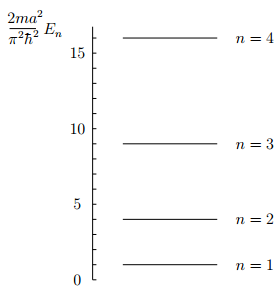
\includegraphics[scale=0.5]{img/image4.png}
		\captionof{figure}{Spectre d'une particule dans une boîte}
	\end{wrapfigure}
	En appliquant les conditions aux limites à l'équation différentielle résolue, on ne trouve pas de solution. Il n'y a pas d'état lié pour $E < 0$ car s'il existaient ils auraient une énergie cinétique négative (car pas d'EPot) ce qui n'a pas de sens.
	
	\subsubsection*{Pour $E > 0$}
	Cette fois-ci, on trouve des solutions acceptable ssi
	\begin{equation}
		ka = n\pi
	\end{equation}
	où $k = \sqrt{\frac{2mE}{\hbar^2}}$. Elle montre que seules certaines énergies sont acceptables. L'énergie est quantifiée (spectre quadratique) :
	\begin{equation}
		E_n = n^2 \frac{\pi^2\hbar^2}{2ma^2}
	\end{equation}
	où $n$ est appelé \textit{nombre quantique}.\\
	
	Les fonctions d'ondes correspondantes sont $C_1\sin(\pi n x/a)$ (comme $C_2 = 0$). On détermine $C_1$ à l'aide du premier postulat :
	\begin{equation}
		\int_0^a |C_1|^2\sin^2\left(\frac{\pi n x}{a}\right)dx = 1\ \ \ \Rightarrow\ C_1 = \sqrt{\frac{2}{a}}
	\end{equation}
	Notre fonction d'onde est ainsi :
	\begin{equation}
		\psi(x) = \sqrt{\frac{2}{a}}\sin\left(\frac{\pi n x}{a}\right)
	\end{equation}
	
	
	\section{Oscillateur harmonique}
	\subsection{Équation de Schrödinger en variables réduites}
	Considérons une particule de masse $m$ dans un potentiel $V(x) = \frac{1}{2}m\omega^2x^2$. L'équation de Schrödinger devient :
	\begin{equation}
		\left(-\frac{\hbar^2}{2m}\frac{d^2}{dx^2} + \frac{1}{2}m\omega^2x^2\right)\psi(x) = E\psi(x)
	\end{equation}
	
	Cette expression étant plus lourde que celle de la boîte, on va tenter de la simplifier grâce aux unités réduites, mais le prix à payer sera de perdre la cohérence dimensionnelle. Si $b$ est une longueur, $\hbar^2/mb^2$ et $m\omega^2b^2$ ont les dimensions d'une énergie.  Introduisons le \textit{paramètre d'oscillateur}:
	\begin{equation}
		b = \sqrt{\dfrac{\hbar}{m\omega}}
	\end{equation}
	ces énergies deviennent égales : $\hbar^2/mb^2 = m\omega^2b^2 = \hbar\omega$. Introduisons la variable sans dimension $u = x/b$ et la constante sans dimension $\epsilon = E/\hbar\omega$ et en posant $\phi(u) = \psi(bu)$ on obtient l'équation :
	\begin{equation}
		-\phi''(u) + u^2\phi(u) = 2\epsilon\phi(u)
	\end{equation}
	La solution approchée (WKB) est donnée par (retenir par cœur) :
	\begin{equation}
		\phi \sim e^{-u^2/2}
	\end{equation}
	En posant $\phi(u) = e^{-u^2/2}F(u)$ et en multipliant notre nouvelle équation par $e^{u^2/2}$ on trouve l'équation différentielle de Hermite :
	\begin{equation}
		F''(u) - 2uF'(u) + (2\epsilon - 1)F(u) = 0
	\end{equation}
	
	\subsection{Résolution par série de l'équation de Hermite}
	L'\textit{Annexe 6A} nous apprend qu'en développant en série autour de $u=0$ on peut trouver la forme valable $\forall  u$; On peut développer les solution sous la forme :
	\begin{equation}
		F(u) \equiv \sum_{j=0}^\infty a_ju^j = \sum_{j=-2}^\infty a_{j+2}u^{j+2}
	\end{equation}
	En remplaçant, on retrouve :
	\begin{equation}
		\sum_{j=-2}^\infty a_{j+2}(j+2)(j+1)u^j - 2\sum_{j=0}^\infty a_jju^j + (2\epsilon-1)\sum_{j=0} a_ju^j = 0
	\end{equation}
	En remarquant que les termes $j \leq 2$ sont nuls :
	\begin{equation}
		\sum_{j=0}^\infty\left[ (j+2)(j+1)a_{J+2} - 2ja_j + (2\epsilon - 1)a_j \right]u_j = 0 \forall u
	\end{equation}
	Pour que ceci fasse bien zéro, on obtient l'égalité suivante qui n'est rien d'autre que la \textit{relation de récurrence}:
	\begin{equation}\label{eq:5.21}
		(j+2)(j+1)a_{j+2} = (2j-2\epsilon+1)a_j
	\end{equation}
	Par récurrence, nous pouvons trouver deux solutions indépendantes :
	\begin{itemize}
		\item[$a_0 \neq 0, a_1 = 0$] : $a_0 \rightarrow a_2 \rightarrow a_4 \rightarrow ...$
		\item[$a_0 = 0, a_1 \neq 0$] : $a_1 \rightarrow a_3 \rightarrow a_5 \rightarrow ...$
	\end{itemize}
	Faire tendre $|u| \rightarrow \infty$ est équivalent à $j \rightarrow \infty$. Lorsque $j$ est grand, $j+1 \approx j$ et $2j-2\epsilon + 1 \approx 2j$. En divisant les deux membres par $j$, on trouve :
	\begin{equation}
		(j+2)a_{j+2} \approx 2a_j
	\end{equation}
	Lorsque $u$ est suffisamment grand, $F(u)$ est proportionnelle à une fonction $\sum_j \tilde{a}_ju^j$. En choisissant $\tilde{a}_0 \neq 0$ et $\tilde{a}_1 = 0$, la solution\footnote{Démonstration examen écrit!!} de \textbf{(5.22)} s'écrit en posant $j = 2k$ ou $2k+1$ (en remplaçant par $2k$, on retrouve le dev de l'exponentielle):
	\begin{equation}
		a_j \equiv \underbrace{a_{2k}}_{\underset{\underset{\text{par pas de 1}}{\text{varier $k$}}}{\text{Pour faire}}} \sim \frac{\tilde{a}_0}{k!} \Rightarrow F(u) \sim  \tilde{a_0}\sum_{k=0}^\infty \frac{u^{2k}}{k!} = \tilde{a_0}e^{u^2} \Rightarrow \phi(u) \sim \underbrace{\tilde{a_0}e^{u^2/2}}_{\underset{\underset{\text{car $j\rightarrow\infty$}}{\text{la solution}}}{\text{on tronque}}}
	\end{equation}
	Cette série converge vers une fonction divergente (la fonction d'onde se comporte comme une exp. croissante). N'étant pas physique, il faut la tronquer au cas ou il existe un nombre fini de $a_j \neq 0$, c'est à dire ou $F$ est un polynôme. Un coefficient $a_{n+2}$ peut être nul sans que le précédent ($a_n$) le soit si\footnote{Pour un certain $j$ que je vais appeler $n$, \eqref{eq:5.21} sera nulle et tout le reste suivra (sera aussi $=0$). Ce sera donc non nul jusque $n$ et nul après. Nous avons bien tronqué notre dev} :
	\begin{equation}
		2n-2\epsilon +1 = 0\  \ \ \ \ \ \Leftrightarrow\ \ \epsilon = n+\frac{1}{2}
	\end{equation}
	L'énergie étant définie par $\epsilon\hbar\omega$, celle-ci se retrouve quantifiée :
	\begin{equation}
		E_n = (n+\frac{1}{2})\hbar\omega
	\end{equation}
	L'énergie minimale correspond ici au cas ou $n=0$ (pour la boîte : $n=1$) et celle-ci vaut :
	\begin{equation}
		E_0 = \frac{1}{2}\hbar\omega
	\end{equation}
	
	
	\section{Barrière de potentiel constante}
	L'étude d'une particule non liée peut être faite grâce aux paquets d'ondes mais l'interprétation n'est pas facile. Étudions les états libres définis par $|\psi(x)|<\infty$ en considérant un potentiel de hauteur $V_0$ et de largeur $a$ :
	\begin{equation}
		V(x) = \left\{\begin{array}{ll}
			0 & x < 0\\
			V_0 & 0\leq x \leq a\\
			0 & x>a
		\end{array}\right.
	\end{equation}
	On effectuera une résolution par morceaux (le plus dur sera de "recoller" les morceaux).\\
	
	Soit le cas ou $E < V_0$ : la particule arrive de $x = -\infty$, arrive en 0, rebondit et reparte à vitesse opposée (en classique). En considérant le nombre d'onde :
	\begin{equation}
		K = \sqrt{\frac{2m(V_0 - E)}{\hbar^2}}
	\end{equation}
	Exprimé en équation de Schrödinger :
	\begin{equation}
		\left\{\begin{array}{lll}
			\dfrac{d^2\psi(x)}{dx^2} + \dfrac{2mE}{\hbar^2}\psi(x)  & \equiv \psi''(x) + k^2\psi(x) = 0 & x<0\ et\ a < x\\
			\dfrac{d^2\psi(x)}{dx^2} + \dfrac{2m(V_0-E)}{\hbar^2}\psi(x)  & \equiv \psi''(x) -K^2\psi(x) = 0 & 0 \leq x \leq a
		\end{array}\right.
	\end{equation}
	Qui résolut dans les trois régions de l'espace donne : 
	\begin{equation}
		\psi(x) = \left\{\begin{array}{ll}
			e^{ikx} + Re^{-ikx} & x<0\\
			A\sinh Kx + B\cosh Kx & 0\leq x \leq a\\
			Te^{ikx} + 0 & x > a
		\end{array}\right.
	\end{equation}
	où $R$ est le coefficient de réflexion et $T$, celui de transmission. L'absence d'une exponentielle décroissante dans le dernier terme suppose qu'il n'y a pas de particules allant vers la gauche au delà de $x=a$ et qu'aucune particule particule ne vient de $+\infty$. Nous avons également choisi un coefficient de normalisation de 1 pour $e^{ikx}$ afin d'avoir un état initial.\\
	
	Cette fonction d'onde $\psi(x)$ doit être continue sinon elle ne peut répondre à la définition de densité de probabilité. L'annexe $5A$ justifie que les dérivées premières doivent être continues.\\
	Exprimons la continuité de $\psi(x)$ et $\psi'(x)$ en $x=0$ et $x=a$ :
	\begin{equation}
		\left\{\begin{array}{l}
			1+R = B\\
			ik(1-R) = KA\\
			A\sinh Ka + B\cosh Ka = Te^{ika}\\
			K(A\cosh Ka + B\sinh Ka) = ikTe^{ika}
		\end{array}\right.
	\end{equation}
	En effectuant de jolis calculs, on peut trouver :
	\begin{equation}
		|T|^2 = \dfrac{4k^2K^2}{4k^2K^2 + v^4\sinh^2 Ka} \neq 0
	\end{equation}
	où $v^2 = \sqrt{\frac{2mV_0}{\hbar^2}}$. Un calcul similaire de $R$ montre la relation :
	\begin{equation}
		|R|^2 + |T|^2 = 1
	\end{equation}
	Cette relation implique que l'onde est ou réfléchie, ou transmise.\\
	
	Supposons que $Ka >> 1$, c'est à dire que $V_0 - E >> \frac{\hbar^2}{2ma^2}$ ce qui correspond à une large barrière ($a$ très grand), la probabilité de transmission peut être approchée par :
	\begin{equation}
		|T|^2 \approx \frac{16K^2}{v^4}k^2e^{-2Ka}
	\end{equation}
	Cette formule montre qu'il existe une probabilité non nulle de franchir une barrière
	« épaisse ». Cette probabilité décroît exponentiellement et peut être si petite que le
	phénomène ne soit jamais observé si $Ka$ est très grand, mais elle n'est pas nulle. Il y a donc une grande sensibilité à la largeur et à l'énergie.\\
	
	Notons que lorsque $E > V-0$ la particule ne se comporte pas exactement comme en classique. La probabilité de transmission est < 1, toutes les particules ne parviennent tout de même pas à la franchir (probabilité tout de même grande à  haute énergie).
	
	
	\section{L'effet tunnel}
	Le coefficient de transmission n'étant pas toujours calculable, on utilisera l'approximation $WKB$.\\
	
	L'effet tunel d'une barrière coulombienne joue un rôle important dans la fusion nucléaire. Grâce à l'effet tunnel, les étoiles peuvent fournir leur énergie progressivement et durant une longue durée.
	\begin{equation}
		|T|^2 \approx \exp(-2\pi\eta)
	\end{equation}
	où $\eta$ est le \textit{paramètre de Sommerfeld} (sans dimension) :
	\begin{equation}
		\eta = \frac{Z_1Z_2e^2}{4\pi\epsilon_0\hbar v}
	\end{equation}
	où $v$ est la vitesse relative $\sqrt{2E/\mu}$.\\
	
	Cette approximation de $|T|^2$ montre que la probabilité que deux noyaux fusionne à basse énergie décroît exponentiellement avec le produit de charges de ces noyaux. 
	Dans le soleil, seules les réactions où $Z_1Z_2 \leq 4$ ont lieu avec une probabilité suffisante.\\
	\chapter{Equations de Schrödinger à trois dimensions}
	\section{Potentiel central}
	Une particule de masse $m$ uniforme (postulat $IV$) \begin{equation}
		-\frac{\hbar^2}{2m}\Delta\psi(\vec r)+U(\vec r)\psi(\vec r)=E\psi(\vec r)
	\end{equation}
	Les fonctions d'ondes $\psi(\vec r)$ sont des fonctions propres bornées (postulat $I$) correspondant à certaines énergies propres $E$ de l'hamiltonien $H$ (postulat $III$)\\
	Fonctions d'onde bornées $\forall\vec r$:\begin{equation}
		\left|\psi(\vec r)\right|<\infty
	\end{equation}
	Pour obtenir des fonctions normées : $\int\left|\psi(\vec r)\right|^2\,d\vec r=1$, il faut chercher les solutions de carré sommable : $\int\left|\psi(\vec r)\right|^2\,d\vec r<\infty$\\\\
	Potentiel central = symétrie sphérique : 
	\begin{equation}
		V(r)=V(\|\vec r\|)
	\end{equation}
	ne dépendant que de $\|\vec r\|$. L'intérêt de ces potentiels sont que les interactions fondamentales de la nature sont \textit{invariantes par rotation}, d'intensité $=\forall$ directions.\\
	Ces potentiels sont eux aussi classable en confinant/non confinant ($C.f$ section~\ref{chap:5.1}).\\\\
	La différence avec les 1D : $V(\vec r)$ peut posséder une \textit{singularité à l'origine} (non borné en $r=0$ comme le potentiel coulombien). Nous supposons que $V$ vérifie :\begin{equation}
		\lim_{r\rightarrow 0}r^2V(r)=0
	\end{equation}
	ayant une singularité moins forte que $1/r^2$. Les potentiels sont donc continus à part à l'origine.\\\\
	On utilisera ici les coordonnées sphériques : $\left\{\begin{array}{l}
	x = r\sin\theta\cos\varphi\\
	y = r\sin\theta\sin\varphi\\
	z = r\cos\theta
	\end{array}\right.$
	\section{Le moment cinétique orbital}
	En mécanique classique, le moment cinétique est donné par $\vec L=\vec r\times\vec p : \left\{\begin{array}{l}
	L_x=yp_z-zp_y\\
	L_y=zp_x-xp_z\\
	L_z=xp_y-yp_x
	\end{array}\right.$
	Au niveau quantique, ceci se résume par : $\vec L=-i\hbar\vec r\times\vec\nabla$\\
	
	En coordonnées sphériques, l'opérateur $L_z$ devient : $L_z=-i\hbar\frac{\partial}{\partial\varphi}$ et l'opérateur $L^2$ est défini par $L^2=L^2_x+L_y^2+L_z^2$\\\\
	Grâce à l'annexe 6B : \begin{equation}
		L^2=-\hbar^2\left[\frac{1}{\sin\theta}\frac{\partial}{\partial\theta}\left(\sin\theta\frac{\partial}{\partial\theta}\right)\frac{1}{\sin^2\theta}\frac{\partial^2}{\partial\varphi^2}\right]
	\end{equation}
	ne dépendant que d'une dérivée en $\varphi$, l'expression de $L_z$ conduit à la relation de commutation :\begin{equation}
		[L^2,L_z]=0
	\end{equation}
	$\Rightarrow\exists$ ds fonctions propres communes à $L^2$ et $L_z$
	\section{Harmoniques sphériques}
	Les harmoniques sphériques constituent la base de l'espace des fonctions de carré sommable sur la sphère unité, $\in L^2([0,\pi]\times[0,2\pi])$. Ce sont les fonctions propres de carré du moment cinétique orbital et de sa composante en $z$.\\
	Comme ils commutent, $[L^2,L_z]\Rightarrow$ possède des fonctions propres en commun : \begin{equation}
		L^2Y_l^m(\theta,\varphi)=\hbar^2l(l+1)Y_l^m(\theta,\varphi)
	\end{equation}\begin{equation}
	L_zY^m_l(\theta,\varphi)=\hbar mY_l^m(\theta,\varphi)
\end{equation}\ \\
$\Rightarrow$ leurs valeurs propres font intervenir $\left\{\begin{array}{cl}
l & \text{: moment cinétique orbital} \rightarrow s(l=0),p(l=1)...\\
m & \text{: nombre quantique magnétique}
\end{array}\right.$
\begin{equation}
	-l\leq m\leq l\qquad \text{où }l\geq 0
\end{equation}
\danger $l$ n'est \textbf{PAS} la valeur propre de $\vec L$ ! $\rightarrow \vec L$ n'a pas de valeur propre et $L^2$ à comme valeur propre $\hbar^2l(l+1)$ \\\\
Les fonctions propres communes $L^2$ et $L_z$ := \textit{harmoniques sphériques} sont données par (annexes 6C et 6D)\begin{equation}
	Y_l^m(\theta,\varphi)=(-1)^{\frac{1}{2}(m+|m|)}\sqrt{\frac{2l+1}{4\pi}\frac{(l-|m|)!}{(l+|m|)!}}P_l^{|m|}(\cos\theta)e^{im\varphi}
\end{equation}
Les fonctions $P_l^{|m|}$ sont associées aux polynômes de Legendre (annexe 6E) : font apparaître le produit $\sin^{|m|}\theta$ et un polynôme de degré $(l-|m|)$ en $\cos\theta$ possédant $(l-|m|)$ zéros entre $\theta=0$ et $\theta=\pi$
\section{Séparation des variables}
Soit le Laplacien en coordonnées sphérique :\begin{align}
	\Delta & =\frac{1}{r}\frac{\partial^2}{\partial r^2}r-\frac{L^2}{\hbar^2r^2}\\
	& =\frac{\partial^2}{\partial r^2}+\frac{2}{r}\frac{\partial}{\partial r}-\frac{L^2}{\hbar^2r^2}
\end{align}
montrant que $\varphi$ et $\theta$ sont tous dans $L^2$. La séparation des variables est facile si les fonctions propres de $L^2$ sont connues.\\
Schrödinger devient\begin{equation}
	\left[-\frac{\hbar^2}{2m}\left(\frac{1}{r}\frac{\partial^2}{\partial r^2}r-\frac{L^2}{\hbar^2r^2}\right)+V(r)\right]\psi(\vec r)=E\psi(\vec r)
\end{equation}
Introduisons les solutions séparables : $\psi(\vec r)=Y^m_l(\theta,\varphi)R_l(r)$. L'action de $L^2$ sur ses fonctions propres et une division par $Y^m_l(\theta,\varphi)$ donne l'\textit{équation radiale}\begin{equation}
	\left[-\frac{\hbar^2}{2m}\left(\frac{1}{r}\frac{d^2}{dr^2}r-\frac{l(l+1)}{r^2}\right)+V(r)\right]R_l(r)=ER_l(r)
\end{equation}
Le nombre quantique magnétique $m$ à disparu et donc par valeur de $l \Rightarrow$ une équation radiale et pour certaines énergies $E$, une solution $R_l(r)$ := \textit{fonction d'onde d'onde radiale}. Le terme $\frac{1}{r}\frac{\partial^2}{\partial r^2}r=T_{radiale}$ et le terme $\frac{\hbar^2l(l+1)}{2mr^2}=T_{centrifuge}$\\

La résolution de Schrödinger se réduit à la recherche des valeurs propres et des fonctions propres de toutes les équations radiales.\\
Posons $u_l(r)=rR_l(r)$ : \begin{equation}
	\left[-\frac{\hbar^2}{2m}\left(\frac{d^2}{dr^2}-\frac{l(l+1)}{r^2}\right)+V(r)\right]u_l(r)=Eu_l(r)
\end{equation}
\ \\
où : 
\begin{equation}
	|R_l(r)|<\infty\ (\forall r)\qquad
	|u_l(r)|<\infty\ (\forall r)\qquad
	u_(0)=0
\end{equation}
Nous avons un problème de conditions aux limites auto-adjointes $\Rightarrow$ valeurs propres réelles (postulat $III$). On regroupe $T_{centrifuge}$ avec le potentiel : \begin{equation}\label{eq:6.14}
	\left(-\frac{\hbar^2}{2m}\frac{d^2}{dr^2}+V^l_{eff}(r)\right)u_l(r)=Eu_l(r)
\end{equation}
où $V_{eff}$ := \textit{potentiel effectif} : $\frac{\hbar^2}{2m}\frac{l(l+1)}{r^2}+V(r)$\\\\
Ceci ressemble fort au cas 1D \textbf{MAIS} doit satisfaire $u_l(0)=0$ qui $\nexists$ en 1D.\\
La normalisation de $\psi(\vec r)$ impose la normalisation des fonctions radiales $$\int_0^{\infty}[R_l(r)]^2r^2dr=1\qquad\int_0^{\infty}[u_l(t)]^2dr=1$$Remarque intéressante p87\\\\
L'équation de Schrödinger et $\psi(\vec r)=Y^m_l(\theta,\varphi)R_l(r)$ deviennent \begin{equation}
	\left(-\frac{\hbar^2}{2m}\Delta+V(r)\right)\psi_{n_rlm}(\vec r)=E_{n_rl}\psi_{n_rlm}(\vec r)
\end{equation}
et
\begin{equation}
	\psi_{n_rlm}(\vec r)=Y^m_l(\theta,\varphi)R_{n_rl}(r)=Y_l^m(\theta,\varphi)r^{-1}u_{n_rl}(r)
\end{equation}
Les valeurs propres éventuelles pour une valeur donné de $l$ vérifient \begin{equation}
	E_{0l}<E_{1l}<E_{2l}...
\end{equation}
L'état fondamental correspond à $l=0$, son énergie est notée $E_{00}$ ou $E_{0s}$.\\

Les fonctions d'onde sont des fonctions propres communes à $H$, $L^2$ et $L_z$. Les valeurs propres correspondantes sont $E_{n_rl}$, $\hbar^2l(l+1)$ et $\hbar m$\\
Les nombres quantiques qui caractérisent des valeurs propres qui commutent avec $H$ := \textit{bons nombres quantiques}
\section{Propriété générales des fonctions d'onde radiales}
Si $V(r)$ n'a pas d'autres singularité qu'à l'origine et à l'$\infty$, les solutions acceptables ont, près de l'origine, le comportement \begin{equation}
	u_l(r)\underset{{r\rightarrow 0}}{\backsim}r^{l+1}
\end{equation}\begin{equation}
R_l(r)\underset{{r\rightarrow 0}}{\backsim}r^l
\end{equation}
Comportement vérifié par toutes les fonctions d'onde radiales (ouf!). Ainsi, pour $l=0$, $R_0(r)$ ne converge \textbf{PAS} vers 0, c'est le seul cas où la densité de probabilité $|\psi(0)|^2\neq 0$\\\\
Comme le chapitre précédent, pour un potentiel confinant : \begin{equation}
	u_l(r)\underset{r\rightarrow\infty}{\backsim}\exp\left[-\frac{1}{\hbar}\int\sqrt{2mV(r)}dr\right]
\end{equation}
Pour un non confinant :\begin{equation}
	u_l(r)\underset{r\rightarrow\infty}{\backsim}\exp\left[\frac{1}{\hbar}\sqrt{2m|E|}r\right]
\end{equation}
Ces 3 équations sont les caractéristiques fondamentales de toutes les fonctions d'onde radiales.\\
Réécrivons \autoref{eq:6.14} : \begin{equation}
	\frac{u"_l}{u_l}=\frac{2m}{\hbar^2}(V_{eff}^l(r)-E)
\end{equation}
La courbure de la fonction radiale est $\propto V_{eff}^l(r)-E$ en ce point.\\

Choisissons le signe de $u_l(r)$ pour qu'elle soit $>0$ pour $r$ petit. Supposons \begin{equation}
	E<\underset{r}{min}\,V_{eff}^l(r)
\end{equation}
qui n'est possible que si $V^l_{eff}$ est borné inf $\Rightarrow u_l"$ a le même signe que $u_l'$. \\
Si $E>min\,V^l_{eff}(r)\rightarrow$ bien lire pp.90--91


\section{Potentiel coulombien attractif}
Comme nous l'indiquait notre devenu gentil cours de physique générale, le potentiel coulombien est défini par : 
\begin{equation}
	V(r) = -\frac{Ze^2}{4\pi\epsilon_0r}
\end{equation}

Insérons celui-ci dans l'équation de Schrödinger :
\begin{equation}
	\left(-\frac{\hbar^2}{2m_e}\Delta -\frac{Ze^2}{4\pi\epsilon_0r}\right)\psi(\vec{r}) = E\psi(\vec{r})
\end{equation}

Afin de traiter un problème plus simple, choisissons un système d'unité adapté (mais le prix à payer est la perte de la cohérence dimensionnelle) :
\begin{equation}
	\left\{\begin{array}{l}
		a_0 = 4\pi\epsilon_0\frac{\hbar^2}{m_ee^2} \\
		\text{Ryd} = \frac{\hbar^2}{2m_ea_0^2} = \frac{e^2}{8\pi\epsilon_0a_0}
	\end{array}\right.
\end{equation}
Ceci étant posé, effectuons le changement de variable :
\begin{eqnarray}
	\vec r \rightarrow \vec{r}a_0\\
	E \rightarrow E\ \text{Ryd}
\end{eqnarray}
où $\vec{r}$ et $E$ sont adimensionnel.\\

Après avoir effectué le changement de variable et divisé par Ryd, on trouve :
\begin{equation}
	\left(-\Delta - \frac{2Z}{r}\right)\psi(\vec r) = E\psi(\vec r)
\end{equation}

Comme vu au chapitre précédent, cherchons utilisons la séparation de variable $\psi_{n_rlm}(\vec r)=Y^m_l(\theta,\varphi)R_{n_rl}(r)$ combinée à $u_l(r)=rR_l(r)$ pour obtenir
\begin{equation}
	\left(-\frac{d^2}{dr^2} + \frac{l(l+1)}{r^2}-\frac{2Z}{r}\right)u_l(r) = Eu_l(r)
\end{equation}
dont nous allons chercher les solutions de carré sommable. Comme le potentiel tend vers zéro à l'infini, les seules solutions physiques correspondent à des énergies négatives; posons dès lors :
\begin{equation}
	\epsilon = \sqrt{-E}
\end{equation}
et aussi : 
\begin{equation}
	u_l(r) = e^{-\epsilon r} F_l(r)
\end{equation}
pour obtenir l'équation : 
\begin{equation}
	F_l'' - 2\epsilon F_l' - \frac{l(l+1)}{r^2}F_l + \frac{2Z}{r}F_l = 0
\end{equation}

Il s'ensuit d'une longue série de calculs. Comme ceux-ci ne sont pas matière d'examen de janvier, vous n'aurez ici droit qu'à un bref résumé des points clés :
\begin{itemize}
	\item Les solutions acceptables doivent avoir un comportement particulier à l’origine (Annexe 6A)
	\item En effectuant certains changements de variables proposés en annexe, on trouve une équation en série comme au Ch.5
	\item On peut en tirer (encore une fois, le raisonnement est similaire au chapitre précédent) une équation de récurrence :
	\begin{equation}
		j(j+2l+1)c_j = 2[\epsilon(j+l) - Z]c_{j-1}
	\end{equation}
	\item On peut montrer que cette équation peut se développer en série pour montrer que $u_l$ peut avoir pour comportement asymptotique : 
	\begin{equation}
		u_l(r) \backsim e^{+\epsilon r}
	\end{equation}
	\item Comme au Ch. précédent (oui, encore) ce n'est pas acceptable. Cependant, si un coefficient $c_j$ est nul tous les suivants le seront également et la soltuion sera acceptable physiquement. Ce sera le cas si :
	\begin{equation}
		\epsilon_n = \frac{Z}{n_r + l + 1} = \frac{Z}{n}
	\end{equation}
	\item Dans cette expression, $n$ est le \textit{nombre quantique principal} : $n = n_r + l + 1$.
	\item En rassemblant le tout, on trouve la formule de quantification de l'énergie :
	\begin{equation}
		E_n = -\frac{Z^2}{n^2} \text{Ryd}
	\end{equation}
\end{itemize}
La fin du chapitre montre comment à partir de cette quantification d'énergie on obtient le spectre discret de l'atome d'hydrogène mais également les fonctions d'ondes radiales de ce même atome ! A lire, bien évidemment ! (donc bien lire pp.94--98)



\chapter{Systèmes de particules}
\section{Équation de Schrödinger}
Le but est de généraliser la fonction d'onde à un système de $N$ particules, et donc à $3N$ dimensions dépendant du paramètre $t$ :
\begin{equation}
	\Psi(\vec{r_1}, \vec{r_2}, \dots, \vec{r_N}, t)
\end{equation}

Cette fonction d'onde reste bien déterminée par l'équation de Schrödinger 
\begin{equation}
	i\hbar\frac{\partial}{\partial t} \Psi(\vec{r_1}, \vec{r_2}, \dots, \vec{r_N}, t) = H \Psi(\vec{r_1}, \vec{r_2}, \dots, \vec{r_N}, t)
\end{equation}
où $H$ est l'opérateur hamiltonien. Quand celui-ci ne dépend pas du temps on retrouve la forme stationnaire
\begin{equation}
	H\Psi(\vec{r_1}, \vec{r_2}, \dots, \vec{r_N}, t) = E_T\Psi(\vec{r_1}, \vec{r_2}, \dots, \vec{r_N}, t)
\end{equation}
où $E_T$ est l'énergie totale du système. N'ayant plus une particule seule, il font considérer l'énergie cinétique et potentielle totale
\begin{equation}
	\left\{\begin{array}{ll}
		T &= \sum_{j=1}^N \frac{p_j^2}{2m_j} = - \sum_{j=1}^N \frac{\hbar^2}{2m_j}\Delta_j\\
		V &= \sum_{i>j=1}^N V_{ij}(|\vec{r_i}-\vec{r_j}|)
	\end{array}\right.
\end{equation}
où l'indice $j$ associé au gradient ou au laplacien signifie que l'opérateur différentiel porte sur la variable $\vec{r_j}$. L'opérateur énergie cinétique peut être vu comme une combili d'opérateurs laplaciens.\\
Pour le potentiel, la situation est idéalisée au cas ou le système est considéré comme seul dans l'espace : $V_{ij}$ est le potentiel d'interaction entre les particules $i$ et $j$. Ici on le considère central\footnote{$V_{ij} = V_{ji}$} et l'on ne porte attention qu'à la différence $|\vec{r_i}-\vec{r_j}|$. La condition $i>j$ permet d'éviter les doubles comptages.\\

Considérons par exemple le cas $N=2$ :
\begin{equation}
	i\hbar\Psi(\vec{r_1}, \vec{r_2},t) = \left[-\frac{\hbar^2}{2m_1}\Delta_1 - \frac{\hbar^2}{2m_2}\Delta_2 + V_{21}(|\vec{r_2}-\vec{r_1}|) \right]\Psi(\vec{r_1}, \vec{r_2},t)
\end{equation}
Cette fonction d'onde est définie dans un espace à 6 dimensions. Pour le cas $N=3$, la dimension de l'espace serait de 9.


\section{Interprétation de la fonction d'onde}
Il s'agit de considérer $N$ particules et non pus une seule comme précédemment. Supposons la fonction d'onde bornée :
\begin{equation}
	\int d\vec{r_1}\int d\vec{r_2}\dots\int d\vec{r_N}|\Psi(\vec{r_1}, \vec{r_2}, \dots, \vec{r_N}, t)|^2 = 1
\end{equation}
La normalisation se fait en intégrant sur les coordonnées de toutes les fonctions. Dans cette expression, la fonction 
\begin{equation}
	\rho(\vec{r_1}, \vec{r_2}, \dots, \vec{r_N}, t)=|\Psi(\vec{r_1}, \vec{r_2}, \dots, \vec{r_N}, t)|^2
\end{equation}
est la densité de probabilité de présence \textit{simultanée} des particules $i$ aux points $\vec{r_1}$. Il s'agit de la probabilité de trouver la particule 1 en position $\vec{r_1}$, la particule 2 en $\vec{r_2}$, ...\\
Si l'on souhaite uniquement avoir des informations sur la particule, on fera une intégrale de façon à ne garder que la particule en question
\begin{equation}
	\rho_1(\vec{r},t) = \int d\vec{r_2}\dots\int d\vec{r_N}\ \rho(\vec{r_1}, \vec{r_2}, \dots, \vec{r_N}, t)
\end{equation}
Cette expression est bien une densité de probabilité. La densité de probabilité de trouver une particule quelconque au point $\vec{r}$ est donné par la moyenne
\begin{equation}
	\rho^{(1)}(\vec{r},t) = \frac{1}{N}\sum_{j=1}^N \rho_j(\vec{r},t)
\end{equation}
dont l'intégrale sur tout l'espace est aussi égale à 1.

\section{Système de deux particules}
Dans \textbf{ce cas la}, on peut réaliser un équivalent quantique de la séparation du mouvement du centre de masse. L'équation de Schrödinger est celle rencontrée plus haut, mais dans le cas stationnaire :
\begin{equation}
	\left[-\frac{\hbar^2}{2m_1}\Delta_1 - \frac{\hbar^2}{2m_2}\Delta_2 + V_{21}(|\vec{r_2}-\vec{r_1}|) \right]\Psi(\vec{r_1}, \vec{r_2},t) = E_T \Psi(\vec{r_1}, \vec{r_2},t)
\end{equation}
où $E_T$ est l'énergie totale. Définissions la \textit{coordonnée du centre de masse} comme en \textit{Mécanique Rationnelle I}
\begin{equation}
	\vec{R} = \frac{m_1\vec{r_1}+m_2\vec{r_2}}{M}
\end{equation}
où $M$ est la masse totale. Définissions la \textit{coordonnée relative} $\vec{r} = \vec{r_1}-\vec{r_2}$ ainsi que la masse réduite :
\begin{equation}
	\frac{1}{\mu} = \frac{1}{m_1}+\frac{1}{m_2}
\end{equation}

Notre équation devient 
\begin{equation}
	\left[- \frac{\hbar^2}{2M}\Delta_{\vec{R}} - \frac{\hbar^2}{2\mu}\Delta_{\vec{r}} + V(r) \right]\Psi(\vec{R}, \vec{r}) = E_T \Psi(\vec{R}, \vec{r})
\end{equation}
On y voit apparaître :
\begin{enumerate}
	\item L'énergie cinétique du centre de masse du système ou la masse peut être vue comme celle d'une "particule virtuelle".
	\item L'énergie cinétique et potentielle relative des deux particules
\end{enumerate}

Grâce à ces nouvelles variables, on peut appliquer la méthode de séparation des variables pour factoriser $\Psi$ comme
\begin{equation}
	\Psi(\vec{R},\vec{r}) = e^{i\vec{K}.\vec{R}}\varphi(\vec{r})
\end{equation}
où $\vec{K}$ est le vecteur d'onde décrivant le mouvement du centre de masse\footnote{Comme en classique, le centre de masse effectue un MRU de vitesse $\hbar\vec{K}/M$.}. L'énergie totale est ainsi la somme de l'énergie du centre de masse additionné à celle des particules : $E_T = E_{CM} + E$.\\

La \textit{fonction d'onde du mouvement relatif $\varphi(\vec{r})$} est la solution de l'équation de Schrödinger du mouvement relatif\footnote{Sa résolution donne la partie "interne" de l'énergie.} :
\begin{equation}
	\left[-\frac{\hbar^2}{2\mu}\Delta_{\vec{r}} + V(r)\right]\varphi(\vec{r}) = E\varphi(\vec{r})
\end{equation}
où \textit{l'énergie $E$ du mouvement relatif} est reliée à l'énergie totale par la relation 
\begin{equation}
	E = E_T - \frac{\hbar^2K^2}{2M}
\end{equation}
Pour étudier un système de deux particules, il suffit de calculer leur masse réduite et d'écrire l'équation de Schrödinger associée (après la résoudre est moins rigolo).


\section{L'atome d'hydrogène}
Soit un système d'un électron de masse $m_e$ de charge $-e$ et d'un proton de masse $m_p$ de charge $e$. En écrivant directement la fonction d'onde du mouvement relatif, on trouve
\begin{equation}
	\left(-\frac{\hbar^2}{2\mu}\Delta - \frac{e^2}{4\pi\varepsilon_0 r}\right)\varphi(\vec{r}) = E\varphi(\vec{r})
\end{equation}
Ce qui ressemble fort à l'équation de Schrödinger en 3D dans un potentiel coulombien (où $Z=1$) si ce n'est que la masse de la "particule" est\footnote{Approximation au premier ordre autour de 0.}
\begin{equation}
	\mu = \frac{m_em_p}{m_e+m_p} \approx m_e\left(1-\frac{m_e}{m_p}\right)
\end{equation}
où le rapport $\frac{m_e}{m_p} \approx \frac{1}{1836}$.\\
L'équation de Schrödinger ressemblant fortement à celle du Ch6, on peut trouver ses solutions par analogies. Définissions les unités effectives :
\begin{equation}
	\left\{\begin{array}{lll}
		a_\mu &= 4\pi\epsilon_0 \dfrac{\hbar^2}{\mu e^2} &= \dfrac{m_e}{\mu}\ a_0\\
		\text{Ryd}_\mu &= \dfrac{e^2}{8\pi\epsilon_0a_\mu} &= \dfrac{\mu}{m_e}\ \text{Ryd}
	\end{array}\right.
\end{equation}
Ceci considère intuitivement que quand on considère que le mouvement du proton a deux effets :  le système à tendance à devenir un peu plus large (il se détend vu que comme il peut bouger il prend plus de place)
et, par son déplacement, il sera un peu plus "mou" ce qui justifie une diminution d'énergie.\\

Grâce aux unités effectives, on retrouve exactement la forme trouvée au chapitre précédent et forcement, le spectre d'énergie d'un atome d'hydrogène est donné par\footnote{C'est d'ailleurs une très bonne approximation !} :
\begin{equation}
	E_n = -\frac{1}{n^2}\text{Ryd}_\mu \approx -\frac{1}{n^2}\left(1-\frac{m_e}{m_p}\right)\ \text{Ryd}
\end{equation}

\section{Systèmes hydrogénoïdes}
Un système \textit{hydrogénoïde} est un système composé de deux particules de charges opposées qui n'interagissent que par l'interaction coulombienne. En pratique, ces systèmes comportent une particule de charge $-e$ et une autre de charge $Ze\ (Z \geq 1)$. Ces systèmes ont une énergie quantifiée :
\begin{equation}
	E_n = -\frac{Z^2}{n^2}\text{Ryd}_\mu
\end{equation}

Un bel exemple est le \textit{positronium}, constitué d'un électron et de son anti-particule ; le positron. Ayant exactement la même masse, la masse réduite est ici exacte et vaut
\begin{equation}
	\mu = \frac{1}{2}m_e
\end{equation}

\section{État de Rydberg}
L'expression $E_n = -\frac{Z^2}{n^2}\text{Ryd}_\mu$ reste valable pour de très grandes valeurs de $n$ ; les états très excités de l'atome d'hydrogène sont les \textit{états de Rydberg}\footnote{En excitant progressivement les atomes d'hydrogène avec un laser.}. Lorsqu'on a un tel $n$, $l=n-1$ est de grande dimension, on a alors:
\begin{equation}
	<r>_{nn-1} \approx n^2a_0
\end{equation}
Pour $n\approx 500$, le rayon moyen de ces états est de l'ordre de grandeur de $0,01\ mm$!

\section{Systèmes de particules identiques}
Tous les électrons sont identiques entre eux, considérer un système de $n$ particules différentes n'a qu'un intérêt limité ; systèmes à deux ou trois corps ont inévitablement plusieurs fois la même particule. Lorsque deux particules identiques sont proches l'une de l'autre, on ne pourra plus les identifier car elles ont toutes les deux une probabilité de présence non nulles en les mêmes points, c'est le \textit{principe d'indiscernabilité}.\\

Considérons deux particules identiques 1 et 2 dont l'hamiltonien est donné par :
\begin{equation}
	H(1,2) = T(1)+T(2) + V(1,2)
\end{equation}
où $T(1)$ et $T(2)$, les opérateurs d'énergie cinétique, ont la même forme car les particules ont la même masse ; ils ne diffèrent que par leur coordonnée, dépendant de 1 ou 2. Le potentiel d'interaction est lui aussi symétrique :
\begin{equation}
	V(1,2) = V(2,1)
\end{equation}
Il en résulte que l'hamiltonien est symétrique $H(1,2) = H(2,1)$. Considérons-en une fonction propre :
\begin{equation}
	H(1,2)\Psi(1,2) = E\Psi(1,2)
\end{equation}
Les valeurs propres ne sont en général pas dégénérées. On a également, en permutant 1 et 2 :
\begin{equation}
	H(2,1)\Psi(2,1) = E\Psi(2,1)
\end{equation}
Comme $H$ est ici symétrique $H(1,2)\Psi(2,1) = E\Psi(2,1)$. On voit que $\Psi(1,2)$ et $\Psi(2,1)$ sont fonctions propres du même opérateur avec la même valeur propre ; comme l'énergie n'est pas dégénérée, $\Psi(2,1)$ doit être proportionnel à $\Psi(1,2)$ :
\begin{equation}
	\Psi(2,1) = C\Psi(1,2)
\end{equation}
En permutant les indice $\Psi(1,2) = C\Psi(2,1)$. En remplaçant l'une dans l'autre :
\begin{equation}
	\Psi(2,1) = C^2\Psi(1,2)
\end{equation}
La fonction propre étant normée, on a donc obligatoirement $C = \pm 1$ ce qui signifie que $\Psi$ est soit symétrique, soit antisymétrique :
$\left\{\begin{array}{ll}
\text{Symétrique} &\Leftrightarrow \Psi_S(2,1) = \Psi_S(1,2)\\
\text{Antiymétrique} &\Leftrightarrow \Psi_S(2,1) = -\Psi_S(1,2)
\end{array}\right.$.\\
Un théorème non démontré ici (théorie des groupes) dit que les fonctions propres sont soit complètement symétrique, soit complètement antisymétrique. Les densité de probabilités seront par contre toujours symétriques. Cet effet symétrique n'est pas observable directement, mais cause des effets indirects importants.

\subsection{Postulat d'antisymétrisation de Pauli}
\textit{Les états physiques d'un système de particules identiques qui sont soit des électrons, soit des protons, soit des neutrons sont décrits par des fonctions d'ondes antisymétriques.}\\
Même si des solutions mathématiques symétriques existent, elles sont dénuées de sens physique.\\

De ce postulat découle le principe d'exclusion de Pauli : la probabilité d'avoir deux particules au même endroit est nulle :
\begin{equation}
	\Psi_A(\vec{r_1},\vec{r_1}) = -\Psi_A(\vec{r_1},\vec{r_1}) = 0
\end{equation}
Ceci explique la structure en couche des atomes. Les fonctions d'ondes complètement antisymétriques porte le doux nom de \textit{fermions}. Cf. slide 12/13 \& syllabus page 112/113 pour plus d'infos !



\chapter{Le spin}
\section{L'effet Zeeman anormal}
Le moment magnétique associé au mouvement de l'électron est donné par $\vec{M_L} = 
-\frac{e}{2m_e}\vec{L}$. Si on plonge l'$e^-$ dans un champ $\vec{B}$, il apparaît
une énergie potentielle d'interaction $W = -\vec{M_L}.\vec{B}$ modifiant l'
hamiltonien\footnote{Choisi ici dans la direction $z$ mais cela ne change rien.} :
\begin{equation}
	H \rightarrow \tilde{H} = H + \frac{e}{2m_e}BL_z
\end{equation}
Les fonctions propres de $\tilde{H}$ restent les même qu'aux chapitre 6, mais les 
énergies deviennent :
\begin{equation}
	E_n \rightarrow \tilde{E}_{nm} = -\frac{1}{n^2}\text{Ryd} + \mu_BBm
\end{equation}
où $l$ est le nombre quantique magnétique et $\mu_B = \frac{e\hbar}{2m_e} \approx
9.29\times 10^{-24} J/T$ le magnéton de Bohr.\\
On voit que l'énergie dépend maintenant du nombre quantique magnétique $m$ impliquant
qu'un niveau d'énergie $E_n$ se subdivise en plusieurs niveaux d'énergies différentes
$\tilde{E}_{mn}$ :
\begin{equation}
	1\ \text{niveau} \rightarrow 2l + 1\ \text{niveaux}
\end{equation}
Le nombre de niveau devrait être alors impair, mais cette propriété n'est pas toujours
vérifiée par l'expérience ; il faudrait que $j$ soit \textit{demi-entier.}

\section{L'expérience de Stern et Gerlach}
Le but de cette expérience est de mesurer les moments magnétiques d'atomes neutres\footnote{
	afin d'éviter que la force de Lorentz ne les dévie.}. Si le champ d'induction est
homogène, le potentiel correspondra à une force non nulle $\vec{F} = \vec{\nabla}(
\vec{M_L}.\vec{B})$ capable de dévier verticalement les atomes possédant un moment 
magnétique.\\
Les moments magnétiques étant supposés \^etre aléatoires, l'expérience devrait faire
appara\^itre une tache mais ce n'est pas le cas : on peut voir apparaître plus d'une
tache impliquant la quantification du moment cinétique. Ce problème sera résolu en 
introduisant la notion de \textit{spin}\footnote{A prononcer s-pain pour être certain
	que l'oral se passe bien.}.

\section{Le spin}
On a proposé d'associer à l'électron, en 1926, un moment cinétique non entier appelé
\textit{spin} valant $1/2$, c'est-à-dire un demi quantum de moment cinétique $\hbar/
2$.\\
Il s'agit d'une propriété \textbf{intrinsèque} à la particule et donc totalement 
différent du moment cinétique orbital qui est du au mouvement de celle-ci (et qui 
a après été associé à toutes les particules et non seulement l'électron).\\
Rappelons nous les commutateurs des composantes de $\vec{L}$ :
\begin{equation}
	\begin{array}{ll}
		[L_x,L_y]            & = i\hbar L_z \\
		\left[L_y,L_z\right] & = i\hbar L_x \\
		\left[L_z,L_x\right] & = i\hbar L_y 
	\end{array}
\end{equation}
sans oublier que $L^2$ et $L_z$ commutent (et comme l'axe $z$ n'a rien de particulier,
c'est aussi le cas pour $L_x$ et $L_y$). D'autres opérateurs vérifient-t-ils ces 
relations? \\
Soit le moment cinétique de spin $\vec{S} = (S_x,S_y,S_z)$ aux propriétés analogues
à $\vec{L}$ :
\begin{equation}
	\begin{array}{cc}
		[S_x,S_y]            & = i\hbar S_z \\
		\left[S_y,S_z\right] & = i\hbar S_x \\
		\left[S_z,S_x\right] & = i\hbar S_y 
	\end{array}
\end{equation}
On peut vérifier par calcul direct que ces trois relations sont vérifiées par les 
trois \textit{matrices de Pauli} (qui forment une base de l'espace vectoriel des 
matrices $2\times2$ hermétiques avec la matrice unité)
\begin{equation}
	S_k = \frac{\sigma_k \hbar}{2}\ \ \ \ (k=x,y,z)
\end{equation}
avec
\begin{equation}
	\sigma_x = \left(\begin{array}{cc}
		0 & 1\\
		1 & 0
	\end{array}\right),\ \ \ \ \ \sigma_y =	\left(\begin{array}{cc}
	0 & -i\\
	i & 0
\end{array}\right),\ \ \ \ \ \sigma_z =	\left(\begin{array}{cc}
1 & 0\\
0 & -1
\end{array}\right)
\end{equation}
On vérifie facilement que $\sigma_x^2 = \sigma_y^2 = \sigma_z^2 = \mathcal{I}$ mais
aussi que :
\begin{equation}
	\begin{array}{lll}
		\sigma_x\sigma_y & = -\sigma_y\sigma_x = i\sigma_z, \\
		\sigma_y\sigma_z & = -\sigma_z\sigma_y = i\sigma_x, \\
		\sigma_z\sigma_x & = -\sigma_x\sigma_z = i\sigma_y  
	\end{array}
\end{equation}
Par analogie au chapitre 6, définissions $S^2 = S_x^2 + S_y^2 + S_z^2$. On trouve
alors que $S^2 = \frac{3}{4}\hbar^2\mathcal{I}$.\\

Comme $S^2$ et $S_z$ commutent, elles sont des vecteurs propres en communs qui sont :
\begin{equation}
	\chi_{+1/2} = \left(\begin{array}{cc}
		1\\
		0
	\end{array}\right),\ \ \ \ \ \	\chi_{-1/2} = \left(\begin{array}{cc}
	0\\
	1
\end{array}\right)
\end{equation}
Et, toujours par analogie, on peut alors écrire :
\begin{eqnarray}
	S^2\chi_{m_s} = \hbar^2 s(s+1)\chi_{m_s},\\
	S_z\chi_{m_s} = \hbar m_s\chi_{m_s}
\end{eqnarray}
avec $s = \frac{1}{2}$ et $m_s = \pm \frac{1}{2}$. L'opérateur $S^2$ possède une 
valeur propre $3\hbar^2/4$ doublement dégénérée correspondant à un nombre quantique
$s=1/2$ ; il existe $2s+1=2$ états différents correspondant à cette valeur propre 
donnant deux vecteurs propres orthogonaux.\\

Les deux expériences introductives du chapitre montrent que l'électron peut exister
dans deux états différents $\chi_{+1/2}$ et $\chi_{-1/2}$ et qu'il possède un 
moment magnétique supplémentaire appelé \textit{moment magnétique intrinsèque} :
\begin{equation}
	\vec{M_S} = -g_e\frac{e}{2m_e}\vec{S}
\end{equation}
où $g_e \approx 2$. Le moment magnétique total de l'électron est alors donné par :
\begin{equation}
	\vec{M} = \vec{M_L}+\vec{M_S} = -\frac{\mu_B}{\hbar}(\vec{L}+g_e\vec{S})
\end{equation}
L'énergie potentielle d'interaction de l'électron avec le champ d'induction $\vec{B}$
doit être remplacée par $W = -\vec{M}.\vec{B}$ qui permet d'expliquer les 
contradictions montrées en début de chapitre.


\section{Propriétés générales d'un moment cinétique}
Un \textit{moment cinétique} $\vec{J} = (J_x,J_y,J_z)$ est un \textit{opérateur 
	vectoriel} comportant trois composantes hermétiques qui vérifient les \textit{ 
	relations de commutations}. Le carré du moment cinétique est défini par $J^2 = 
J_x^2 + J_y^2 + J_z^2$. \\
Si on définit un moment cinétique comme tel, on peut démonter qu'il vérifie un 
certain nombre de propriétés comme le fait que les opérateurs $J^2$ et $J_z$
possèdent des fonctions propres communes $\psi_{jm}$ telles que :
\begin{equation}
	\begin{array}{ll}
		J^2\psi_{jm} & = \hbar^2 j(j+1)\psi_{jm} \\
		J_z\psi_{jm} & = \hbar m \psi_{jm}       
	\end{array}
\end{equation}
Les nombres quantiques $j$ et $m$ vérifient les trois propriétés suivantes :
\begin{enumerate}
	\item $j$ est positif, entier ou demi entier ; $j \in \{0,1/2,1,3/2,\dots \}$
	\item $m$ peut prendre $2j+1$ valeurs ; $-j\leq m \leq j$
	\item $j+m$ est entier ; $j+m \in \mathbb{N}$
\end{enumerate}
\textbf{Attention !} Il est important de ne pas confondre l'opérateur de 
moment cinétique $\vec{J}$ et le nombre quantique de moment cinétique $j$ !

\section{Composition de deux moments cinétiques}
Si on s'intéresse à ces propriétés, c'est parce qu'il existe de nombreuses sortes
de moments cinétiques qui ont la propriété suivante : \textit{la somme de deux 
	moments cinétiques est un moment cinétique}.\\
Soit $\vec{J_1},\vec{J_2}$, deux moments cinétiques indépendants dont leur 
somme est $\vec{J} = \vec{J_1}+\vec{J_2}$. Ils vérifient bien les propriétés
du commutateurs. Par exemple :
\begin{equation}
	\begin{array}{ll}
		[J_x,J_y] & = [J_{1x}+J_{2x},J_{1y}+J_{2y}]                                                    \\
		& = \left[J_{1x},J_{1y}\right]+\left[J_{1x},J_{2y}\right]+\left[J_{2x},J_{1y}\right] 
		+\left[J_{2x},J_{2y}\right]\\
		& = i\hbar J_{1z } + 0 + 0 + i\hbar J_{2z}                                           \\
		& = i\hbar J_{z}                                                                     
	\end{array}
\end{equation}
Ceci à pour conséquence que toutes les propriétés vues à la section 8.4 sont 
valables ici : il doit exister une relation reliant le nombre quantique $j$ à
la valeur propre $\hbar^2j(j+1)$ de l'opérateur $J^2$. On peut démontrer que 
ces trois nombres vérifient :
\begin{equation}
	|j_1-j_2| \leq j \leq j_1+j_2\ \ \ \ \ \text{et }\ \ j_1+j_2+j_3\ \ \text{entier}
\end{equation}
Il s'agit des \textit{relations triangulaires}. Notons que les côtés de ces 
"triangles quantiques" sont contraints par les valeurs de $j$. On peut donc 
avoir deux possibilités :
\begin{enumerate}
	\item $j$ entier
	\begin{itemize}
		\item Si $j_1$ et $j_2$ entiers
		\item Si $j_1$ et $j_2$ demi-entiers
	\end{itemize}
	\item $j$ demi-entier
	\begin{itemize}
		\item Si $j_1$ entier et $j_2$ demi-entier
		\item Si $j_1$ demi-entier $j_2$ entier
	\end{itemize}
\end{enumerate}


\section{Moment cinétique orbital}
Le \textit{moment cinétique total d'un électron} est défini par : $\vec{J} = 
\vec{L}+\vec{S}$. D'après les relations quantiques, le nombre quantique $j$ 
correspondant à la valeur propre $\hbar^2j(j+1)$ ne prend que des valeurs demi-
entières :
\begin{equation}
	\left|l-\frac{1}{2}\right| \leq j \leq l+\frac{1}{2}\ \ \ \ \Leftrightarrow\ \ \ \
	j = \left|l\pm\frac{1}{2}\right|
\end{equation}
Les propriétés sur les nombres quantiques imposent que les valeurs de $m$ soient
également demi-entière et vérifient :
\begin{equation}
	m = -j, -j+1, -j+2, \dots, j-2,j-1,j
\end{equation}
Par exemple, pour $j=3/2$, les valeurs de $m$ sont $-3/2,-1/2,1/2,3/2$ qui sont 
bien au nombre de $2j+1=4$.\\

Le \textit{moment cinétique total} est la somme des moments cinétiques de toutes 
les particules d'un système :
\begin{equation}
	\vec{J} = \sum_{i=1}^N\vec{J_i} = \sum_{i=1}^N \vec{L_i} + \sum_{i=1}^N \vec{S_i}
\end{equation}
\textbf{Attention !} Il s'agit bien d'opérateur qui s'additionnent "simplement", à 
ne pas confondre avec les nombres quantiques qui ont des \textit{lois de composition} 
plus compliquées données par les relations triangulaires.


\section{La structure fine de l'atome d'hydrogène}
Le spin impliquant de nouvelles propriétés comme la subdivision du spectre appelées 
\textit{structure fine} : il faut reconsidérer l'étude de l'atome d'hydrogène.\\
Considérons un électron (avec spin) dans un potentiel coulombien du à la présence 
d'un proton (sans spin) : l'équation de Schrödinger est toujours valable, mais il 
faut modifier l'hamiltonien et les fonctions d'ondes pour tenir compte du spin.\\
Les fonctions d'ondes deviennent : 
\begin{equation}
	\psi_{nlm_lm_s}(\vec{r}) = Y_l^{m_l}(\theta,\varphi)R_{nl}(r)\chi_{m_s}
\end{equation}
Ou, plus explicitement :
\begin{equation}
	\begin{array}{ll}
		\psi_{nlm_l,1/2}(\vec{r}) & = \left(\begin{array}{cc} 
			Y_l^{m_l}(\theta,\varphi)R_{nl}(r)\\
			0
		\end{array}\right),\\
		& \\
		\psi_{nlm_l,-1/2}(\vec{r}) &= \left(\begin{array}{cc}
			0\\
			Y_l^{m_l}(\theta,\varphi)R_{nl}(r)
		\end{array}\right)
	\end{array}
\end{equation}
Chaque fonction d'onde est devenue un vecteur-colonne à deux composantes que l'on 
nomme \textit{spineur}. Si $H_0$ est l’hamiltonien dans l'équation de Schrödinger,
on peut associer à notre nouvelle fonction d'onde un hamiltonien matriciel :
\begin{equation}
	\mathcal{H}_0 =\left(\begin{array}{cc}
		H_0 & 0\\
		0 & H_0
	\end{array}\right)
\end{equation}
La vitesse quadratique moyenne d'un électron dans un état de nombre quantique 
principal $n$ est donnée par :
\begin{equation}
	\sqrt{\langle v^2\rangle_n} = \alpha c/n
\end{equation}
où $\alpha = \frac{e^2}{4\pi\epsilon_0\hbar c}	 \approx \frac{1}{137}$ est la \textit{
	constante de structure fine} qui mesure l'intensité de la constante d'interaction 
coulombienne $e^2/4\pi\epsilon_0$.\\

Les corrections relativistes conduisent à modifier $\mathcal{H}_0$ en $\mathcal{H} = 
\mathcal{H}_0 + \mathcal{V}_{LS} + \dots$ où l'on voit un "potentiel" dépendant du 
spin :
\begin{equation}
	\mathcal{V}_{LS} = V_{LS}(r)\ \vec{L}.\vec{S}
\end{equation}
d'ordre de grandeur $\alpha^2\text{Ryd}$. Ce terme est le \textit{couplage spin-
	orbite}. L'opérateur responsable du couplage spin-orbite s'écrit : 
\begin{equation}
	\vec{L}.\vec{S} = L_xS_x + L_yS_y + L_zS_z\ = \frac{1}{2}\hbar\left(\begin{array}{cc}
		L_z & L_x-iL_y\\
		L_x+iL_y & -L_z
	\end{array}\right)
\end{equation}
Les spineurs ne sont pas des fonctions propres de $\mathcal{H}$ sauf pour les états
$s$. Pour les états $l\neq 0$ les fonctions propres de $\mathcal{H}$ sont plus 
compliquées : elles sont combili des spineurs $\rightarrow$ ce sont donc aussi des
fonctions propres de $L^2$ et de $S^2$ et donc les spineurs que l'on recherche sont 
aussi fonctions propres de l'opérateur 
\begin{equation}
	J^2 = (\vec{L}+\vec{S})^2 = L^2 + S^2 + 2\vec{L}.\vec{S}
\end{equation}
Ces spineurs sont aussi fonctions propres de $J_z = L_z+S_z$ qui commute avec $\vec{
	J}$ \textbf{et} $\vec{L}.\vec{S}$ : il est pratique d'utiliser $j$ et $m$ pour 
caractériser les états propres de $\mathcal{H}$ qui sont notés $\psi_{nljm}(\vec{r})$.\\

Les fonctions propres de $\mathcal{H}$ peuvent être calculées par un \textit{calcul 
	des perturbations} dont les énergies des états $nlj$ sont données par 
\begin{equation}
	E_{nlj} = \left[-\frac{1}{n^2} - \frac{\alpha^2}{n^4}\left(\frac{n}{j+\frac{1}{2}}-
	\frac{3}{4}\right)\right]\ \text{Ryd}_\mu
\end{equation}
où le premier terme est habituel et le second est la correction de structure fine, 
d'ordre $\alpha^2$.\\
La structure fine ne dépendant que de $j$ les états de m\^eme $j$ comme $2s1/2$ et $2p1/2$ 
devraient avoir	la m\^eme énergie mais ce n'est pas le cas expérimentalement. Ceci 
est du aux \textit{déplacement de Lamb} d\^u à la \textit{polarisation du vide} :
une interaction entre un état d'un système de particules chargées et les photons qui 
transmettent le champ électromagnétique entre les particules.

\section{La structure hyperfine de l'atome d'hydrogène}
Si l'on tient compte du spin du proton, le spectre se subdivise encore pour obtenir
la structure \textit{hyperfine}. Le facteur gyromagnétique pour le proton vaut $
g_p \approx 5.6 \neq 2$ car ce n'est pas une particule élémentaire. Le moment 
magnétique intrinsèque du proton est :
\begin{equation}
	\vec{M_S} = g_p \frac{e}{2m_p}\vec{S_p}
\end{equation}
qui est beaucoup plus faible que celui de l'électron à cause de la grande masse du
proton. La présence d'un potentiel hyperfin (non détaillé ici) conduit à un moment
cinétique supplémentaire $\vec{F}=\vec{J}+\vec{I}$ (moment total de l'électron +
spin du proton). Comme $I = 1/2$, on retrouve :
\begin{equation}
	F = \left|j\pm\frac{1}{2}\right|
\end{equation}








\chapter{Les atomes}
\section{La physique atomique}
Dans un noyau, la masse $m_e$ des électrons est beaucoup plus faible que celle du
noyau $M$. Ce dernier possède un rayon $\approx 10^{-15}\ m$. Si $Z \neq N$, l'
atome est un \textit{ion} ; chargé positivement si $Z>N$ et négativement dans l'
autre cas. Dans ce chapitre, on ne considérera que des atomes neutres $Z=N$ et le
noyau sera vu de façon ponctuelle.

\section{L'atome d'hélium}
\subsection{Équation de Schrödinger}
En négligent les effets (hyper)fins, la fameuse équation de ce système à trois 
particules s'écrit :
\begin{multline}
	\left[-\frac{\hbar^2}{2M}\Delta_N-\frac{\hbar^2}{2m_e}\Delta_1-\frac{\hbar^2}{2m_e}\Delta_2\right.\\
	\left.+\frac{e^2}{4\pi\epsilon_0} \left(-\frac{Z}{|\vec{r_N}-\vec{r_1}|}-\frac{Z}{|\vec{r_N}-
		\vec{r_2}|}+\frac{1}{|\vec{r_1}-\vec{r_2}|}\right)\right]\psi(\vec{r_N},\vec{r_1},\vec{r_2}) = 
	E\psi(\vec{r_N},\vec{r_1},\vec{r_2})
\end{multline}
où $\vec{r_N}$ est la coordonnée du noyau et $\vec{r_1},\vec{r_2}$ les coordonnées 
des deux électrons. On peut éliminer le mouvement du centre de masse - ce qui est
une bonne approximation - en faisant tendre $M \rightarrow \infty$ afin que le 
noyau devient un "point fixe" de coordonnée $\vec{r_N}=\vec{0}$. On décrit alors 
l'atome par l'hamiltonien :
\begin{equation}
	H = H_1+H_2+V_12\ \ \text{où}\ \ \left\{\begin{array}{ll}
		H_j &= \frac{p_j^2}{2m_e}-\frac{Ze^2}{4\pi\epsilon_0r_j}  \\
		V_{12} &= \frac{e^2}{4\pi\epsilon_0|\vec{r_1}-\vec{r_2}|} 
	\end{array}\right.\ \ (i=1,2), \vec{p_j}=-i\hbar\vec{\nabla_j}
\end{equation}


\subsection{Étude qualitative du spectre de l'atome d'hélium}
Pour commencer cool, on considère un hamiltonien peu réaliste mais beaucoup plus
simple : $\tilde{H} = H_1+H_2$. Comme chacun des termes ne dépend que d'une 
seule variable, les fonctions propres de $\tilde{H}$ sont de la forme :
\begin{equation}
	\tilde{\psi}(\vec{r_1},\vec{r_2}) = \psi_{n_1l_1m_1}(\vec{r_1})\psi_{n_2l_2m_2}(
	\vec{r_2})
\end{equation}
En évaluant sont produit avec $\tilde{H}$ et en appliquant la définition faisant
apparaître les valeurs propres : 
\begin{equation}
	\begin{array}{ll}
		\tilde{H}\tilde{\psi}(\vec{r_1},\vec{r_2}) & (H_1+H_2)\psi_{n_1l_1m_1}(\vec{r_1})                                    
		\psi_{n_2l_2m_2}(\vec{r_2})\\
		& = (E_{n1}+E_{n2})\psi_{n_1l_1m_1}(\vec{r_1})\psi_{n_2l_2m_2}(\vec{r_2}) 
	\end{array}
\end{equation}
Compte-tenu de ce qui a été vu au chapitre 6, les valeurs propres de $\tilde{H}$ sont 
donc :
\begin{equation}
	\tilde{E} = -Z^2\left(\frac{1}{n_1^2}+\frac{1}{n_2^2}\right)\ \text{Ryd}
\end{equation}

Cette quantification d'énergie nous donne un spectre : dans quelle mesure ces 
états sont-ils stables ?

\subsubsection{Stabilité}
Un système est dit \textit{stable en particules} s'il n'existe pas de dissociation 
possible en sous-systèmes dont l'énergie totale est la plus basse. Pour l'hélium, 
deux dissociations sont possibles : 
\begin{enumerate}
	\item Ionisation double : $He^{++} + e^- + e^-$
	\item Ionisation simple : $He^{+} + e^-$
\end{enumerate}

Pour l'ionisation double, on peut suffisamment séparer les particules de sorte 
qu'elles n'interagissent plus et tous les états sont donnés par $\tilde{E}$. Pour 
la simple, il existe une énergie "minimale" dite \textit{énergie de seuil} qui 
vaut ($Z=2$) :
\begin{equation}
	E_{seuil} = -Z^2\ \text{Ryd}
\end{equation}
correspondant à un ion $He^+$ dans son état fondamental : les états de $\tilde{H}$
ne seront alors stables que si : 
\begin{equation}
	\tilde{E}<\E_{seuil}\ \ \ \Leftrightarrow\ \ \ \frac{1}{n_1^2}+\frac{1}{n_2^2} >1
\end{equation}
Les seuls états quantiques acceptables sont les nombres quantiques $(n_1,n_2) = (1,
n_2)$ ou $(n_1,1)$ impliquant qu'un des deux électrons doit être dans sont état
fondamental.\\
Les états $(2,2)$ ont une énergie supérieur à l'énergie seuil : ils se dissocient
spontanément $\rightarrow$ \textit{autoionisants}.


\subsection{Rôle du spin}
L'hamiltonien décrit ci-dessus décrit des particules possédant un spin mais n'en 
dépend pas explicitement, de même pour $\tilde{H}$ : ce paradoxe est du au principe
d'antisymétrisation de Pauli. Définissons le spin total :
\begin{equation}
	\vec{S}=\vec{S_1}+\vec{S_2}
\end{equation}
où $S=0$ \textbf{ou} $S=1$ d'après les relations triangulaires (cf. TP7). Les états 
propres satisfont alors :
\begin{equation}
	\begin{array}{ll}
		S^2\chi_{SM_S}(1,2) & = \hbar^2S(S+1)\chi_{SM_S}(1,2) \\
		S_z\chi_{SM_S}(1,2) & = \hbar M_S\chi_{SM_S}(1,2)     
	\end{array}
\end{equation}
On s'intéresse au comportement de $\chi_{SM_S}$ lorsque les particules sont échangées:
\begin{equation}
	\chi_{SM_S}(2,1) = (-1)^{S+1}\chi_{SM_S}(1,2)
\end{equation}
Les fonctions propres $\chi_{SM_S}$ sont antisymétriques si $S=0$ et symétrique si 
$S=1$. La fonction d'onde totale du système s'écrit :
\begin{equation}
	\tilde{\Phi}_{SM_S} = \tilde{\psi}_S(\vec{r_1},\vec{r_2})\chi_{SM_S}(1,2)
\end{equation}
Pour \^etre physiquement acceptable, cette fonction d'onde doit \^etre antisymétrique.
Deux configurations sont donc possibles :
\begin{enumerate}
	\item $S=0 \rightarrow$ $\chi_{00}$ antisymétrique $\rightarrow \tilde{\psi}_0$ 
	symétrique ; état \textit{singlet} car $M_S$ ne peut prendre qu'une seule valeur.
	\item $S=1 \rightarrow$ $\chi_{1M_S}$ symétrique $\rightarrow \tilde{\psi}_1$ 
	antisymétrique ; état \textit{triplets} car $M_S$ ne peut prendre trois valeurs.
\end{enumerate}
On peut vérifier que $\tilde{\Phi}_{00}$ correspond à la même énergie que $\tilde{
	\Phi}_{1M_S}$ (toutes deux fonctions propres de $\tilde{H}$ et donc dégénérées).


\subsection{L'atome d'hélium et les ions à deux électrons}
Si on considère le "vrai" atome, l'hamiltonien doit comporter un terme de répulsion 
entre les électrons : la quantification de l'énergie obtenue précédemment n'est plus
d'actualité mais la condition de stabilité reste : $E<E_{seuil}$.\\
La répulsion étant toujours positive, les énergies "réalistes" sont plus élevées que 
les énergies "approchées".\footnote{Sens physique à revoir.}

\subsection{Notation spectroscopique des niveaux}
Définissons un opérateur de moment cinétique orbital pour les deux électrons $\vec{L}
=\vec{L_1}+\vec{L_2}$. Pour les états liés $l_2=0$ ; par les relations triangulaires 
(cf. TP7) $L=l_1$. On représente traditionnellement les niveaux liés de l'hélium
\begin{equation}
	(1s\ nL)^{2S+1}L\ \ \ ou\ \ \ n^{2S+1}L
\end{equation}
Si $2S+1$ vaut 1 ou 3, on prononcera "singlet L" ou "triplet L".


\section{La structure des atomes}
\subsection{Equation de Schrodinger d'un atome neutre}
L'équation d'Erwin pour un atome à $Z$ électrons s'écrit après séparation du 
mouvement du centre de masse :
\begin{multline}
	\left[\sum_{j=1}^Z \left(\frac{p_j^2}{2m_e}-\frac{Ze^2}{4\pi\epsilon_0r_j}\right) + 
	\sum_{i>j=1}^Z \frac{e^2}{4\pi\epsilon_0|\vec{r_i}-\vec{r_j}|}\right]\psi(\vec{r_1},
	\vec{r_2},\dots,\vec{r_Z})
	= E\psi(\vec{r_1},\vec{r_2},\dots,\vec{r_Z})
	\label{eq:dur}
\end{multline}
On voit directement que pour résoudre ça, on va chier à cause du principe d'
antisymétrisation et des termes répulsifs entre $e^-$ : on se contentera ici de
décrire la structure en couche.

\subsection{Approximation du potentiel central moyen}
On utilise l'\textit{approximation du potentiel central moyen} pour simplifier l'
hamiltonien de \autoref{eq:dur} :
\begin{equation}
	\tilde{H} = \sum_{j=1}^Z \left[\frac{p_j^2}{2m_e}+V_j(\tilde{\psi},\vec{r_j})\right]
	\label{eq:ApproxCentralMoyen}
\end{equation}
Cette expression remplace les répulsions entre $e^-$.

\subsection{Principe d'exclusion de Pauli}
Les solutions de \autoref{eq:ApproxCentralMoyen} peuvent s'écrire sous la forme d'un
déterminant de \textit{Slater}:
\begin{equation}
	\tilde{\psi} = \frac{1}{\sqrt{Z!}}\left|\begin{array}{cccc}
		\psi_\alpha(1) & \psi_\alpha(2) & \dots & \psi_\alpha(Z)\\
		\psi_\beta(1) & \psi_\beta(2) & \dots & \psi_\beta(Z)\\
		\vdots & \vdots & & \vdots\\
		\psi_\omega(1) & \psi_\omega(2) & \dots & \psi_\omega(Z)
	\end{array}\right|
\end{equation}
où $\psi_\lambda(j)$ est une \textit{fonction d'onde} ou \textit{orbitale individuelle}
de la forme $\psi_{n_\lambda l_\lambda m_{l\lambda}m_{s\lambda}}$. On remarque :
\begin{itemize}
	\item On associe une fonction à chaque ligne
	\item Chaque colonne est associée à une particule
	\item $j$ sous-entend la coordonnées spatiale $\vec{r_j}$ et la coordonnée de spin
	\item Le facteur $1/\sqrt{Z!}$ assure que $\tilde{\psi}$ est normée\footnote{Pour autant 
		que les $Z$ fonctions individuelles le soient.}
	\item Si on échange deux particules, le signe change : Pauli respecté
	\item Si deux fonctions sont identiques, le det. est nul
\end{itemize}
Le dernier point est le \textit{principe d'exclusion de Pauli} : deux $e^-$ ne peuvent 
se trouver dans la même orbitale individuelle.

\subsection{Effet d'écran et ordre des orbitales}
Les électrons dans $1s$ (de rayon moyen $3a_0/2Z$) sont plus proches du noyau. Pour 
$2s,2p$, la distance moyenne des électrons est plus grande : il faut tenir compte de 
l'\textit{effet d'écran} pour l'évaluer. En effet, la charge ressentie par les $e^-$ 
est affaiblie par la charge des deux électrons $1s \rightarrow (Z-2)e$.\\
Comme l'orbitale $2s$ à une densité de probabilité plus grande pour $r<3a_0/2Z$ que 
l'orbitale $2p$, les électrons ressentent une plus grande charge au sein de celle-ci
$\rightarrow$ ils ont une énergie plus basse.\\
Cet effet modifie l'ordre des orbitales pour utiliser maintenant la \textit{règle de 
	l'Aufbau}, bien connu de \textit{Chymye Générale}.\\

Une \textit{sous-couche} est l'ensemble des orbitales correspondant à des valeurs de 
$n$ et $l$. Le nombre de place dans une sous-couche est donné par la dégénérescence :
\begin{equation}
	g_{nl} = 2(2l+1)
\end{equation}
où le facteur 2 vient des deux états de spins.

\subsection{Moment cinétique orbital total et spin total}
On explicite les règles de remplissage d'une sous-couche. Cf. syllabus page 139-141.

\subsection{Structures fine et hyperfine}
Exactement les mêmes conclusions qu'au chapitre précédent. Cf. syllabus page 139-142.









\chapter{Les molécules et les solides}

\section{La physique moléculaire}
Il s'agit de la branche de la physique qui étudie les molécules par résolution de l'équation 
de Schrödinger ce qui n'est hélas possible que pour de légères particules.

\section{Approximation de Born-Oppenheimer}
Au niveau atomique, on considérait la séparation du mouvement du centre de masse, considérant
que le noyau était un point fixe mais hélas, c'est plus compliqué dans le cas des molécules. 
Cependant, les particules constitutives d'une molécule ont deux ordres de grandeur bien 
différent, menant à des vitesses bien différentes\footnote{La force liante est l'interaction
	coulombienne ; comme les charges des particules ont le même ordre de grandeur, il doit en 
	être de même pour les énergies potentielles. Comme $V = T$, les énergies cinétiques doivent 
	être relativement proches.} :
\begin{equation}
	\frac{v_N}{v_e} = \sqrt{\frac{2T_N}{m_N}\frac{m_e}{2T_e}} \approx \sqrt{\frac{m_e}{m_n}} \ll 1
\end{equation}
En considérant le cas extrême, on peut dire qu'une molécule peut être vue, en première 
approximation, comme un système ou les électrons évoluent autour de noyaux immobiles : c'est 
l'\textit{approximation de Born-Oppenheimer}.

\section{L'ion moléculaire $H_2^+$}
L'équation de cet ion moléculaire (car non-neutre) s'écrit :
\begin{equation}
	H\psi(\vec{r_A},\vec{r_B},\vec{r_e}) = E\psi(\vec{r_A},\vec{r_B},\vec{r_e})
\end{equation}
où l'hamiltonien, en négligeant les termes plus petits comme le couplage spin-orbite, ... est
donné par\footnote{Le signe des potentiel (positif pour le premier terme, négatif pour les deux
	autres) informe une force répulsive et attractive.} : 

\begin{equation}
	H =	-\frac{\hbar^2}{2m_p}\Delta_A-\frac{\hbar^2}{2m_p}\Delta_B-\frac{\hbar^2}{2m_e}\Delta_e
	+\frac{e^2}{4\pi\epsilon_0} \left(\frac{1}{|\vec{r_A}-\vec{r_B}|}-\frac{1}{|\vec{r_A}-
		\vec{r_e}|}-\frac{1}{|\vec{r_B}-\vec{r_e}|}\right)
\end{equation}
où $\vec{r_A},\vec{r_B}$ et $\vec{r_e}$ sont les coordonnées des protons $A$ et $B$ et 
de l'électron. En appliquant l'approximation : $m_p \rightarrow \infty$, l'équation devient : 
\begin{equation}
	H_{BO}\psi_{BO}(\vec{r_e}) = E_{BO}\psi_{BO}(\vec{r_e})
\end{equation}
où
\begin{equation}
	H =	-\frac{\hbar^2}{2m_e}\Delta_e
	+\frac{e^2}{4\pi\epsilon_0} \left(\frac{1}{|\vec{r_A}-\vec{r_B}|}-\frac{1}{|\vec{r_A}-
		\vec{r_e}|}-\frac{1}{|\vec{r_B}-\vec{r_e}|}\right)
\end{equation}
Pour simplifier, on repère les protons $A$ et $B$ par rapport à leur centre de symétrie $O'$ :
$\vec{r_B}=-\vec{r_A}=\frac{1}{2}\vec{R}$. où $\vec{R}$ est la coordonnée relative de $B$ par
rapport à $A$. Ceci donne :
\begin{equation}
	H =	-\frac{\hbar^2}{2m_e}\Delta
	-\frac{e^2}{4\pi\epsilon_0} \left(\frac{1}{|\vec{r}+\frac{1}{2}\vec{R}|}+\frac{1}{|\vec{r}-
		\frac{1}{2} \vec{R}|}\right)+\frac{e^2}{4\pi\epsilon_0R}
\end{equation}
Le \textit{méthode variationnelle} permet à partir d'une fonction d'essai $\phi(\vec{r})$ 
basée sur des considérations physiques de calculer :
\begin{equation}
	W = \frac{\int d\vec{r}\phi^*(\vec{r})H_{BO}\phi(\vec{r})}{\int d\vec{r}\phi^*(\vec{r})\phi(
		\vec{r})}
\end{equation}
où $W$ est toujours un \textit{majorant} de l'énergie exacte $E_{BO}$.\\

\begin{wrapfigure}[10]{l}{6cm}
	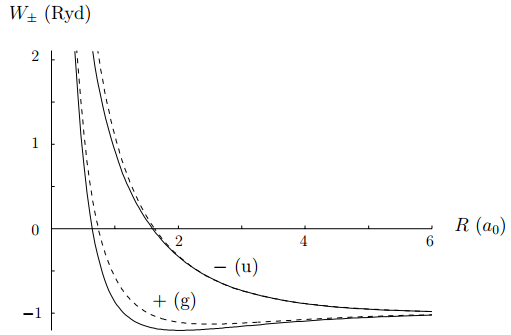
\includegraphics[scale=0.3]{img/image5.png}
	\captionof{figure}{Approximation $W_\pm$}
\end{wrapfigure}
Si les protons sont loin l'un de l'autre, l'électron a une forte probabilité de se trouver 
au voisinage de l'un d'entre eux pour former un atome d'hydrogène. La fonctions d'essai
doit refléter le fait que l’électron a autant de chance de se trouver à l'un ou à l'autre.
Soit $\psi_{1s}$  la fonction d'onde de l'état fondamental d'un atome d'hydrogène $\psi_{1s}
(\vec{r}) = \pi^{-1/2}a_0^{-3/2}e^{-r/a_0}$. Nos fonctions d'essais (non normées) seront alors : 
\begin{equation}
	\left\{\begin{array}{ll}
		\phi_+(\vec{r}) &= \psi_{1s}(\vec{r}+\frac{1}{2}\vec{R})+\psi_{1s}(\vec{r}-\frac{1}{2}\vec{R})\\
		\phi_-(\vec{r}) &= \psi_{1s}(\vec{r}+\frac{1}{2}\vec{R})-\psi_{1s}(\vec{r}-\frac{1}{2}\vec{R})
	\end{array}\right.
\end{equation}
Pour chaque valeur de $R$, on peut calculer $W_\pm(R)$ qui majore exactement l'énergie de l'équation
approchée. La courbe $W_-$ décroit de façon monotone mais $W_+$ possède un minimum : $\phi_-$ est 
antiliante alors que $\phi_+$ est liante. Cette dernière suggère que la molécule existe : comme 
en plus le minimum est inférieur -1 Ryd (système dissocié), l'ion $H_2^+$ possède une position 
d'équilibre stable : $\phi_+$ est une \textit{orbitale liante}.\\
L'énergie de dissociation est l'énergie à fournir pour dissocier le système : 
\begin{equation}
	D(H_2^+) = [-1-E_0(H_2^+)]\ Ryd > 0
\end{equation}
Avec nos fonctions d'essais, on trouve $R_0\approx 2.5\ a_0 \rightarrow D(H_2^+) \approx 0.13\ 
Ryd$\footnote{Une étude plus rigoureuse donne $D(H_2^+) \approx 0.13\ Ryd \approx 2.7\ eV$.}\\

Les densités de probabilités montrent bien une zone de probabilité de présence nulle pour l'
orbitale $\phi_-$ : l'électron ne peut assurer la cohésion du système des deux protons, ce qui
n'est pas le cas pour $\phi_+$. On note souvent l'orbitale liante $1s\sigma_g$ et l'antiliante
$1s\sigma_u^*$, orbitales correspondant à $m=0$. Les valeurs de $m$ sont représentées par $\sigma\
(m=0), \pi\ (m=1),\dots$ comme $s,p,d,\dots$ mais pour $m$ ! 


\section{La molécule d'hydrogène $H_2$}
Les analyses sont identiques, si ce n'est que c'est un peu plus laborieux (les fonctions d'essais
doivent tenir compte du spin, parité, ...). Lire 150-154.


\section{Vibrations des molécules diatomiques}
Les noyaux ont jusqu'ici été considérés fixes, mais ils sont en réalités des objets quantiques 
pouvant vibrés. "Le mouvement des électrons étant plus rapide, on peut imaginer que l'énergie 
totale d'origine électronique est une énergie potentielle pour le mouvement des noyaux qui s'
ajoute à leur énergie de répulsion coulombienne : la différence de vitesses des deux types de 
particules permet à l'énergie électronique de varier lors d'un déplacement des noyaux pour s'
adapter à leurs nouvelles positions."\footnote{A éclaircir}\\

La vibration se fait suivant la ligne joignant les positions d'équilibres, mouvement décrit par :
\begin{equation}
	\left[-\frac{\hbar^2}{2\mu}\frac{d^2}{dR^2} +V_{vib}(R)-V_{vib}(R_0)\right]u(R) = E_{vib}u(R)
\end{equation}
où $\mu$ est la masse réduite des noyaux, $R_0$ le minimum du potentiel $V_{vib}$ et $E_{vib}$ l'
\textit{énergie de vibration}.\\
Si la fonction d'essai est liante, le potentiel possède un creux à une distance $R_0$ : en son 
voisinage, on peut utiliser l'\textit{approximation harmonique} :
\begin{equation}
	V_{vib}(R) \approx V_{vib}(R_0) + \frac{1}{2}V_{vib}''(R_0)(R-R_0)^2
\end{equation}
où le terme d'ordre 1 est nul par définition de $R_0 ; V'(R_0)=0$. Avec la définition $V_{vib}'' 
= \mu\omega^2$ et le changement de variable $x=R-R_0$ on retrouve l'équation de l'oscillateur 
harmonique à une dimension :
\begin{equation}
	E_{vib} \approx (n_v+\frac{1}{2})\hbar\omega
\end{equation}
où $n_v$ est le \textit{nombre quantique de vibration}. La remarque fin de page 156 est 
intéressante.

\section{Rotation des molécules diatomiques}
Comme ce n'est pas forcément sphérique, la rotation peu jouer. Par la règle de correspondance, 
l'hamiltonien de rotation dépend du moment cinétique orbital $\vec{L}$ :
\begin{equation}
	H_{rot} = \frac{L^2}{2\mathcal{I}}
\end{equation}
où $\mathcal{I} = \mu R_0^2$, le moment d'inertie (cf. \textit{Mécanique Rationnelle II}) des deux 
masses $m_A,m_B$ situées à $R_0$ l'un de l'autre.  Les valeurs propres sont les \textit{énergies de 
	rotation} :
\begin{equation}
	E_{rot,l} = \frac{\hbar^2}{2\mathcal{I}}l(l+1)
\end{equation}
où ici $l$ est le \textit{nombre quantique de rotation}. En étudiant les différents types d'énergies, 
on remarque que :
\begin{equation}
	E_{rot} < E_{vib} < E_e
\end{equation}
Sur chaque niveau électronique apparaît un spectre de vibration composé de niveau distant de $\hbar
\omega$ et chaque niveau de vibration porte un spectre de vibration où l'écart est donné par 
$\frac{\hbar^2}{\mathcal{I}}(l+1)$.












\chapter{Les noyaux}
\section{La physique nucléaire}
Les dimensions nucléaires sont $10^5$ fois plus petites que les dimensions atomiques, mais les 
énergies y sont $10^5$ fois plus grandes ! Ces différences justifie le fait de négliger la 
présence d'électrons lors de l'étude du noyau.

\section{Neutrons et protons}
Les deux particules ont de peu la même masse : $m_p \approx 1836.15\ m_e, m_n = 1838.68\ m_e$. Le
rapport de leurs masses est proche de l'unité $\frac{m_n}{m_p}\approx1.00138$.\\
Le fait que la masse du neutron soit plus élevée rend ce dernier instable : son énergie de masse 
est suffisante pour une désintégration $\beta$.\\

Le neutron, particule neutre, possède un moment magnétique non nul : il est constitué de particules
chargées. Ce-dernier est constitué de \textit{quarks} de charge fractionnaire $\pm 2e/3$, jamais 
observé isolément. Sauf en haute énergie, on négligera sa structure interne (bonne approximation).

\section{Stabilité des noyaux}
Les noyaux possèdent $Z$ protons et $N$ neutrons ; le nombre de masse $A = N + Z$. Un peu de 
woordenschat! Le système composé d'un proton et d'un neutron est un \textit{deuton}. Deux atomes ayant le même 
$A$ sont des \textit{isobares}. Deux atomes ayant le même $Z$ sont des \textit{isotopes} (même 
propriétés chimiques).\\
Un noyau n'est stable que si son énergie $E$ est inférieure à toute les énergies des différents 
seuils de dissociation : 

\begin{equation}
	E < \max\ E_{seuil}
	\label{eq:seuil}
\end{equation}
Le neutron isolé est instable, mais stable dans le deuton : la stabilité est liée à l'énergie 
totale d'un système mais \textbf{pas} à la stabilité de ses composants isolés. \\
Certains noyaux sont stables mais ne vérifient pas \autoref{eq:seuil} car il faut tenir compte 
de la \textit{durée moyenne pour avoir dissociation} $\tau$. Un noyau est stable si $\tau >$ à
l'age de l'univers $\approx 5\times10^{17}\ s$.


\section{Énergie de liaison}
L'\textit{énergie de liaison} est la différence entre la somme des énergies de masses des neutrons 
et protons qui constituent le noyau et l'énergie de masse de ce noyau : 
\begin{equation}
	B = (Nm_n + Zm_p - M)c^2
\end{equation}
Le noyau est stable si $B>0$. On remarque que $B \approx\propto A$ pour $A>10$ :
\begin{equation}
	\frac{B}{A} \approx 8 \pm 1\ MeV
	\label{eq:stauration}
\end{equation}
La propriété \autoref{eq:stauration} est la \textit{saturation}. $B$ et $A$ sont liés à cause de la 
portée des forces nucléaires: un nucléon n’interagit qu'avec un nombre limité de ses voisins, l'
énergie de liaison dépend alors peu de la taille du noyau. Deux cas sont cool :
\begin{enumerate}
	\item Un noyau lourd est brisé $\rightarrow$ les fragments ont une charge plus petite $\rightarrow$ ils
	sont mieux liés que lui
	\item Un noyau léger est fusionné $\rightarrow$ le noyau résultant a une charge plus grande$\rightarrow$
	il est mieux lié que lui
\end{enumerate}
$\Rightarrow$ La variation d'énergie de liaison libère de l'énergie (sous forme d'énergie cinétique).


\section{Rayon et densité nucléaire}
Les nucléons n'interagissent fortement qu'avec leurs proches voisins\footnote{Faible portée de l'
	interaction forte} : $V \propto A$. Si le noyau est sphérique, son rayon est proportionnel à $A^{
	1/3}$ :
\begin{equation}
	r = r_0A^{1/3}\ \ \text{avec }\ r_0 \approx 1.2\ fm
\end{equation}
Comme la masse $\propto$ nombre de nucléons et au volume, la masse volumique est pratiquement indépendante
de $A$ : la densité nucléaire vaut : 
\begin{equation}
	\rho = \frac{A}{\frac{4\pi}{3}r_0^3A}\approx 0.14\ \text{nucléons/fm$^3$} = 1.4\times
	10^{44}\ \text{nucléons/m$^3$}
\end{equation}

\section{Radioactivité $\alpha$}
Certains noyaux lors de l'émission d'un noyau $^4He$ (particule $\alpha$) ne sont pas stables. Il 
y a probabilité de formation d'une particule $\alpha$ à partir  de $2 p^+$ et $2 e^-$\footnote{A la 
	surface du noyau car moins de répulsion}, mais pour être émise il faut passer par l'effet tunnel : 
tant que les 4 nucléons sont toujours dans le noyau, l'\textit{attraction} nucléaire forte supplante 
la \textit{répulsion} coulombienne. La différence de signe et de portée créent une barrière de 
potentiel que la particule doit franchir. En son sommet, les forces attractives et répulsives se 
neutralisent : l'émission de la particule $\alpha$ est conditionnée par la probabilité de passer outre
cette barrière par effet tunnel.

\section{Fission}
Les noyaux lourds ne vérifient pas \autoref{eq:seuil} lors d'une fission en deux fragments : $E_{
	seuil} < E$ car la répulsion coulombienne est plus faible lorsqu'elle est répartie en deux noyaux.
Mais ici aussi, une barrière de potentiel s'oppose à toute dissociation et leur durée de vie moyenne
est de perpet.\\

Cependant, on observe parfois la \textit{fission spontanée} : se dissocie seul après un certain temps
et balance de l'énergie cinétique avec les fragments : encore une fois, il y a une barrière de 
potentiel à passer et la probabilité de fission spontanée décroit exponentiellement lorsque la 
barrière s'élargit comme ..\ ....\ !\\
On peut également aider la fission en apportant de l'énergie au noyau par collision d'un neutron : 
\textit{fission induite}.


\section{Fusion}
En formant un noyau plus lourd, on augmente l'énergie de liaison, récupérée sous la forme d'énergie
cinétique. S'en suit une petite histoire sur l'avancée de cette technique, page 169.



















\part{Physique statistique}
\setcounter{chapter}{12}
\chapter{Principes de la physique statistique}
\section{Introduction}
Le but de la mécanique statistique est de décrire les propriétés de systèmes macroscopiques à partir des 
propriétés des systèmes microscopiques. Travailler avec deux ordres de grandeur si différents obligera 
l'utilisation simplificatrices.

\section{Idées fondamentales}
Quatre idées fondamentales sont à retenir sur la physique statistique
\begin{enumerate}
	\item Elle concerne des systèmes macro ayant un \textit{très grand nombre} de systèmes micro.
	\begin{itemize}
		\item Une idée de grandeur est le  nombre d'Avogadro $N_A \approx 6.022\times 10^{23}$. Comme ces
		nombres sont grands, on pourra facilement négliger un terme par rapport à eux.
	\end{itemize}
	\item Les \textit{équations de la physique quantique} décrivent les systèmes micro, mais celles-ci peuvent
	être simplifiées.
	\begin{itemize}
		\item Il faut tenir compte de l'indiscernabilité : le nombre de particules étant important, on trouvera
		forcément plusieurs fois les mêmes.
		\item Ce nombre étant immensément grand, tous les détails "micro" ne doivent pas forcément être pris 
		en compte\footnote{Parfois la physique classique suffit !}.
		\item Utiliser une équation de Schrödinger par particule n'est pas un traitement possible.
	\end{itemize}
	\item Les \textit{lois de conservations} sont respectées
	\begin{itemize}
		\item Comme l'énergie, la conservation du nombre de particules d'un certain type, ...
	\end{itemize}
	\item Les propriétés sont obtenues par des moyennes sur un \textit{ensemble statistique}.
	\begin{itemize}
		\item Il s'agit d'un ensemble fictif constitué d'un très grand nombre de systèmes identiques au 
		système étudié. 
		\item Ces moyennes sont basées sur les propriétés microscopiques.
	\end{itemize}
\end{enumerate}


\section{États d'un système macroscopique}
Nous allons nous intéresser ici uniquement aux systèmes macroscopiques : on ne connaîtra par exemple 
jamais la vitesse de chaque particule mais bien une \textit{vitesse moyenne}. Un peu de vocabulaire :
\begin{description}
	\item[Système isolé] ; Ne peut échanger ni énergie, ni particules avec son environnement : l'énergie 
	de ce système est fixe.
	\item[Système fermé] ; Ne peut pas échanger de particules mais peut échanger de l'énergie.
	\item[Variable d'état] ; Caractérise l'état macroscopique. Des relations existent entre elles et 
	porte le nom d'\textit{équation d'état}. Ces variables peuvent être \textit{intensives} (indépendante 
	du nombre de particules) ou \textit{extensives} (l'inverse hyhy).
	\item[Macroétat] ; Pour un système isolé, il est caractérisé par la donnée des grandeurs physiques 
	mesurables à l'échelle macro. C'est l'objet de la thermodynamique.
	\item[Microétat] ; Pour un système isolé, il est caractérisé par une fonction d'onde.
	\item[État accessible] ; État microscopique (microétat) qui est compatible avec les propriétés 
	macroscopiques. Seuls ces états doivent être pris en compte pour étudier les propriétés du système
	macroscopique considéré.
\end{description}


\section{Équilibre thermodynamique}
Un système isolé est à l'\textit{équilibre thermodynamique} si les propriétés macroscopiques de ce 
système ne dépendent pas du temps (macroétat indépendant du temps) : on se fiche de savoir comment le
système est arrivé à l'équilibre. Tout ceci ne veut par contre pas dire que ses propriétés micro ne 
varient pas, mais on n'en tient pas compte.

\section{Postulat fondamental de la physique statistique}
Comme la physique quantique, la physique statistique se base sur certains postulats. Le souci est 
que l'on ne peut pas considéré qu'un système soit dans un état accessible précis\footnote{Le système
	ne pouvait pas rester indéfiniment dans un état quantique exact.} mais l'on peut imaginer qu'il soit 
décrit par un \textit{mélange} de ces états accessibles :
\begin{center}
	\textsc{Postulat fondamental} :\\
	\textit{Les états accessibles d'un système isolé à l'équilibre sont équiprobables.}
\end{center}
Pour l'appliquer on considère un \textit{ensemble microcanonique}, c'est-à-dire un ensemble statistique
fictif constitué d'un grand nombre de copies identiques du système isolé, tous à même énergie mais se 
trouvant tous dans un état accessible différent.\\
Les propriétés du système macro seront les plus rencontrée dans cet ensemble, ce qui peut se
faire par un calcul des probabilités ou on considérant la \textit{moyenne} des propriétés des copies.
$\rightarrow$ Les propriétés observées sont celles qui ont le plus de chance de se produire.\\
Si les probabilités ne sont pas identiques, c'est que le système n'est pas à l'équilibre : il mettra le 
\textit{temps de relaxation} pour s'y ramener.


\section{Postulat de l'entropie}
La somme des énergies est une constante, mais la répartition peut se faire de plusieurs façon 
différentes. Supposons que l'énergie est comprise entre $E$ et $E+\delta E$, où $\delta$ est la
précision de l'appareil. Soit $\Omega(E)$ le nombre de microétats accessibles dont l'énergie est
entre $E$ et $E+\delta E$. Comme tous ces états sont équiprobables, on peut effectuer une moyenne
sur les propriétés de tous les états accessibles d'un ensemble microcanonique.\\

Selon la 2e loi de la thermodynamique, si le système n'est pas à l'équilibre il va  
maximiser son \textit{entropie}. \textit{Interprétation statistique} : le système va évoluer vers
un macroétat pour lequel les états accessibles ont tous la même probabilité.
\begin{center}
	\textsc{Postulat de l'entropie}\\
	\textit{L'entropie $S$ d'un système isolé à l'équilibre est proportionnelle au logarithme du nombre
		$\Omega$ d'état accessibles (où $k_B$ est la constante de Boltzmann) :}
	\begin{equation}
		S = k_B\ln\Omega
		\label{eq:entropie}
	\end{equation}
\end{center}
Ce postulat relie l'entropie du système à la probabilité qu'il soit dans un état accessible 
quelconque.\\
L'entropie $S$ est ainsi une grandeur \textit{extensive} : si le système est divisé en deux, le 
nombre d'état accessible du système complet est égal au nombres de paires d'états accessibles des
systèmes partiels :
\begin{equation}
	\Omega = \Omega_1\Omega_2
\end{equation}
Avec \autoref{eq:entropie} on retrouve bien $S = S_1+S_2$. La constante $k_B \approx 8.617\times
10^{-5} eV/K$ n'est pas une constante fondamentale mais juste le facteur de $\propto$ entre $S$
et $\ln\Omega$.\footnote{L'entropie n'est pas indépendante de $\delta E$ mais son apport est 
	faible et peut être négligé.}\\

La relation \autoref{eq:entropie} peut être inversée pour donner :
\begin{equation}
	\Omega = e^{S/k_B}
\end{equation}
Comme il s'agit d'une grandeur extensive, elle est proportionnelle au nombre $N$ de particules 
constituant le système :
\begin{equation}
	\Omega = e^{N(S^{(1)}/k_B)}
\end{equation}
où $S^{(1)}$ est l'entropie par particule.


\section{La température}
Le thermodynamique défini la \textit{température (absolue)} :
\begin{equation}
	\frac{1}{T} = \left(\dfrac{\partial S}{\partial U}\right)_{V,N}
\end{equation}
où $U$ est l'énergie interne du système. En utilisant \autoref{eq:entropie}, on obtient la \textit{
	définition statistique de l'entropie} :
\begin{equation}
	\frac{1}{k_BT} = \left(\dfrac{\partial \ln\Omega}{\partial U}\right)_{V,N}
	\label{eq:entropieStat}
\end{equation}
On voit que c'est $k_BT$ qui a un sens physique et pas l'un ou l'autre pris séparément. La 
définition \autoref{eq:entropieStat} est théorique si le système est isolé. Pour un système 
fermé, l'entropie peut alors varier avec l'énergie et la notion de température devient stylée.

\subsection*{Exemple : la thermalisation}
Soit deux systèmes $A$ et $B$ en \textit{contact thermique}. Le nombre d'état du système
$A$ (resp. $B$) est noté $\Omega_A(U_A)$ (resp. $\Omega_B(U_B)$) où $U_A$ (resp. $U_B$) est 
l'énergie interne du système $A$ (resp. $B$). Les énergies internent peuvent varier, mais 
pas l'énergie totale :
\begin{equation}
	U_T = U_A+U_B
\end{equation}
Le nombre d'état accessible est le produit des états accessibles de chaque système (
écrivons le comme fonction de $U_A$) :
\begin{equation}
	\Omega(U_A) = \Omega_A(U_A)\Omega_B(U_T-U_A)
\end{equation}
L'énergie $U_A$ la plus probable est celle qui correspond à la plus grande valeur de $
\Omega$. Maximisons :
\begin{equation}
	\left(\dfrac{\partial \ln\Omega}{\partial U_A}\right)_V,N =	\left(\dfrac{\partial \ln\Omega_A}
	{\partial U_A}\right)_V,N - 	\left(\dfrac{\partial \ln\Omega_B}{\partial U_B}\right)_V,N = 0
	\label{eq:MaxUA}
\end{equation}
Avec \autoref{eq:entropieStat}, \autoref{eq:MaxUA} s'écrit :
\begin{equation}
	\frac{1}{k_BT_A} = \frac{1}{k_BT_B}\ \ \ \ \Leftrightarrow\ \ \ T_A = T_B
\end{equation}
L'équilibre statistique correspond bien à l'égalité des températures comme vérifié
expérimentalement.


\section{La pression et le potentiel chimique}
L'entropie est également fonction de $V$, le volume du système. De façon analogue à la 
température, on définit la pression :
\begin{equation}
	P = T\left(\dfrac{\partial S}{\partial V}\right)_{U,N}
\end{equation}
et le potentiel chimique :
\begin{equation}
	\mu = -T\left(\dfrac{\partial S}{\partial N}\right)_{U,V}
\end{equation}
Ces deux grandeurs s'équilibrent aussi lors d'une thermalisation. Le potentiel semble être 
toujours négatif : c'est bien le cas en général mais on verra qu'il existe cependant des 
cas ou $\mu$ est positif.





\chapter{Système en équilibre avec un thermostat}
\section{Définition}
Soit un système fermé, marco ou micro, en contact avec un \textit{thermostat}, c'est-à-dire
un système dont la température ne change pas. Le système étudié ici est composé du système 
$S$, du thermostat $R$ et ici non plus, l'énergie totale ne varie pas (où $U_S \ll U_R$) :
\begin{equation}
	U_T = U_S + U_R
\end{equation}

\section{Distribution de probabilités de Boltzmann}
Le nombre total $\Omega_T$ de microétats accessibles est donné par :
\begin{equation}
	\Omega_T = \sum_{U_S+U_R=U_T} \Omega_S(U_S)\Omega_R(U_R)
	\label{eq:SomMic}
\end{equation}
Cette somme porte sur toutes les façon de distribuer l'énergie entre $S$ et $R$. Intéressons-
nous à  un des termes de \autoref{eq:SomMic} pour une énergie $U_S$ du système $S$. Le nombre
d'état accessible est alors :
\begin{equation}
	\Omega(U_S) = \Omega_S(U_S)\Omega_R(U_T-U_S)
\end{equation}
Choisissons pour $U_S$ l'énergie $E_i$ correspondant à la fonction d'onde $\psi_i$ : on a un
état et donc $\Omega_S(E_i) = 1$ pour obtenir\footnote{Le $\Omega(E_i)$ renseigne simplement 
	que le nombre d'état total $\Omega$ est fonction de $E_i$ (et $U_T$ est une constante).} :
\begin{equation}
	\Omega(E_i) = \Omega_R(U_T-E_i)
	\label{eq:aLog}
\end{equation}
avec $E_i \ll U_T$. Le nombre total de microétat : 
\begin{equation}
	\Omega_T = \sum_j \Omega(E_j)
\end{equation}
En prenant le logarithme de \autoref{eq:aLog} et en développant au premier ordre (comme $E_i
\ll U_T$) :
\begin{equation}
	\ln\Omega(E_i) \approx \ln\Omega_R(U_T) - E_i\left[\dfrac{\partial \ln\Omega_R}{\partial U_R}
	\right]_{U_T}
	\label{eq:DerivPart}
\end{equation}
On peut considérer que la dérivée partielle de \autoref{eq:DerivPart} est constante et en 
utilisant \autoref{eq:entropieStat}, le nombre total d'états accessibles à l'énergie $E_i$ 
devient :
\begin{equation}
	\Omega(E_i) = Ce^{-E_i/k_BT}
\end{equation}
où $C = \Omega_R(U_R)$.\newpage

Appliquons le postulat fondamental. La probabilité $p_i$ que le système global comporte 
un système $S$ dans un état d'énergie $E_i$ est donné par le produit des cas favorable
($\Omega(E_i)$) sur le nombre de cas total $\Omega_T$ :
\begin{equation}
	p_i = \dfrac{\Omega(E_i)}{\sum_j\Omega(E_j)}
\end{equation}
Ces probabilités correspondent à la \textit{distribution des probabilités de Boltzmann} :
\begin{equation}
	p_i =  \dfrac{e^{-E_i/k_BT}}{\sum_j e^{-E_j/k_BT}}
	\label{eq:DistriBoltz}
\end{equation}
La seule donnée restant du thermostat est sa température $T$. En posant 
\begin{equation}
	Z = \sum_j e^{-E_j/k_BT}
	\label{eq:fctPartCan}
\end{equation}
nommée \textit{fonction de partition canonique}, l'équation \autoref{eq:DistriBoltz} 
devient:
\begin{equation}
	p_i = \frac{1}{Z}e^{-E_j/k_BT}
	\label{eq:probaBoltz}
\end{equation}
Ces probabilités permettent de définir l'énergie interne comme étant l'énergie moyenne:
\begin{equation}
	U = \sum_i p_iE_i = \dfrac{\sum_i E_ie^{-E_i/k_BT}}{\sum_ie^{-E_i/k_BT}}
	\label{eq:U}
\end{equation}
qui montre que la température est reliée à l'énergie interne par une fonction dépendant de 
tous les microétats. \textit{Interprétation :} la température $T$ est un paramètre qui fixe
l'énergie moyenne du système en contact avec le thermostat.\\
L'équation \autoref{eq:U} permet d'interpréter les notions de chaleur et travail. Une 
variation de $U$ s'écrit (en restant dans l'équilibre) :
\begin{equation}
	\delta U = \sum_i E_i\delta p_i + \sum_i p_i\delta E_i
\end{equation}
En mettant cette expression en parallèle avec 
\begin{equation}
	\delta U = \delta Q + \delta W
\end{equation}
On peut procéder à une identification terme à terme (interprétation page 196).



\section{Entropie canonique}
Considérons un système constitué d'un grand nombre $M-1$ répliques identiques et 
indiscernable du système $S$ en contact de façon à avoir des échanges thermiques, mais dont
le système total est isolé : il s'agit d'un \textit{ensemble canonique}.\\
Les état accessibles (dont le nombre est noté $\Omega_S$) de ces systèmes sont les fonctions 
d'ondes $\psi_i$ peuplés par la distribution de Boltzmann. Soit $m_i$, le nombre de répliques
qui sont dans un état de fonction d'onde $\psi_i$ :
\begin{equation}
	m_i = p_i M = \dfrac{e^{-E_i/k_BT}}{\sum_{j=1}^{\Omega_S} e^{-E_j/k_BT}}M
	\label{eq:DefMi}
\end{equation}
où $M = \sum_{i=1}^{\Omega_S} m_i$. Les répliques de $S$ sont indiscernables : le nombre de 
façon que $m_1$ d'entre elles soient $\psi_1$, $m_2$ soient $\psi_2,\dots$ est donné par 
la combinaison :
\begin{equation}
	\Omega(m_1,m_2,\dots) = \frac{M!}{m_1!m_2!\dots}
	\label{eq:OmegaTot}
\end{equation}
Comme l'ensemble est isolé, l'entropie \textit{totale} est donnée par (ou $\Omega$ est donné
par \autoref{eq:OmegaTot}) :
\begin{equation}
	S_M = k_B\ln\Omega
\end{equation}
Avec l'approximation des grands nombres :
\begin{equation}
	S_M = k_B\left(M\ln M - \sum_{i=1}^{\Omega_S} m_i\ln m_i\right) = -k_B\sum_{i=1}^{\Omega_S} m_i
	\ln m_i
\end{equation}
L'entropie moyenne est donné par $S = S_M/M$ :
\begin{equation}
	S = -k_B\sum_{i=1}^{\Omega_S} \frac{m_i}{M}\ln\frac{m_i}{M}
\end{equation}
D'après \autoref{eq:DefMi} :
\begin{equation}
	S = -k_B\sum_{i=1}^{\Omega_S} p_i\ln p_i
\end{equation}
Ce qui est l'expression de l'entropie d'un système à température donnée. Celle-ci est aussi
valable hors équilibre. La page 198 montre comment notre dernière expression peut devenir 
\begin{equation}
	S = \frac{U}{T} + k_B\ln Z
	\label{eq:AutreRel}
\end{equation}

\section{Fonction de partition et énergie libre}
L'énergie libre 
\begin{equation}
	F = U -TS
\end{equation}
combinée avec \autoref{eq:AutreRel} permet d'obtenir une importante relation liant l'énergie
libre et la fonction de partition :
\begin{equation}
	F = -k_BT\ln Z
\end{equation}
La fonction de partition se calcule à partir des propriétés micro alors que l'énergie libre 
détermine les propriétés macro. Pour plus de calcul cool, se référer à la page 199.








\chapter{Propriétés des gaz}
\section{Types de gaz}
On suppose que le gaz est composé d'une seule sorte de particules/molécules. Les propriétés d'un gaz 
dépendent des propriétés des particules qui le composent et surtout leurs énergies d'excitations.
Les collisions entre molécules (qui possèdes des niveaux excités à des énergies bien plus faibles
que les gaz rares) excitent les molécules et modifie les propriétés thermodynamiques du gaz.


\section{Gaz parfait de particules discernables}
Un gaz est dit \textit{parfait} lorsqu'on peut négliger les interactions entre particules et que 
l'énergie interne est constante. Pour décrire un tel gaz, considérons une boite de coté $a$. 
On fera l'hypothèse (peu réaliste) que chaque particule est discernable : on calcule pour une 
et après on multiplie le tout.\\
Les énergies d'une particule dans une boite et les fonctions d'ondes correspondantes sont données 
par :
\begin{equation}
	E_n = \frac{n^2\pi^2\hbar^2}{2ma^2},\ \ \ \ \ \ \ \ \  \psi_n(x) = \sqrt{\dfrac{2}{a}}\sin
	\dfrac{n\pi x}{a}
\end{equation}

Le résultat est facilement généralisable en 3D :
\begin{equation}
	\begin{array}{ll}
		E(n_x,n_y,n_z)          & = (n_x^2 +n_y^2+n_z^2)\frac{\pi^2\hbar^2}{2ma^2}                                        \\
		\psi_{n_xn_yn_z}(x,y,z) & = (\frac{2}{a})^(3/2)\sin\frac{n_x\pi x}{a}\sin\frac{n_y\pi y}{a}\sin\frac{n_z\pi z}{a} 
	\end{array} 
\end{equation}
Ceci va permettre le calcul des propriétés thermodynamiques d'une seule particule à l'équilibre avec
le thermostat constitué des autres particules. En introduisant le paramètre sans dimension :
\begin{equation}
	\gamma = \dfrac{\pi^2\hbar^2}{2ma^2k_BT}
\end{equation} 
la fonction de partition du système s'écrit (le $(1)$ rappelle que le système ne possède qu'une
seule particule) :
\begin{equation}
	Z^{(1)} = \sum_{n_x=1}^\infty\sum_{n_y=1}^\infty\sum_{n_z=1}^\infty e^{-\gamma(n_x^2 +n_y^2+n_z^2)}
	= \left(\sum_{n=1}^\infty e^{-\gamma n^2}\right)^3
\end{equation}
En utilisant l'approximation\footnote{Si on divise le domaine d'intégration en intervalles unitaires et
	que l'on remplace dans chaque intervalle la fonction par son majorant, on retrouve bien la série.} :
\begin{equation}
	\sum_{n=1}^\infty e^{-\gamma n^2} \approx \int_0^\infty e^{-\gamma u^2}du = \dfrac{1}{2}\sqrt{\dfrac{\pi}
		{\gamma}}
	\label{eq:ApproxSerie}
\end{equation}
Cette approximation est d'autant meilleure que l’intégrande varie peu sur chaque intervalle unitaire :
possible si $\gamma \ll 1$ ce qui est le cas ici. Cette hypothèse revient à négliger la quantification;
il s'agit d'une \textit{approximation classique}. On a alors, pour un volume $V=a^3$ :
\begin{equation}
	Z^{(1)} \approx \dfrac{1}{8}\left(\dfrac{\pi}{\gamma}\right)^{3/2} = \left(\dfrac{mk_BT}{2\pi\hbar^2}
	\right)^{3/2}V
	\label{eq:z1}
\end{equation}
L'équation (14.35) du syllabus (sorry pfpfpf) permet de déduire la pression due à une seule particule:
\begin{equation}
	P^{(1)} = \dfrac{k_BT}{V}
\end{equation}
Dans un système à  $N_A$ particules constituant une mole de gaz, la pression totale $P = N_AP^{(1)}$ la
\textit{loi de gaz parfaits}:
\begin{equation}
	PV = RT
\end{equation}
où la \textit{constante des gaz parfaits} $R = N_Ak_B \approx 8.314\ \text{J mole$^{-1}$ K$^{-1}$}$.\\
L'entropie est donnée par (toujours dans le syllabus, section 14.4\footnote{A faire}) (14.37) :
\begin{equation}
	S^{(1)} = k_B(\frac{3}{2}+\ln Z^{(1)}) = \frac{3}{2}k_B\left[1+\ln\left(\dfrac{mk_BT}{2\pi\hbar^2}V^{
		2/3}\right)\right]
\end{equation}
et l'équation (14.37) permet de calculer la capacité calorifique à volume constant 
\begin{equation}
	C_V^{(1)} = T\left(\frac{\partial S^{(1)}}{\partial T}\right)_V = \frac{3}{2}k_B
\end{equation}
et donc la \textit{chaleur spécifique molaire}
\begin{equation}
	c_V = N_AC_V^ {(1)} = \frac{3}{2}R
\end{equation}



\section{Distribution de Maxwell des vitesses}
Que peut on maintenant dire au niveau micro? Les vitesses des particules sont distribuées suivant
une loi simple trouvée par Maxwell. On considérera ici un gaz parfait et on fera l'approximation
classique.\\
Il faut exprimer les probabilités en fonction de la vitesse $\vec{v}$ à partir de $E = \frac{1}{2}
mv^2$. A partir de \autoref{eq:probaBoltz}, on obtient :
\begin{equation}
	p(\vec{v}) = Z^{-1}e^{-mv^2/2k_BT}
\end{equation}
C'est la densité de probabilité pour qu'une particule ai une vitesse dont les composantes sont 
comprises entre $\vec{v}$ et $\vec{v} +d\vec{v}$.\\
La fonction de partition
\begin{equation}
	Z = \sum e^{-mv^2/2k_BT}
\end{equation}
doit elle être comprise comme une somme sur toutes les vitesses possibles :
\begin{equation}
	Z = \int_{-\infty}^\infty dv_x \int_{-\infty}^\infty dv_y \int_{-\infty}^\infty dv_z 
	e^{-mv^2/2k_BT}
\end{equation}
Avec \autoref{eq:ApproxSerie} on trouve
\begin{equation}
	Z = \left(\dfrac{2\pi k_BT}{m}\right)^{3/2}
\end{equation}
Comme la distribution de vitesses $p(\vec{v})$ ne dépend pas de l'orientation (normal que la 
distribution soit isotrope à l'équilibre). On peut remplacer cette distribution $p(\vec{v})$ 
par une distribution des valeurs de la vitesse indépendante de la direction en introduisant
les coordonnées sphériques\footnote{Pq ?}.\\
L'élément de volume devient : $dv_xdv_ydv_z = v^2dv\sin\theta_vd\theta_vd\phi_v$ pour finalement
trouver :
\begin{equation}
	F(v) = 4\pi\left(\dfrac{m}{2\pi k_BT}\right)^{3/2} v^2 e^{-mv^2/2k_BT}
\end{equation}
Il s'agit de la \textit{distribution de Maxwell des vitesses}. Elle possède en maximum en la 
vitesse (qui n'est \textbf{pas} la vitesse maximum!) : 
\begin{equation}
	v_{max} = \sqrt{\dfrac{2k_BT}{m}}
\end{equation}
Cette vitesse est la vitesse la plus probable. On peut utiliser cette distribution pour calculer 
la vitesse moyenne des particules dans le gaz :
\begin{equation}
	v_{moy} = \frac{2}{\sqrt{\pi}}v_{max} \approx 1.13 v_{max}
\end{equation}
On peut aussi calculer la vitesse en moyenne quadratique :
\begin{equation}
	\sqrt{\frac{3}{2}}v_{max} \approx 1.22 v_{max}
\end{equation}
Ce dernier résultat permet de calculer l'énergie cinétique moyenne des particules de gaz :
\begin{equation}
	E_{moy} = \frac{1}{2}mv^2_{quad} = \frac{3}{2}k_BT
\end{equation}

\section{Propriétés thermodynamiques des gaz dues aux rotations des molécules diatomiques}
On ne s'intéressait qu'à l'énergie cinétique mais il existe aussi des niveaux d'excitation 
interne dont l'énergie d'excitation est faible comme c'est le cas pour le mouvement de 
rotation. L'énergie de rotation étant $E_{rot} = \frac{\hbar^2}{2\mathcal{I}}l(l+1)$. Avec
\autoref{eq:fctPartCan} la fonction de partition s'écrit\footnote{Et avec son équivalent 
	utilisant la dégénérescence} :
\begin{equation}
	Z_{rot} = \sum_{l=0}^\infty\sum_{m=-l}^l e^{-\hbar^2l(l+1)/2\mathcal{I}k_BT} = \sum_{
		l=0}^\infty (2l+1)e^{-\hbar^2l(l+1)/2\mathcal{I}k_BT}
\end{equation}
Chaque fonction d'onde est caractérisée par $m$ et chaque niveau est dégénéré $g_l = 2l
+1$ fois. La grandeur
\begin{equation}
	\theta_r = \frac{\hbar^2}{2\mathcal{I}k_B}
\end{equation}
a les dimension d'une température : c'est la \textit{température caractéristique de 
	rotation}. La fonction de partition devient 
\begin{equation}
	Z_{rot} = \sum_{l=0}^\infty (2l+1)e^{-l(l+1)\theta_r/T}
	\label{eq:zrot}
\end{equation}
On peut alors appliquer les formules vues en section 14.4 pour trouver la capacité 
calorifique :
\begin{equation}
	C_{V,rot} = k_BT\left(\dfrac{\partial^2[T\ln Z_{rot}]}{\partial T^2}\right)_V
\end{equation}
A basse température ($T \ll \theta_r$) on peut obtenir en développant les deux premiers
termes pour ne pas avoir qu'une constante :
\begin{equation}
	\ln Z_{rot} \approx \ln(1+3e^{-2\theta_r/T}) \approx 3e^{-2\theta_r/T}
\end{equation}
La capacité calorifique par molécule vaut dès lors
\begin{equation}
	C_{V,rot} \approx 12 k_B \frac{\theta_r^2}{T^2}e^{-2\theta_r/T}
\end{equation}
A haute température ($\theta_r \ll T$), en remplaçant la série de \autoref{eq:zrot} par 
une intégrale comme fait précédemment, après changement de variable on obtient
\begin{equation}
	Z_{rot} \approx \frac{T}{\theta_r}
\end{equation}
Et on en tire
\begin{equation}
	C_{V,rot} \approx k_B
\end{equation}

\section{Propriétés thermodynamiques des gaz dues aux vibrations des molécules 
	diatomiques}
L'idée est toujours la même mais on fourni un peu plus d'énergie pour exciter cette fois
les niveaux de vibrations. L'énergie de vibration est donné par : $E_{vib} \approx (n_v
+\frac{1}{2} )\hbar\omega$. La fonction de partition :
\begin{equation}
	Z_{vib} = \sum_{n_v=0}^\infty e^{-(n_v+\frac{1}{2})\hbar\omega/k_BT} = \sum_{n_v=0}^\infty
	e^{-(n_v+\frac{1}{2})\theta_v/T}
\end{equation}
où $\theta_v = \hbar\omega/k_B$ est la \textit{température caractéristique de vibration}.
Pour $|x|<1$, on retrouve la série géométrique $(1-x)^{-1} = \sum_{n=0}^\infty x^n$. La 
série peut alors être sommée : 
\begin{equation}
	Z_{vib} = e^{-\theta_v/2T}\frac{1}{1-e^{-\theta_v/T}}
\end{equation}
Comme précédemment, on déduit la capacité calorifique :
\begin{equation}
	C_{V,vib} = k_B \frac{\theta_v^2}{T^2}\frac{e^{\theta_v/T}}{(e^{\theta_v/T}-1)^2}
\end{equation}
Lorsque $T$ est petit\footnote{C'est comme avant, non-détaillé ici.} :
\begin{equation}
	C_{V,vib} \approx k_B \frac{\theta_v^2}{T^2}e^{-\theta_v/T}
\end{equation}
Lorsque $T$ est grand :
\begin{equation}
	C_{V,vib} \approx k_B
\end{equation}


\section{Gaz de molécules diatomiques}
\begin{wrapfigure}[14]{r}{6cm}
	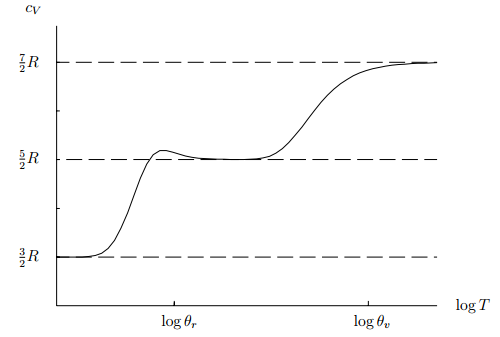
\includegraphics[scale=0.4]{img/image6.png}
	\captionof{figure}{Evolution de $c_V$ en fonction de $T$}
	\label{fig:cV}
\end{wrapfigure}
On prend maintenant compte de tout en même temps ! L'énergie totale est alors :
\begin{equation}
	E = E_{trans}(n_x,n_y,n_z) + E_{rot}(l) + E_{vib}(n_v)
\end{equation}
Avec l'expression de la fonction de partition, on arrive à la conclusion que :
\begin{equation}
	C_V = C_{V,trans} + C_{V,rot} + C_{V,vib}
\end{equation}
On se trouve initialement à l'état de translation avec une énergie $c_V = \frac{3}{2}R$.
Lorsqu'on donne une certaine énergie (sous forme de chaleur) on va pouvoir augmenter 
au maximum $c_V$ de $R$ pour avoir $\frac{5}{2}R$ (une augmentation de $k_B$ correspond à
une augmentation de $R$ au niveau mole) grâce à l'énergie de rotation ! Puis, avec l'énergie
de vibration on pourra encore augmenter de $R$ pour obtenir la valeur totale de $c_V = \frac{7}{2}
R$ comme on peut le voir à la \autoref{fig:cV}.

\section{Propriété des systèmes dont l'énergie est une somme de termes indépendants}
On peut généraliser tout ce qui a été obtenu précédemment à un nombre $n$ d'énergie.










\chapter{Mécanique statistique de particules identiques}
\section{Le paradoxe de Gibbs}
Jusqu'ici nous avons considéré les particules comme étant discernables. Cependant, comme 
nous allons le voir, cette hypothèse induit parfois en erreur. Considérons l'entropie d'une
particule de gaz et multiplions par $N$ pour le nombre de particules dans un volume $V$ :
\begin{equation}
	\tilde{S}(N,V) = \frac{3}{2}Nk_B\left[1+\ln\left(\dfrac{mk_BT}{2\pi\hbar^2}V^{2/3}\right)\right]
	\label{eq:FausseEntropie}
\end{equation}
Cette expression n'est pas correcte car l'entropie n'est pas extensive $S(\lambda N,\lambda V) != \lambda S(N,V)$.\\
On peut retrouver \autoref{eq:FausseEntropie} en partant de l'hamiltonien du système : 
$H = \sum_{i=1}^N \frac{p_i^2}{2m}$. L'énergie totale est la somme des énergies des $N$ particules
($E = E_1 + E_2 + \dots$) conduisant à la fonction de partition :
\begin{equation}
	\tilde{Z} = (Z^{(1)})^N
\end{equation}
où $Z^{(1)}$ est donné par \label{eq:z1}. En utilisant 
\begin{equation}
	S = k_B\left(\dfrac{\partial [T\ln Z]}{\partial T}\right)_{V,N}
	\label{eq:EntroCh15}
\end{equation}
on retrouve \autoref{eq:FausseEntropie} : c'est le paradoxe de Gibbs. Ce dernier à tout  de 
même réussi à le corriger empiriquement en partant de
\begin{equation}
	Z = \dfrac{(Z^{(1)^N})}{N!}
\end{equation}
où le dénominateur est le \textit{facteur de correction de Gibbs.} En utilisant \autoref{eq:EntroCh15}:
\begin{equation}
	\ln\ Z = N\ln\ Z^{(1)} - N\ln\ N + N
\end{equation}
on peut déduire l'expression correcte de l'entropie :
\begin{equation}
	S(N,V) = Nk_B\left\{\dfrac{5}{2}+\dfrac{3}{2}\ln\left[\dfrac{mk_BT}{2\pi\hbar^2}\left(\dfrac{V}{N}
	\right)^{2/3}\right]\right\}
\end{equation}
Cette fois-ci, grâce au rapport $V/N$, $S$ est bien extensive.

\section{Bosons et fermions sans interaction}
Il y a deux catégories au niveau de l'indiscernabilité : les bosons (spin entier) identiques décrits par 
une fonction d'onde symétrique et les fermions identiques par une fonction d'onde antisymétrique (spin 
demi-entier). Les atomes/molécules ne sont composés que de fermions ($e^-,p^+,n^0$). Le moment cinétique
total de deux particules de spin $1/2$ est entier et devient demi-entier lors de l'ajout d'un fermion :
\begin{center}
	\textit{Un atome, une molécule ou un noyau atomique est un boson si le nombre total d'électron, protons 
		et neutrons qui le composent est pair ou un fermion si ce nombre est impair.}
\end{center}
Considérons \textbf{deux fermions identiques} sans interactions. Une fonction d'onde antisymétrique de
ce système peut s'écrire grâce à Slater :
\begin{equation}
	\Psi_A(1,2) = \frac{1}{\sqrt{2}}\left|\begin{array}{cc}
		\psi_\alpha(1) & \psi_\alpha(2)\\
		\psi_\beta(1) & \psi_\beta(2)
	\end{array}\right|
\end{equation}
La valeur propre vaut $E = E_\alpha + E_\beta$ (où $E_\alpha \neq E_\beta$ si elles ne sont pas dégénérés) 
et $\Psi_A$ n'existe que si $\phi_\alpha\neq\phi_\beta$ à cause de Pauli (deux fermions identiques doivent 
être dans des états différents).\\
Considérons \textbf{deux bosons identiques} sans interactions. Une fonction d'onde symétrique :
\begin{equation}
	\Psi_S(1,2) = \left\{\begin{array}{ll}
		\psi_\alpha(1)\psi_\alpha(2), & (\alpha=\beta)\\
		\frac{1}{\sqrt{2}}[\psi_\alpha(1)\psi_\beta(2) + \psi_\beta(1)\psi_\alpha(2)], & (\alpha\neq\beta)
	\end{array}\right.
\end{equation}
Ici, rien n'empêche que $\alpha = \beta$. Pour les fermions, on peut généraliser ce résultat à $N$ fermions 
identiques :
\begin{equation}
	E = \sum_{\lambda=0}^{N-1} E_\lambda
\end{equation}
où toutes les énergies $E_\lambda$ doivent être différentes. Pour les bosons, ils peuvent eux se trouver
à plusieurs dans le même état avec une même fonction d'onde individuelle $\psi_\alpha$ :
\begin{equation}
	E = NE_0
\end{equation}

\section{Interprétation de la correction de Gibbs}
Soit un système de deux particules de même masse supposé \textit{discernable} où $E_\alpha$ et $E_\beta$ 
correspondent aux deux valeurs propres distinctes de $H(1)$ et $H(2)$ de fonction propre $\psi_\alpha$ et
$\psi_\beta$. Deux fonctions propres différentes de $H$\footnote{$H = H(1)+H(2)$.} sont données par :
\begin{equation}
	\begin{array}{ll}
		\Psi_{\alpha\beta}(1,2) & =  \psi_\alpha(1)\psi_\beta(2) \\
		\Psi_{\beta\alpha}(1,2) & =  \psi_\beta(1)\psi_\alpha(2) 
	\end{array}
\end{equation}
Elles correspondent cependant à la même énergie $E = E_\alpha+E_\beta$ ; lors du calcul de $Z$, l'énergie
$E$ est comptée deux fois ! Le facteur de correction de Gibbs permet d'éviter de compter plusieurs fois le
même étant individuel. Ceci reste une approximation, car on néglige la différence fermion/boson.



\section{Statistique de photons}
Soit un gaz de photons (boson) à température $T$. Leur nombre peut varier par absorption et émission avec
la paroi par exemple. Ils peuvent exister dans différents états d'énergie $\epsilon_1,\epsilon_2,\dots$ 
pouvant être relié à $\nu_\gamma$ ou $\lambda_\gamma$. Chacune des $\nu/\lambda$ caractérise un 
\textit{mode} $\gamma$ du champ EM. Le nombre de photons dans chaque niveau est noté $n_1,n_2,\dots$\footnote{
	On ne fait que \textit{compter} les photons, on les traite bien comme \textit{indiscernable}.} La 
fonction de partition est alors une somme sur tous ces nombres possibles :
\begin{equation}
	Z = \sum_{n_1,n_2,\dots} e^{-(n_1\epsilon_1 + n_2\epsilon_2 + \dots)/k_BT}
\end{equation}
On peut séparer les sommations, elle sont indépendantes. On va maintenant considérer chaque mode 
séparément et on mettra tout ensemble dans la prochaine section. Pour un mode donné, la fonction de 
partition vaut :
\begin{equation}
	\begin{array}{ll}
		Z_\gamma & = \sum_{n_\gamma=0}^\infty \left(e^{-\epsilon_\gamma/k_BT}\right)^{n_\gamma} \\
		& = \dfrac{1}{1-e^{-\epsilon_\gamma/k_BT}}                                     
	\end{array}
\end{equation}
D'après la distribution de Boltzman, la probabilité d'avoir $n_\gamma$ photons dans le niveau
$\epsilon_\gamma$ est :
\begin{equation}
	p(n_\gamma) = \dfrac{e^{-n_\gamma\epsilon_\gamma/k_BT}}{Z_\gamma}
\end{equation}
Le nombre moyen de photon d'énergie $\epsilon_\gamma$ est donné par la moyenne des $n_\gamma$ 
pondérés par les probabilités correspondantes :
\begin{equation}
	<n_\gamma> = \sum_{n_\gamma = 0}^\infty p(n_\gamma)n_\gamma = -k_BT\dfrac{\partial}{\partial\epsilon_
		\gamma}\ln Z_\gamma = \dfrac{1}{e^{\epsilon_\gamma/k_BT}-1}
\end{equation}
On considère en général l'énergie de ces modes comme continue : $\epsilon$ pour écrire l'expression du
nombre moyen de photon en fonction de l'énergie $\epsilon$ de ces photons, à température $T$ :
\begin{equation}
	n(\epsilon,T) = \dfrac{1}{e^{\epsilon/k_BT}-1}
\end{equation}
ce qui n'est rien d'autre que la \textit{distribution de Planck}. On observe que le nombre moyen de 
photons d'énergie données augmente avec la température. A  haute énergie :
\begin{equation}
	n(\epsilon,T) \approx e^{-\epsilon/k_BT} \ll 1,\ \ \ \ \ \ \ \ \ \ \ \ \ \ \ \ \ \ \ \  k_BT\ll\epsilon
\end{equation}
A basse énergie :
\begin{equation}
	n(\epsilon,T) \approx \frac{k_BT}{\epsilon} \gg 1,\ \ \ \ \ \ \ \ \ \ \ \ \ \ \ \ \ \ \ \ \epsilon\ll k_BT
\end{equation}
L'énergie moyenne du champ dans un mode donné vaut simplement le nombre moyen de photons fois l'énergie 
de ceux-ci :
\begin{equation}
	\overline{E}_\nu(T) = \dfrac{\epsilon_\nu}{e^{\epsilon_\nu/k_BT}-1} = \dfrac{h\nu}{e^{h\nu/k_BT}-1}
	\label{eq:ResQuant}
\end{equation}


\section{Le corps noir}
Un corps noir est un système à l'équilibre à une température fixée, qui absorbe toute radiation qui y 
entre. L'observation des radiations émises par une petite ouverture dans une enceinte bien isolée à 
température constante est une très bonne approximation du rayonnement d'un corps noir idéal. Une 
grandeur de ce comportement ne pouvait être expliqué classiquement : la densité par énergie de volume 
$dU/d\lambda$ des radiations de longueur d'onde $\lambda$ émise par le corps noir à la température $T$.
En pratique, on travaille avec la \textit{densité d'énergie par unité de volume en fonction de la fréquence} 
\begin{equation}
	u(\nu,T) = dU/d\nu
\end{equation}
A partir de la thermo, Wien à proposé la \textit{loi de Wien} permettait de limiter l'étude d'une fonction
à une variable :
\begin{equation}
	u(\nu,T) = \nu^3f(\nu/T)
\end{equation}
Avec une certaine expression de $f$\footnote{Montré également par Wien}, cette loi prédisait les résultats 
pour les hautes fréquences...
\begin{equation}
	u(\nu,T) = \alpha \nu^3 e^{-\gamma\nu/T}
\end{equation}
... mais pas les basses. Rayleigh et Jeans ont calculé $u$ avec la physique statistique classique :
\begin{equation}
	u(\nu,T) = \dfrac{8\pi\nu^2}{c^3}\overline{E}_\nu(T)
	\label{eq:IdeePlanck}
\end{equation}
Si on suppose que la distribution des énergie suit celle de Maxwell-Boltzmann :
\begin{equation}
	\overline{E}_\nu(T) = \dfrac{\int_0^\infty E_\nu e^{-E_\nu/k_BT}\ dE_\nu}{\int_0^\infty
		e^{-E_\nu/k_BT}\ dE_\nu} = k_BT
	\label{eq:CalculEv}
\end{equation}
On obtient
\begin{equation}
	u(\nu,T) = \nu^3\dfrac{8\pi k_B}{c^3}\dfrac{T}{\nu}
\end{equation}
Ceci est en accord avec la loi de Wien, mais ne fonctionne cette fois-ci que pour les basses fréquences. De 
plus, si on intègre sur toutes les fréquences pour avoir l'énergie totale, on trouve une énergie infinie ! 

C'est la \textit{catastrophe ultraviolette}\footnote{Car photon de haute énergie.}\\
C'est Max Planck qui a trouvé une formule empirique, autant valable en haute pression qu'en basse :
\begin{equation}
	u(\nu,T) = \dfrac{8\pi h\nu^3}{c^3}\dfrac{1}{e^{h\nu/k_BT}-1}
	\label{eq:FormulePlanck}
\end{equation}
Elle ne contient que le paramètre $h$ qui doit valoir $\approx 6.63\times 10^{-34}\ \text{Js}$. Le maximum 
de cette distribution se déplace vers les hautes fréquences quand la température augmente : lors de la 
chauffe d'un métal, celui-ci est d'abord rouge jusqu'à devenir blanc.\\
C'est la \textit{catastrophe ultraviolette}\footnote{Car photon de haute énergie.}

L'idée géniale de Planck était de conserver \autoref{eq:IdeePlanck} mais de remplacer les intégrales par
des sommes sur des valeurs discrètes pour le calcul de $\overline{E}_\nu$ (dans \autoref{eq:CalculEv}), 
c'est à dire remplacer $\overline{E}_\nu$ par son expression quantique \autoref{eq:ResQuant}\footnote{La 
	recombinaison des deux donne bien la formule de Planck \autoref{eq:FormulePlanck}.}. Planck à ainsi proposé 
que l'énergie dans le corps noir soit \textit{quantifiée} : elle ne peut prendre que des valeurs discrètes 
de la forme :
\begin{equation}
	E_\nu = nh\nu
\end{equation}
Ceci permet d'éviter la catastrophe ultraviolette.


\section{Émission induite et effet laser}
Du à cette quantification, Einstein a proposé une interprétation physique du cors noir indiquant un nouvel 
effet : l'\textit{émission induite}. Elle correspond à l'émission par un atome excité d'un second photon en 
présence d'un photon ayant exactement l'énergie correspondant à une transition de cet atome (photon dit 
"raisonnant"). L'énergie du photons émis est égale à celle du premier : ils sont identiques (possible car les
photons sont des boson (nombre non conservé)). Avant ceci, seuls deux effets étaient connus :
\begin{enumerate}
	\item \textit{Émission spontanée} : l'atome passe spontanément d'un état excité $E_j$ vers un état d'énergie
	plus basse $E_i$ par émission d'un photon d'énergie $E_j-E_i$.
	\item \textit{Absorption} : C'est l'inverse de l'émission : un photon d'énergie $h\nu = E_j-E_i$ est 
	absorbé.
\end{enumerate}
L'interaction entre un photon ou un atome peut mener soit à l'absorption, soit à l'émission induite. Cette 
dernière a été introduite pour expliquer la loi de Planck (non possible à partir d'une étude statistique d'un
corps noir).

\subsection*{Coefficients d'Einstein}
Lorsque le corps noir est à l'équilibre, l'apparition/disparition de photons se compensent. Soit deux 
énergies $E_j > E_i$ et étudions les variations de populations d'atomes dans ces deux niveaux de photons
d'énergie $h\nu = E_j-E_i$. Soit $N_i$ le nombre d'atome dans le niveau $E_i$ et idem avec $N_j$. Pour
une \textit{émission spontanée} (e.s.) :
\begin{equation}
	\left(\dfrac{dN_i}{dt}\right)_{e.s.} = -\left(\dfrac{dN_j}{dt}\right)_{e.s.} = +A_{ji}N_j
\end{equation}
La diminution d'atomes dans l'état $j$ est $\propto N_j$ où $A_{ji}$ est le \textit{coefficient d’
	Einstein d'émission spontanée}, une probabilité par énergie de temps.\\
Pour l'\textit{absorbtion} (a.), l'évolution des populations est proportionnelle au nombre de photons qui
ont une énergie égale à $E_j-E_i$. Pour une énergie donné, ce nombre est proportionnel à $u(\nu,T)$. On 
retrouve alors :
\begin{equation}
	\left(\dfrac{dN_i}{dt}\right)_{a.} = -\left(\dfrac{dN_j}{dt}\right)_{a} = -B_{ji}u(\nu,T)N_i
\end{equation}
Le signe négatif se justifie par le fait que l'absorption diminue $N_i$ et augmente $N_j$.\\
Pour expliquer la distribution de Planck, Einstein à postuler l'\textit{émission induite} (e.i.). Elle 
est aussi $\propto h\nu$ et donc $u(\nu,T)$ mais ici le niveau $j$ se fait dépeuplé au profit du 
niveau $i$ :
\begin{equation}
	\left(\dfrac{dN_i}{dt}\right)_{e.i.} = -\left(\dfrac{dN_j}{dt}\right)_{e.i.} = +B_{ji}u(\nu,T)N_j
\end{equation}
où $B_{ji}$ est le \textit{coefficient d’Einstein d’émission induite}, ici proportionnel à $N_j$ 
comme on agit sur un état excité.\\

A l'équilibre, les populations des niveaux ne varient pas :
\begin{equation}
	\dfrac{dN_i}{dt} = -\dfrac{dN_j}{dt} = 0
\end{equation}
En sommant alors nos trois équations ci-dessus, on obtient pour $E_j > E_i$ :
\begin{equation}
	[A_{ji} + B_{ji}u(\nu,T)]N_j = B_{ij}u(\nu,T)N_i
	\label{eq:SomForm}
\end{equation}
Selon la distribution de Boltzmann, le rapport des populations à l'équilibre est
\begin{equation}
	\dfrac{N_j}{N_i} = \dots = \dfrac{g_j}{g_i}e^{-h\nu/k_BT}
\end{equation}
où l'on voit apparaître les dégénérescences. Avec \autoref{eq:SomForm} :
\begin{equation}
	[A_{ji}+B_{ji}u(\nu,T)]g_j = B_{ij}g_iu(\nu,T)e^{-h\nu/k_BT}
\end{equation}
Après meltingpot :
\begin{equation}
	u(\nu,T) = \dfrac{(A_{ji}/B_{ji})}{(g_iB_{ij}/g_jB_{ji})e^{h\nu/k_BT}-1}
\end{equation}
Pour que cette relation soit la même que celle trouvée par Planck, il a proposé les relations :
\begin{equation}
	\begin{array}{ll}
		g_jB_{ji} & = g_iB_{ij}                      \\
		A_{ji}    & = \dfrac{8\pi h\nu^3}{c^3}B_{ji} 
	\end{array}
\end{equation}
Ceci montre que les transitions induites sont plus importantes à basse fréquence, aux grandes 
longueurs d'ondes ce qui explique qu'obtenir un laser bleu est plus dur qu'un laser rouge !

\section{Statistique de Bose-Einstein}
\textit{\textbf{Cette partie est très mathématique, je ne donne que les résultats et interprétations.}}
On s'intéresse ici à la distribution des énergies pour des bosons identiques.  Pour faire de bonnes
approximations, on va regrouper les niveaux d'énergies par paquets. Le but est de calculer le nombre 
moyen de boson par état microscopique individuel. Pour un état d'énergie $E$ :
\begin{equation}
	f^{BE}(E) = \frac{1}{e^{(E-\mu)/k_BT}-1}
\end{equation}
Il s'agit de la \textit{distribution de Bose-Einstein} où $\mu$ est le potentiel chimique. Celui-ci doit
être négatif pour que le nombre moyen de boson soit toujours positif.\\
A faible température on observe grâce au caractère bosonique une \textit{condensation de Bose-Einstein} :
lorsque la température tend vers zéro, les bosons tombent dans l'état fondamental (et ce nombre devient
très important passé une température critique $T_c$). Ceci permet d'obtenir des températures $\approx 
1\ \mu K$.

\section{Statistique de Fermi-Dirac}
\textit{\textbf{Cette partie est très mathématique, je ne donne que les résultats et interprétations.}}
On s'intéresse ici à la distribution des énergies pour des fermions identiques, supposé tous dans le 
même état de spin $\chi_{+1/2}$. Le nombre moyen de fermions par état individuel d'énergie $E_i$ est 
donné par la \textit{distribution de Fermi-Dirac} :
\begin{equation}
	f^{FD}(E) = \frac{1}{e^{(E-\mu)/k_BT}+1}
\end{equation}
Celle-ci est toujours comprise entre 0 et 1 vu qu'un état individuel ne peut être occupé que par au 
maximum une particule. Ici, $\mu > 0$ pour avoir un nombre positif. Le potentiel à température nulle 
est dite \textit{énergie de Fermi}. Quand la température tend vers zéro, la variation de la distribution
devient plus rapide au voisinage de $\mu$ et forme un échelon à température nulle. \\
La position relative de l'énergie de Fermi par rapport au haut de la bande de valence et au bas de la bande
de conduction définit le caractère isolant ou conducteur du matériau. La \textit{supraconductivité} ne peut 
hélas s'expliquer comme ceci, plus d'infos page 233.

	
	
	%%%%%%%%%%%%%%%%%
	% Bibliographie %
	%%%%%%%%%%%%%%%%%
	%\newpage
	%\chapter{Bibliographie}
	%\nocite{*}
	%\printbibliography[heading=none]
	
	%%%%%%%%%%%
	% Annexes %
	%%%%%%%%%%%
	\appendix
	\chapter{Rappels théoriques}
	\section*{TP 1 : Notations indicielles}

\subsection*{Notation indicielles}
\begin{multicols}{2}
	\begin{itemize}
		\item	Indice libre : 
		      \begin{itemize}
		      	\item N'apparaît qu'une seule fois
		      	\item Réprésente une composante
		      	\item Doit apparaître dans tous les termes
		      \end{itemize}
		      		
		\item Indice muet : 
		      \begin{itemize}
		      	\item Apparaît deux fois
		      	\item Représente une sommation
		      \end{itemize}
	\end{itemize}
\end{multicols}

\subsection*{Symbole de Kronecker}
\begin{itemize}
	\item A 2 indices :
	      \begin{equation}
	      	\delta _{ij} = 
	      	\left\{
	      	\begin{aligned}
	      		  & 1 \mbox{ si } i = j    \\
	      		  & 0 \mbox{ si } i \neq j 
	      	\end{aligned}
	      	\right.
	      \end{equation}
	      	
	\item A 3 indices :
	      \begin{equation}
	      	\delta _{ijk} = 
	      	\left\{
	      	\begin{aligned}
	      		  & 1 \mbox{ si permutation paire des indices}     \\
	      		- & 1 \mbox{ si permutation impaires des indices } \\
	      		  & 0 \mbox{ sinon }                               
	      	\end{aligned}
	      	\right.
	      \end{equation}
	      
	\item Formule d'expulsion 
	      \begin{equation}
	      	\delta _{ijk} \delta _{ipq} = \delta _{jp} \delta _{kq} - \delta _{jq} \delta _{kp}
	      \end{equation}
\end{itemize}

\subsection*{Tenseur d'ordre 2}
\begin{multicols}{2}
	\noindent Le tenseur des contraintes est défini comme
	\begin{equation}
		\overline{T}^{(n)} = \overline{T}_i n_i = T_{ij} \overline{1x}_j \cdot n_i
	\end{equation}
	
	Matriciellement cela revient à
	\begin{equation}
		\overline{T}^{(n)} = \overline{n}\overline{\overline{T}}
	\end{equation}
\end{multicols}
Ce qui nous donne en fait la composante en j du tenseur 
\begin{equation}
	T_j^{(n)} = T_{ij} n_i \rightarrow \overline{T}^{(n)}= T_j^{(n)} \overline{1x}_j  
\end{equation}


\begin{itemize}
	\item Propriétés : 
	      \begin{itemize}
	      	\item Changement d'axe : $T'_{pq} = \alpha _{pi} \alpha _{qj} T_{ij}$ 
	      	\item Tenseur symétrique : $T_{ij} = T_{ji}$
	      	\item Tenseur antisymétrique : $T_{ij} = - T_{ji}$		
	      \end{itemize}
\end{itemize}

\subsection*{Divers}
\begin{multicols}{2}
	\begin{itemize}
		\item Gradient : $\partial _i \varphi$
		\item Divergence : $\partial _i \varphi _i = \varphi _{i,i}$
		\item Rotationel : $\delta _{ijk} \partial _j \varphi _k$
		\item Laplacien : $\partial _{ii} \varphi$
		\item Produit scalaire : $a \cdot b = a_i b_i$
		\item Produit vectoriel : $a \times b = \delta _{ijk} a_j b_k$
	\end{itemize}
\end{multicols}
	
\section*{TP 2 : Cercle de Mohr (tenseur des contraintes)}
\begin{itemize}
	\item Représentation de l'état de contrainte en un point considéré
	\item Il faut donc connaître le tenseur de contrainte $\overline{\overline{T}}$
	\item Rappel : $\overline{\overline{T}} = 
	      \left(	
	      \begin{array}{cc}
	      	\sigma _x  & \tau _{xy} \\ 
	      	\tau _{xy} & \sigma _y  
	      \end{array}
	      \right) $ est symétrique
\end{itemize}

\subsection*{Conventions}
\noindent \textbf{Attention à l'angle qu'il faut diviser par 2 pour avoir l'équivalent dans le physique.}
\begin{center}
	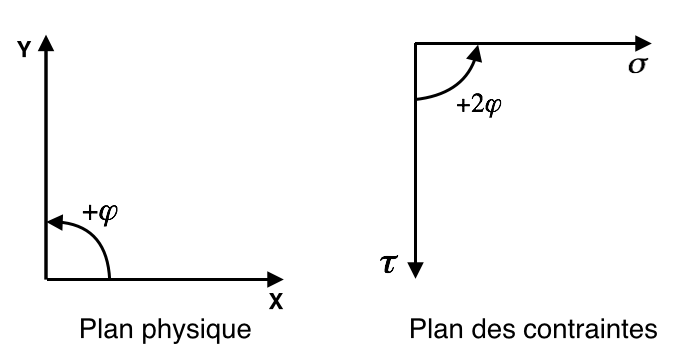
\includegraphics[scale=0.6]{tp2-1}
\end{center}

\textbf{Dans le plan physique, l'orientation de la facette est celle de $\sigma$ et $\tau$ est perpendiculaire, pointant vers la contrainte de plus grand module !}
\begin{center}
	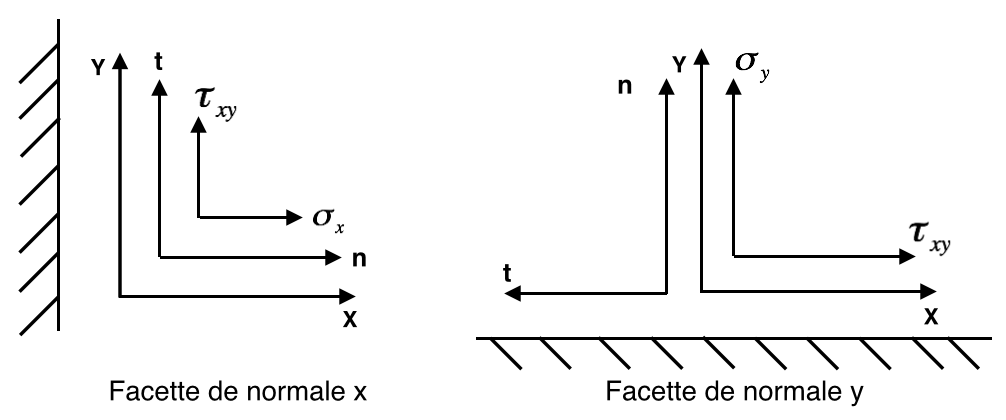
\includegraphics[scale=0.6]{tp2-2}
\end{center}

\subsection*{Construction}
\begin{equation}
	\overline{\overline{T}} = 
	\left(	
	\begin{array}{cc}
		\sigma _x  & \tau _{xy} \\ 
		\tau _{xy} & \sigma _y  
	\end{array}
	\right) \mbox{ est connu }
\end{equation}
Les composants de la matrice sont les composants du tenseur dans le cercle de Mohr. De cette manière, \textit{x} est représentatif de la facette de normale \textit{x} et \textit{y} pour la facette de normale \textit{y}. On a

\begin{equation}
	x(\sigma _x , \tau _{xy}) \qquad y(\sigma _y, - \tau _{xy})
\end{equation}

\begin{itemize}
	\item Valeurs principales : $\sigma _1$ et $\sigma _2$
	\item Directions principales : angle entre l'horizontale et x
	\item Valeurs extrémales : $\tau _{max}$ et $\tau _{min}$
\end{itemize}
	\section*{TP 3 : Maser à amoniac}
\begin{itemize}
	\item Equation de Schrödinger stationnaire à une dimension 
		\begin{equation}
			H\psi = E\psi \quad \Leftrightarrow \quad \left[\frac{-\hbar ^2}{2m}\frac{d^2}{dx^2} + V(x)\right]\psi = E \psi
		\end{equation}
		\item Pour un potentiel plus complexe de la forme 
			\begin{equation}
				\left\{ 
				\begin{aligned}
				&0 \qquad a< &|x| <b \\
				&V_0 \qquad &|x|<a \\
				&\infty \qquad &|x|>b
				\end{aligned}
				\right.
			\end{equation}
			La résolution de l'équation de Schrödinger devra être suivie de l'application des \textbf{conditions de continuité} et des \textbf{conditions aux limites} qui, dans ce cas, serait du type
				\begin{equation}
				\left\{ 
				\begin{aligned}
				\psi (x_0^+) &= \psi (x_0^-) \\
				\psi '(x_0^+) &= \psi '(x_0^-)
				\end{aligned}
				\right.
				\qquad
				\mbox{et}
				\qquad 
				\left\{ 
				\begin{aligned}
				\psi (b) &= 0 \\
				\psi (-b) &= 0
				\end{aligned}
				\right.
				\end{equation}
				Ils sont ainsi les \textbf{conditions de quantification de l'énergie}.
		
		\item Pour obtenir l'équation de Schrödinger non-stationnaire, il suffit de multiplier par l'exponentielle
			\begin{equation}
				-i\hbar \frac{d}{dt}\psi = H \psi \quad \Rightarrow \quad \phi _i(x,t) = \psi _i (x) \exp \left( \frac{-iE_i t}{\hbar}\right) 
			\end{equation}
\end{itemize}


	\section*{TP 4 - 5 : Hydrostatique}
\subsection*{Principe d'Archimède}
\begin{itemize}
	
	\item Soit $\overline{A}$ l'action du fluide sur le corps
	      \begin{equation}
	      	\overline{A} = \oint _S (-p) \overline{n} \, dS 
	      \end{equation}
	      	
	\item Equilibre du corps immergé : $\overline{A} + \overline{R} = 0$
	\item $\overline{R}$ : Résultante des forces exercées sur le corps sous l'action du fluide
	\item $\overline{A}$ : Résultante des forces de pression exercées par le fluide sur le corps
	\item \textbf{Postulat} : \textit{L'équilibre ne change pas si on remplace le corps immergé par du fluide}
	      \begin{equation}
	      	\int _V -\rho _f g \overline{1}_z \, dV + \overline{A} = 0 \quad \Rightarrow \quad \overline{A} = \int _V \rho _f g \overline{1}_z \, dV
	      \end{equation}
	\item \textbf{Attention} : il faut que tout le volume soit immergé pour appliquer Archimède
\end{itemize}

\subsection*{Principe de Pascal}

\begin{equation}
	p + \rho g z = cst
\end{equation}
\noindent Si en un point du fluide incompressible en équilibre isotherme, la pression est accrue de $\Delta p$, tous les points subissent cet accroissement

\subsection*{Répartition des pressions sur un obstacle}
\begin{itemize}
	\item La pression est toujours orienté selon la normale à la surface
	\item On choisit une pression de référence : $p_{ref} = 0$ ou $p_{ref} = p_{atm} = 101325 \, Pa$
	\item On trouve l'évolution de la pression grâce au principe de Pascal
\end{itemize}
\ \\
\begin{minipage}{0.55 \textwidth}
	\begin{flushleft}
		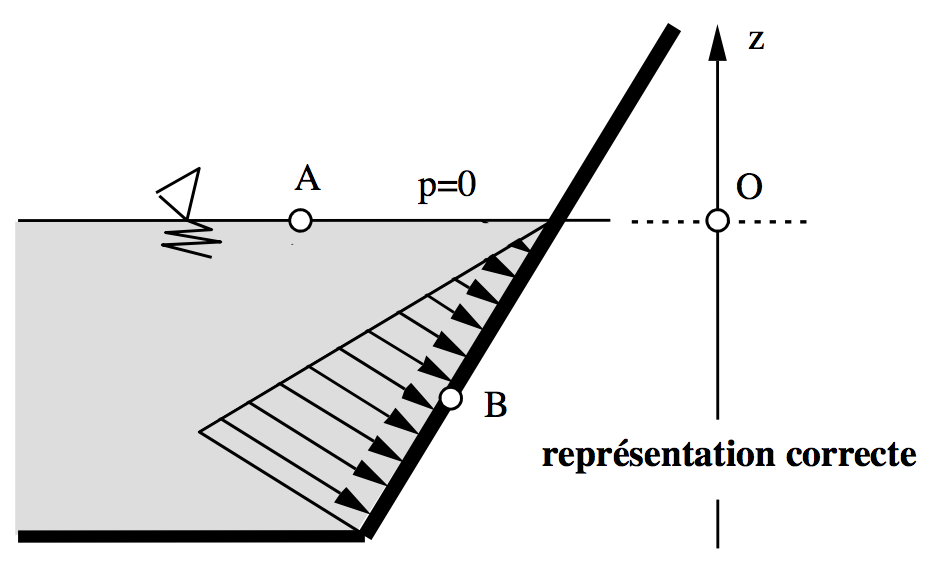
\includegraphics[scale=0.5]{tp4-1}
	\end{flushleft}
\end{minipage}
\begin{minipage}{0.5 \textwidth}
	\begin{flushleft}
		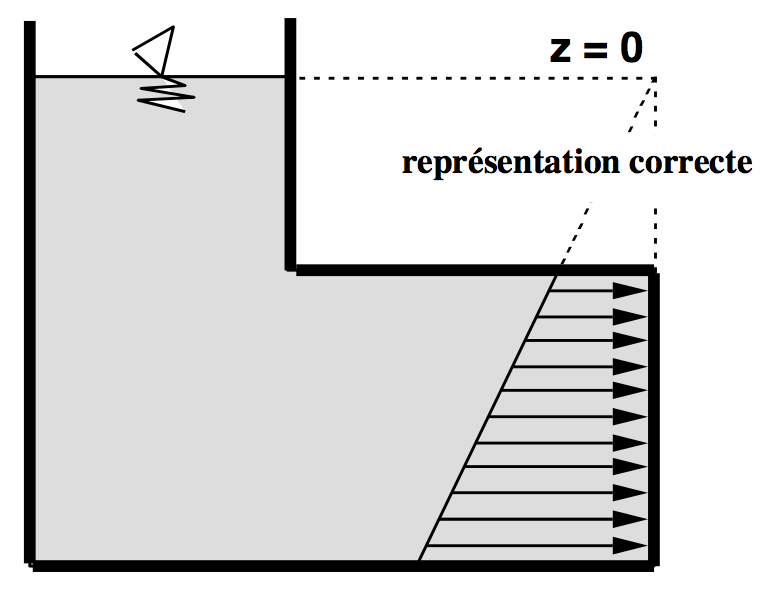
\includegraphics[scale=0.5]{tp4-2}
	\end{flushleft}
\end{minipage}
	
\section*{TP 5 : Moments cinétiques orbital et de spin, polarisation de la lumière}

\subsection*{Moement cinétique orbital}
\begin{itemize}
	\item On a $\vec{L} = (L_x,L_y,L_z)$ qui est obtenu par
		\begin{equation}
			\vec{L} = \vec{r} \times \vec{p}
		\end{equation}
		
	\item Commutation
		\begin{equation}
			[L_i,L_j] = i\hbar L_k \qquad et \qquad[L^2,L_i] = 0
		\end{equation}
	
	\item Fonctions propres communes à $L^2$ et $L_z$
		\begin{equation}
			Y^m_l (\theta , \phi ) = c_{norm} \cdot e^{im \varphi } \cdot \sin ^{|m|}(\theta ) \cdot p^{l-|m|}(\cos \theta )
		\end{equation}
		avec $l$ et $m$ respectivement le \textbf{nombre quantique de moment cinétique orbital} et \textbf{nombre quantique magnétique} (projeté sur l'axe z)
		
		\item Avec $l$ naturel et $m \in [-l,l] \Rightarrow (2l+1)$ valeurs de $m$
		\begin{equation}
			\left\{
			\begin{aligned}
			L^2 Y^m_l (\theta , \varphi ) &= \hbar ^2 l(l+1) Y^m_l (\theta , \varphi )\\
			L_z Y^m_l (\theta , \varphi ) &= \hbar m Y^m_l (\theta , \varphi )
			\end{aligned}
			\right.
		\end{equation}
\end{itemize}

\subsection*{Moment cinétique de spin}

\begin{itemize}
	\item On a $\vec{S} = (S_x,S_y,S_z)$ où les $S_j$ sont les \textbf{matrices de Pauli} 
		\begin{equation}
			S_i = \frac{\hbar}{2}\sigma _i
		\end{equation}
		avec
		\begin{equation}
			\sigma _x = 
			\left(
			\begin{array}{cc}
			0 & 1 \\ 
			1 & 0
			\end{array}
			\right)
			\qquad
			\sigma _y = 
			\left(
			\begin{array}{cc}
			0 & -i \\ 
			i & 0
			\end{array}
			\right)
			\qquad
			\sigma _x = 
			\left(
			\begin{array}{cc}
			1 & 0 \\ 
			0 & -1
			\end{array}
			\right) 
		\end{equation}
	
	\item Commutation
		\begin{equation}
			[S_i,S_j] = i\hbar S_k \qquad et \qquad[S^2,S_i] = 0
		\end{equation}
		
	\item Fonctions propres communes à $S^2$ et $S_z$
		\begin{equation}
			\chi ^{m_s}_s \qquad (spineur)
		\end{equation}
	où $s$ est le \textbf{spin} et $m_s$ la projection du spin sur l'axe z. 
	
	\item pour l'électron, le protion et le neutron, le spin vaut $1/2$ et on les appelle \textbf{fermion}
	
	\item Avec $s = 1/2$ et $m_s \in [-s,s] \Rightarrow m_s = \pm 1/2 \Rightarrow(2s + 1)$ valeurs
		\begin{equation}
			\left\{
			\begin{aligned}
			S^2 \chi _{m_s} &= \hbar ^2 s(s+1) \chi _{m_s} = \frac{3}{4}\hbar ^2 \chi _{m_s}\\
			S_z \chi _{m_s} &= \hbar m_s \chi _{m_s} = \pm \frac{1}{2}\hbar \chi _{m_s} 
			\end{aligned}
			\right.
		\end{equation}
		
	\item Photon $\Rightarrow s = 1$ et on les appelle \textbf{Boson}
	
	\item Etat \textbf{up} (à gauche) et état \textbf{down} (à droite)
		\begin{equation}
			\chi _{\frac{1}{2}} = 
			\left(
			\begin{array}{c}
			1 \\ 
			0
			\end{array}
			\right) 
			\qquad
			\chi _{-\frac{1}{2}} =
			\left(						
			\begin{array}{c}
			0 \\ 
			1
			\end{array} 
			\right)		
		\end{equation}
		
\end{itemize}
	
\section*{TP6 : Système hydrogénoïde}

\begin{itemize}
	\item Unité : le Rydeberg
		\begin{equation}
			a_0 = \frac{4\pi \epsilon _0 \hbar ^2}{m_e e^2} = 0,529 .10^{-7} \, mm \qquad Ryd = \frac{\hbar ^2}{2m_e a_0^2} = \frac{e^2}{8 \pi \epsilon_0 a_0} = 13,6 \, eV
		\end{equation}
		
	\item Fonction d'onde 
		\begin{equation}
			\psi _{Hyd} (\vec{R}) = R_{nl} (r) Y^m_l (\theta , \varphi )
		\end{equation}
		où, pour l'état 1s de l'hydrogène seulement (les autres sont donnés par une formule dégueu qui sera sans doute donnée)
		\begin{equation}
			R_{nl} = 2\left( \frac{Z}{a_0} \right) ^{3/2} e^{-\frac{Zr}{a_0}}
		\end{equation}
		
	\item Intégrale de normalisation \\
	Lorsqu'on nous demande de vérifier si les fonctions $R_{nl}$ et $Y^m_l$ sont normées, il faut intégrer respectivement selon 
	\begin{equation}
	r^2 dr \qquad et \qquad \sin \theta \, d\theta \, d\varphi
	\end{equation}
	\item Energie quantifié 
		\begin{equation}
			E_n = -\frac{Z^2}{n^2}Ryd
		\end{equation}
		avec 
			\begin{itemize}
				\item $n = n_R +l +1 \geq 1$
				\item $l \in \mathbb{N} = 0,1,2, \dots \Rightarrow$ couches s, p, d, f, g, $\dots$		
				\item $m \in [-l,l]$
			\end{itemize} 
	
	\item Système hydrogénoïde
		\begin{equation}
			a_0, Ryd \qquad \Leftrightarrow \qquad a_\mu = \frac{m_e}{\mu } a_0, Ryd_\mu = \frac{\mu }{m_e} Ryd
		\end{equation}
		avec $\frac{1}{\mu} = \frac{1}{m_1}+\frac{1}{m_2}+ \dots$
\end{itemize}
	
\section*{TP 7 : Composition de moments cinétiques}
\begin{itemize}
	\item $\vec{L} = \vec{r}\times \vec{p} = -i\hbar (\vec{r}\times \vec{\nabla})$
	
	\item $\vec{S} = spin$ et $s$ est le nombre quantique de spin qui soit 
	\begin{equation}
		s \in \frac{\mathbb{N}}{2} = \left\{ \frac{1}{2}, \frac{3}{2},\dots \right\} \, (fermions) \qquad soit \qquad s \in \mathbb{N} \, (bosons)
	\end{equation}
	\item $m_s$ : projection du spin sur l'axe z et varie par pas de 1 entre $-s \leq m_s \leq s$
	
	\item $l$ : nombre quantique de moment cinétique orbital ($l \in \mathbb{N}$)
	
	\item $m$ : nombre quantique magnétique avec $m \in \mathbb{Z} \ |\, -l \leq m \leq l$
	
	\item Pour un nombre qjuantique quelconque $\underbrace{\vec{j}}_{j,m} = \underbrace{\vec{j_1}}_{j_1,m_1}+\underbrace{\vec{j_2}}_{j_2,m_2}$ alors on utiilse la \textbf{relation triangulaire} 
	\begin{equation}
	|j_1 -j_2| \leq j \leq j_1+j_2
	\end{equation}
	
	\item Le nombre de valeur possible pour $m$ est toujours $2 j +1$ valeurs
	
	\item Dans le cas d'un électron plongé dans un champ magnétique, il faut tenir compte de l'action de ce champ dans le hamiltonien en rajoutant un terme $W$ au hamiltonien de l'état non perturbé $H_0$
	\begin{equation}
		H = H_0 + W
	\end{equation}
	avec $W = -\vec{M}\vec{B}$ et $\vec{M} = -\frac{e}{2m_e}(\vec{L}+g.\vec{S})$. g est le facteur gyromagnétique $\approx 2$
\end{itemize}
	
\section*{TP 8 : Les atomes}
\begin{itemize}
	\item Moment cinétique $\vec{J}$ (opérateur vectoriel) : 2 nombre quantiques
		\begin{itemize}
			\item $j$ ($\geq 0$) : entier ou demi-entier (valeur propre de $J^2 = \hbar ^2 j(j+1)$)
			\item $m \in [-j,j]$ pour un total de $2j +1$ valeurs entières ou demi-entières (valeur propre de $J_z = \hbar m$)
		\end{itemize}
		
	\item Composition de moment cinétique
	\begin{equation}
		\vec{J} = \vec{J_1}+\vec{J_2} \Rightarrow |j_1-j_2| \leq j \leq |j_1+j_2|
	\end{equation}
	\begin{itemize}
		\item Structure fine : $\vec{J}=\vec{L}+\vec{S}$
		\item Structure hyperfine : $\vec{F} = \vec{J}+\vec{L}$ (spin du noyau)
	\end{itemize}
	
	\item Système hydrogénoïde : état = $(n,l,m,m_s \, (= \pm 1/2)$ avec $n_r = n+l+1$
	\begin{itemize}
		\item $l$ donné : $(2l+1)$ valeurs de $m$ et 2 valeurs de $m_s \Rightarrow 2.(2l+1)$ états
		
		\item $l = 0,1,2, \dots \Rightarrow s,p,d,f,g,\dots$
		
		\item Sous-couche ($nl$) fermée : $l = 0 \Rightarrow J(atome) = J(dernière$ $couche)$
		
		\item Notation spectroscopique (dernière couche atome)
		\begin{equation}
			^{2S+1}L_J
		\end{equation}
		\begin{itemize}
			\item $L$ et $S$ : moment cinétique orbital et spin \textbf{total} de la dernière couche
			
			\item Helium : toujours un électron en $1s$ (stabilité)
		\end{itemize}
	\end{itemize}
\end{itemize}
	
\section*{TP 9 : Rotation et vibration des molécules diatomiques}
\begin{itemize}
	
	\item Vibration de molécules diatomiques
		\begin{itemize}
			
			\item Approximation parabolique 
				\begin{equation}
				V = \frac{1}{2}\mu \omega ^2 (R-R_0)^2
				\end{equation}
					
			\item Energie de vibration valable à courtes distances 
				\begin{equation}
				E_{n,vib} = (n+\frac{1}{2})\hbar \omega
				\end{equation}
			\end{itemize}
		
		\item Rotation de molécules diatomiques
			
			\begin{itemize}
				\item Hamiltonien de rotation
					\begin{equation}
					H_{rot} = \frac{L^2}{2I} \qquad \Rightarrow \qquad E_{l,rot} = \frac{\hbar ^2 l(l+1)}{2I} \qquad avec \ I = \mu r_0 ^2
					\end{equation}
				
				\item Classification des différentes énergies
					\begin{equation}
					E_{rot} < E_{vib} < Ryd
					\end{equation}
			\end{itemize}
			
		\item Transition dipolaire électrique $\Delta l = 1$

			\begin{itemize}
				\item Absorption : $l_f = l_i + 1$
				\item Emission : $l_f = l_i - 1$
				\item Les raies d'absorption et d'émission correspondent aux énergies de transition admises
			\end{itemize}
\end{itemize}

\begin{figure}[h]
	\begin{center}
		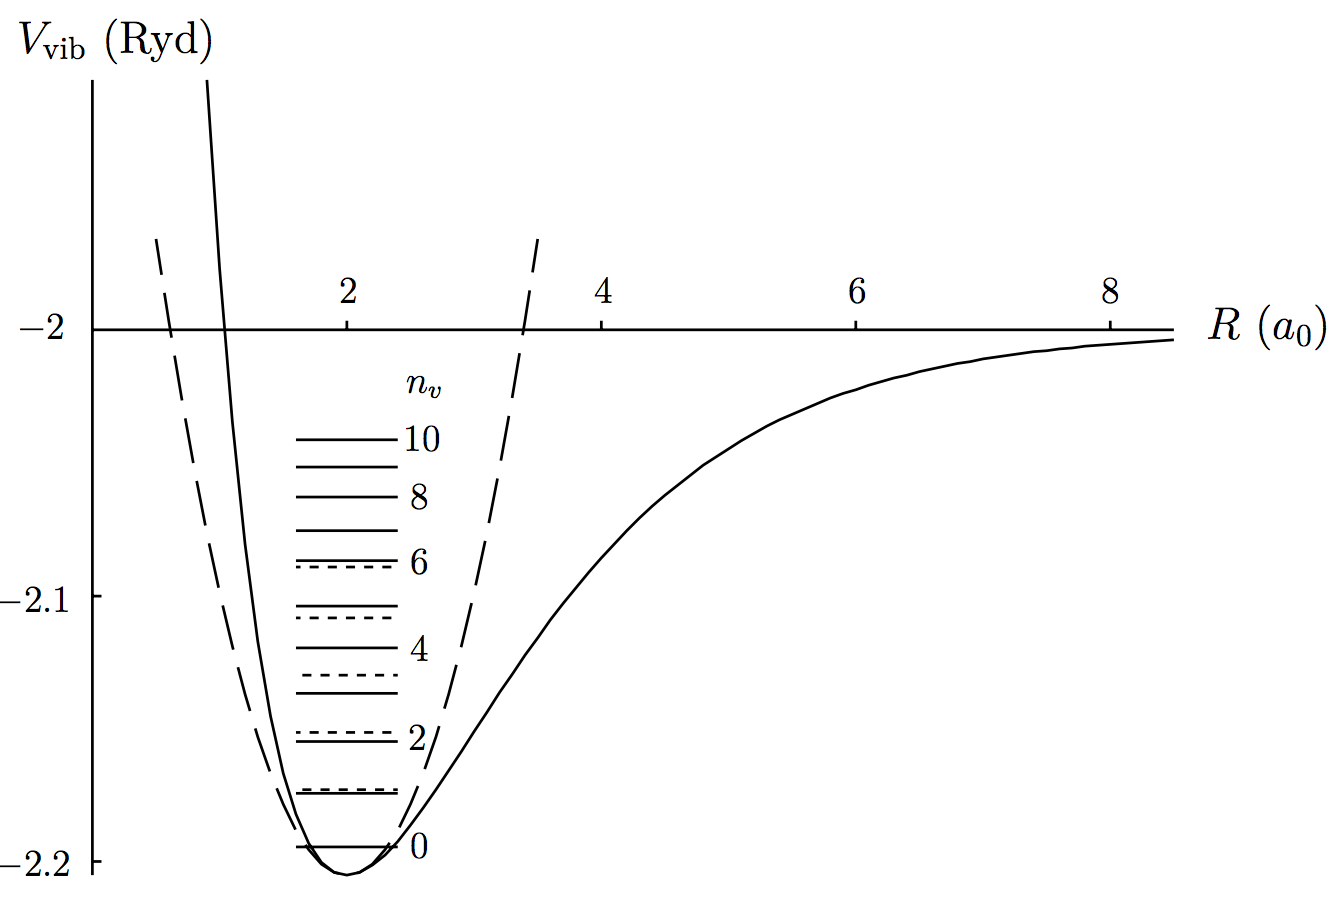
\includegraphics[scale=0.5]{img/1}
		\caption{Spectre de vibration de la molécule $H_2$.}
	\end{center}
\end{figure}
	%\chapter{Annexe 1}
Coucou
	
	
\end{document}